\chapter{Transformer}
\label{chap:transformer}

先从一次具体的阅读理解说起。读懂“猫追狗”，关键不是逐个认出三个字，而是把它们之间的关系连起来：更新“追”的表示时，既要看清它前面的“猫”是谁在追，也要看清它后面的“狗”在追谁；前后两个位置的信息缺一不可。若任务换成续写“猫追”，同样需要读取别处的信息，但允许读取的范围不同——“狗”这个字此刻还没有产生，只能依据已经给定的“猫追”两个字去预测。第\ref{sec:rnn-attention}节的循环注意力已经让解码器按当前需求读取源表示，但无论源表示还是解码状态，都仍要沿时间一步一步递推形成。面对这两个任务，自然会产生两个新的问题：对于已经完整给定的输入，能不能不再串行等待，让各个位置在同一层里直接交换信息？对于尚未产生的输出，又怎样保证每次读取只用到预测当时真正已知的内容？

Transformer正是对这两个问题的回答。它用注意力选择读取的来源，让每个位置按需直接访问其他位置的表示；用层间堆叠把读取结果反复组合，从而逐层建立更复杂的关系。顺序不再由递推隐含地携带，而是通过位置表示和连接约束显式地进入计算；监督目标则决定哪些输出接受误差反馈。与此同时，保存多少个位置的表示、在多少对位置之间建立连接，直接决定了所需的计算量和存储量——这也是理解本章众多扩展方法的一条主线。本章先建立Transformer的网络结构和梯度计算，再比较位置编码、注意力、前馈层与连接方式的各类扩展，分析有关学习的结论各需什么条件，最后把这些构件接到分类、转换、生成和图像任务上。

\FloatBarrier
\section{Transformer概述}
\label{sec:transformer-overview}

一段输入完整给定后，为什么还要保留循环式的逐时间步处理？既然每个词元都已经摆在眼前，更直接的做法是：让各位置先各自形成一个表示，然后在同一层里同时读取彼此，得到新的表示，下一层再基于这些新表示继续读取。Transformer正是按这种方式组织位置交互的。注意力的发展回答了“怎样选择要读取的信息”，架构的发展则回答了“如何把这套读取接到不同的预测任务上”。需要提前说明的是，这种并行不是免费的：每个位置都要和其他位置逐一比较，于是计算量随序列长度平方增长，逐位置表示也都要保存下来。理解便利与代价并存，是理解Transformer及其众多效率扩展的前提。

\subsection{从循环计算到位置间读取}
\label{sec:transformer-core-idea}

循环注意力中的查询来自解码状态，候选表示来自编码状态；它使每一步可以重新选择上下文，却保留了状态递推。\term{自注意力}（self-attention）把查询和候选表示都取自同一组输入：每个位置根据自身表示，选择同一序列中其他位置的信息。例如，在“这部电影并不精彩”中，表示“精彩”的位置可以直接读取“并不”，形成带有上下文的表示。否定上下文能否进入最终判断，取决于学到的权重、被读取的值及后续变换；直连使这条信息路径在结构上可用。

\term{Transformer}是一类以注意力进行位置间交互、以逐位置前馈网络进行特征变换的网络。一次读取使用该层入口已有的表示，因而同层各位置可以同时更新；下一层再读取这些新表示。稠密自注意力为允许读取的位置对建立直接路径。来自多个位置的信息汇入加权混合，任务所需的差别还要由值特征和后续变换保留。

用“信息要走多远”可以看清这次改变的分量。在循环网络中，第1个位置的信息要到达第$n$个位置，必须依次穿过$n-1$个时间步的状态更新，每一步都可能被压缩或稀释；自注意力则在它们之间直接连一条边，无论相隔多远，一层之内就能读到。直连缩短了信息和梯度的传播路径，代价是连接数从与长度同阶增长到与长度平方同阶，并且要为每个位置保存可供读取的表示。读取范围还可以按需裁剪：理解任务允许每个位置读取整段，生成任务则用掩码把每个位置限制在它当时的已知前缀上。这样，同一套读取机制既能服务并行的整段理解，也能服务严格按次序进行的生成。

\subsection{注意力机制的发展}
\label{sec:transformer-attention-history}

注意力机制始终围绕一个问题展开：当前计算应该优先使用哪些信息？早期视觉模型通过选择观察位置分配处理资源，后来的序列模型通过可学习权重读取已有表示。沿着这两条相互交汇的路线，可以看清注意力如何从局部选择机制发展为Transformer中的基本运算。

\paragraph{早期视觉注意力：选择在哪里观察}
1985年，Koch与Ullman提出选择性视觉注意力的计算模型：不同视觉特征共同形成\term{显著图}（saliency map），即标出各位置有多突出的空间分布；模型选出突出位置，再抑制已选位置，使注意转向其他区域。这类模型解释观察资源的空间分配；后文的查询、键和值则描述已有表示之间的加权读取\scite{koch1985attention}

神经网络随后被用于学习观察策略。Schmidhuber与Huber在1991年的工作中，用神经控制器移动“人工中央凹”，即中心精细、外围粗略的局部观察区域，以逐步找到和跟踪目标。控制器借助学到的环境模型改进移动轨迹，观察位置由这一策略产生\scite{schmidhuber1991attention} 2014年，Mnih等用循环网络整合多次局部观察，并学习下一次观察的位置。这种先采样位置、再读取局部输入的方式属于\term{硬注意力}（hard attention）；论文从高斯策略中采样连续位置坐标。局部读取操作无法沿常规可微路径直接优化，观察策略因而用策略梯度训练\scite{mnih2014attention}

\paragraph{机器翻译：从固定上下文到软对齐}
序列转换遇到的是另一种信息瓶颈：编码器已经读完整句，但若只把一个固定向量交给解码器，每个目标词都要从同一压缩结果中恢复细节。Bahdanau、Cho与Bengio于2014年发布、2015年发表于ICLR的工作保留所有源位置的编码状态，在生成每个目标词之前，用此前的解码状态重新为这些源状态评分。得分经Softmax变成权重，再加权求和，形成随生成步变化的上下文。多个源位置共同提供信息，权重随翻译目标学习，聚合运算可微；这就是\term{软注意力}（soft attention）形成的软对齐\scite{bahdanau2015}

例如翻译“猫追狗”时，预测cat与预测dog所需的源信息不同，读取权重可以随之改变；“对齐”表示目标步与源位置之间学到的软对应，其监督来自翻译目标。这项工作中的加性注意力用一个小前馈网络评估两种状态是否匹配，具体公式已见式\eqref{eq:rnn-additive-attention}。每次读取随目标步改变，源表示的形成和目标状态的更新则继续使用循环递推。

2015年，Luong等系统比较了直接点积、带参数的双线性形式等评分方式，并区分读取全部源位置的全局注意力与只读取一个窗口的局部注意力。这使“怎样评分”和“允许读取哪些位置”成为可分别选择的设计；局部方案规定候选窗口，窗口内部仍可对多个位置软加权\scite{luong2015} 同年，Xu等的Show, Attend and Tell将基于内容的注意力用于图像描述：生成不同词时，语言解码器可以对不同图像区域分配权重，论文同时研究了软聚合与随机硬选择。被读取对象由源词变为图像区域，按当前需求选择信息的作用保持不变\scite{xu2015showattend}

\paragraph{自注意力：从读取另一序列到建立内部关系}
注意力还可以用来联系同一序列中的位置。2016年，Cheng等在用于机器阅读的LSTM记忆网络中保存此前词元的表示，并让当前词元通过注意力读取这些记忆，建立序列内部关系。这种\term{序列内注意力}（intra-attention）是自注意力的一种早期实现，网络仍保留循环更新；这项设计改变了读取来源，循环更新继续安排表示形成的次序\scite{cheng2016reading}

上述模型改变了不同环节：硬选择和软聚合规定怎样取出信息，加性和点积规定怎样评分，交叉与自注意力规定表示来自哪组位置。评分方式、信息来源和读取范围可以组合；第\ref{sec:transformer-attention}节将用查询、键和值统一描述这些角色，再展开Transformer采用的计算形式。

\subsection{Transformer的提出与演进}
\label{sec:transformer-architecture-history}

注意力机制使解码器可以反复读取源表示，但这些表示最初仍由循环网络产生。1997年的LSTM通过记忆单元与控制门改善长距离信息的保留和梯度传递，更新仍沿时间进行\scite{hochreiter1997} 2014年，Sutskever等用LSTM编码器—解码器进行序列转换，将输入压缩到固定维表示\scite{sutskever2014seq2seq} 第\ref{sec:transformer-attention-history}节介绍的软对齐进一步减轻了固定表示的瓶颈，循环递推却仍限制整段输入表示的并行形成。

2017年，Vaswani等在机器翻译中提出Transformer：源端以自注意力形成上下文，目标端以因果自注意力形成前缀表示，再用交叉注意力读取源端。位置表示提供顺序，多头读取形成多组聚合，逐位置前馈层变换特征。这一设计把位置间的循环更新改为注意力读取与层间堆叠，为已知序列提供批量矩阵计算方式\scite{vaswani2017}

形成表示的读取规则也开始服务于不同预训练目标。2018年，GPT用因果Transformer进行语言模型预训练，再适配有监督任务\scite{radford2018gpt} 同年发布、2019年发表于NAACL的BERT用双向编码器从被遮蔽的输入恢复词元，形成可用于多种理解任务的表示\scite{devlin2019} 2020年发表的T5研究把任务统一为文本输入到文本输出，采用编码器—解码器组织条件生成\scite{raffel2020t5} 第\ref{sec:transformer-common-architectures}节将比较这些架构；预训练数据和迁移范式由相关章节展开。

\subsection{与RNN/LSTM的比较}
\label{sec:transformer-recurrent-comparison}

与RNN/LSTM相比，关键变化在于历史信息的组织方式。普通循环网络把过去压缩进固定宽度状态；LSTM增加记忆与门，改善保留方式，但仍需经中间时间步传递。稠密自注意力保存各位置的表示，让当前位置直接读取所需历史。远处证据因此可沿一层连接到达，同时更多位置的键和值需要留存。配有注意力的循环模型还可以保存源位置表示，其历史存储和读取应把这一额外部分计入。表~\ref{tab:transformer-rnn-comparison}固定长度和宽度，比较三种基础结构。

并行计算的条件是所需输入已经给定。训练自回归模型时，真实目标序列已知，可以一次送入移位后的目标，并用掩码限制各位置读取；生成时，下一个词元尚未确定，仍需根据已有前缀产生它，再继续下一步。已知序列的各位置表示可以并行形成；自回归输出则按新词元到达的次序逐步延长。

全局读取也有成本。设序列长为$n$，表示宽度为$d$，常规多头注意力的各头总宽度与$d$同阶，一层自注意力的位置对计算需要$O(n^2d)$次算术操作，投影另需$O(nd^2)$。直接保存各头权重需要$O(hn^2)$个元素，其中$h$为头数。与固定宽度的循环状态相比，Transformer保存和读取了更多逐位置信息；后文将区分减少连接、改变聚合公式和改善存储方式三种路线。适用场景包括文本、连续时间观测和图像块等可表示为向量序列的输入，这些任务的顺序、局部关系和可见范围由位置表示、连接及输入协议继续规定。

\begin{table*}[htbp]
  \centering
  \small
  \begin{tabular}{@{}p{28mm}p{39mm}p{40mm}p{48mm}@{}}
    \toprule
    比较维度 & 基础RNN & LSTM & 稠密Transformer自注意力 \\
    \midrule
    历史表示 & 固定宽度隐藏状态 & 隐藏状态与记忆单元 & 每层保留逐位置键和值 \\
    顺序来源 & 时间递推 & 时间递推及门控 & 位置表示与可见性约束 \\
    已知整段的计算 & 同层沿时间串行 & 同层沿时间串行 & 同层位置可并行，层间依赖仍在 \\
    远位置的结构路径 & 经中间时间步，$O(n)$ & 经中间时间步，$O(n)$ & 允许直连时，一层内$O(1)$ \\
    单层整段算术量 & $O(nd^2)$ & $O(nd^2)$，门增加常数 & $O(n^2d+nd^2)$ \\
    生成时的历史存储 & $O(d)$ & $O(d)$ & 常规KV缓存为$O(nd)$ \\
    \bottomrule
  \end{tabular}
  \caption{固定输入及隐藏宽度同阶为$d$、序列长为$n$的结构比较。历史存储按单层、单样本统计，省略训练激活和参数；Transformer各头总宽度与$d$同阶。最短连接路径不保证实际依赖一定学会，算术量也不直接等于运行时间。三者在标准自回归生成时都逐步产生输出。}
  \label{tab:transformer-rnn-comparison}
\end{table*}

\FloatBarrier
\section{网络结构}
\label{sec:transformer-structure}

下面沿输入表示、位置读取、逐位置变换与任务输出说明计算。以长度为$n$的一段输入建立共同记号。隐藏表示宽度为$d$，网络块数为$L$，第$l$个块后的矩阵为$\bm H^{(l)}\in\mathbb R^{n\times d}$，按行存放各位置的列向量，即$\bm H_{i,:}^{(l)}=(\bm h_i^{(l)})^{\top}$。括号上标表示层间更新编号，位置使用下标。这里讨论单个样本；批量计算另加样本维，并分别处理有效长度。

在进入公式之前，先给出一个块内各构件分工的整体印象，读者可以带着这条线索阅读后面的小节。原始输入先要经过查表或投影变成统一宽度的向量，并补上位置信息；随后每个Transformer块重复四件事：注意力让各位置之间交换信息（负责“从哪里读”），前馈网络对每个位置读到的结果各自做一次非线性特征加工（负责“读到之后怎么消化”），残差连接把加工前的旧表示原样保留并加回（负责“在已有基础上学增量，而不是推倒重来”），层归一化则把每个位置一行特征的尺度校准（负责“让层层叠加时数值不失控”）。多个这样的块堆叠起来，最后按任务接上不同的输出头：整段分类、逐位置标注，还是逐词生成。位置交互与逐位置加工交替进行，是这套结构最核心的节奏。

\subsection{输入表示与位置编码}
\label{sec:transformer-input}

注意力接收向量，原始输入需要先转为统一宽度。文本中的\term{词元}（token）是分词系统采用的离散单位，可以是词、子词或符号。设词表大小为$v$，位置$i$的词元编号为$u_i$，嵌入矩阵为$\bm E\in\mathbb R^{v\times d}$，则$\bm e_i=(\bm E_{u_i,:})^{\top}$。同一词元的各次出现从同一行参数取出内容向量；之后的网络将它与位置和上下文组合，产生各次出现自己的隐藏表示。

若输入是$\bm x_i\in\mathbb R^p$的连续观测，可以用$\bm e_i=\bm W_{\mathrm{in}}\bm x_i+\bm b_{\mathrm{in}}$投影到$d$维，其中$\bm W_{\mathrm{in}}\in\mathbb R^{d\times p}$。图像可以先分为小块，再把每块的像素或前端特征展平并投影。三种接口都产生注意力可读取的向量。文本顺序、实际时间间隔、图像坐标及观测缺失可以加入这些向量或相应读取规则，使任务所需关系也进入模型。

在“猫追狗”和“狗追猫”中，词元相同，动词两侧的角色却交换了。网络需要从输入中获得这个顺序差别。递推式$\bm h_i=f(\bm h_{i-1},\bm x_i)$已经使第$i$步接收到“处理过前$i-1$项”的状态，交换输入会改变后续计算。自注意力的共享投影只看到内容向量与内容匹配，矩阵的第几行并不会自动变成网络可用的特征。仅使用词元嵌入时，同一个词元面对相同的内容集合；将位于动词之前或之后的信息加入计算后，模型才有区分施事与受事的输入依据。同一词元多次出现时，位置关系还帮助网络区分每次出现的作用。

这一缺口可以用计算性质精确表达。暂将一次自注意力记为$\operatorname{SA}(\bm H)$：每行输入分别经过三组共享的线性投影，得到发起读取的查询、用于匹配的键和供读取的值；查询与键的匹配得分组成矩阵$\bm S$，其中$S_{i,j}$表示位置$i$读取位置$j$的得分。每行得分经Softmax变成权重，再用这些权重聚合值。下一节会给出三组投影和点积评分的具体公式，这里先考察重排输入会怎样影响这条计算路径。

在不含位置表示和顺序掩码的情形中，对输入行施加置换矩阵$\bm P$。由于各行使用同一组投影参数，查询、键、值也同步重排，得分矩阵变为$\bm P\bm S\bm P^{\top}$：左乘重排查询行，右乘重排候选键列。逐行Softmax随之重排，因此
\begin{equation}
  \operatorname{SA}(\bm P\bm H)
  =\bm P\operatorname{SA}(\bm H)\text{。}
  \label{eq:transformer-permutation}
\end{equation}
共享的逐位置前馈层和归一化保留这一等变性。若再做平均读出，整段输出便对重排不变；“猫追狗”和“狗追猫”可能因只有相同内容向量而无法区分。因果掩码使位置只能读取此前输入，改变了上述置换条件。它规定连接范围；位置距离则还需要编码或由具体网络计算获得。某些因果模型可以借助边界和层间计算学习部分顺序，任务需要哪些关系仍由输入和结构决定。若输入本来是无序集合，保留置换等变性可以避免把保存编号引入预测。

\term{位置编码}（positional encoding）把元素所在位置或位置之间的关系加入表示计算。最直接的做法为每个位置设置$\bm p_i\in\mathbb R^d$，并令
\begin{equation}
  \bm h_i^{(0)}=\bm e_i+\bm p_i\text{。}
  \label{eq:transformer-input-position}
\end{equation}
这称为\term{绝对位置编码}（absolute positional encoding）：位置$i$本身有一个表示。可学习位置表与词元嵌入共同训练，正弦位置编码则按固定函数产生。相加要求维度一致；原始Transformer对词元嵌入乘以$\sqrt d$，以调整内容与位置的相对尺度，其他输入接口则可按自身尺度配置。

把这一步落到实际序列上，取“猫／追／猫”，暂把每个汉字当作一个词元；实际模型也可能采用子词等其他切分。两个“猫”查询同一行嵌入参数，因此位置1和3的内容向量相同。为便于手算，令嵌入宽度为4，猫的嵌入为$(0.20,-0.10,0.40,0.30)^{\top}$，追的嵌入为$(0,0.50,-0.20,0.10)^{\top}$。下列数值为便于复算而构造的教学嵌入。图中的词元矩阵$\bm E_{\mathrm{seq}}$与位置矩阵$\bm P_{\mathrm{pos}}$均按序列位置排列，形状为$3\times4$，以区别于完整词表参数表和置换矩阵。

图~\ref{fig:transformer-position-example}把内容与位置分成两条计算路径。假设词表给“猫”和“追”分配的编号分别是7和12，左图用词元编号$7,12,7$查嵌入表；中图从序列的先后顺序得到位置序号$1,2,3$，并代入四维正弦位置向量$\bm p_i=(\sin i,\cos i,\sin(0.01i),\cos(0.01i))^{\top}$，角度以弧度计。位置序号与词表编号不同，两个“猫”虽然查到同一个内容向量，仍会得到不同的位置向量。右图将两路表示按对应坐标相加，输出形状保持为$3\times4$。逐坐标相加保持四维宽度；沿特征维拼接则得到八维，需要相应修改后续接口。第\ref{sec:transformer-position-extensions}节会解释这些频率如何推广到任意偶数宽度，以及如何改为表示相对距离。

\begin{figure*}[htbp]
  \centering
  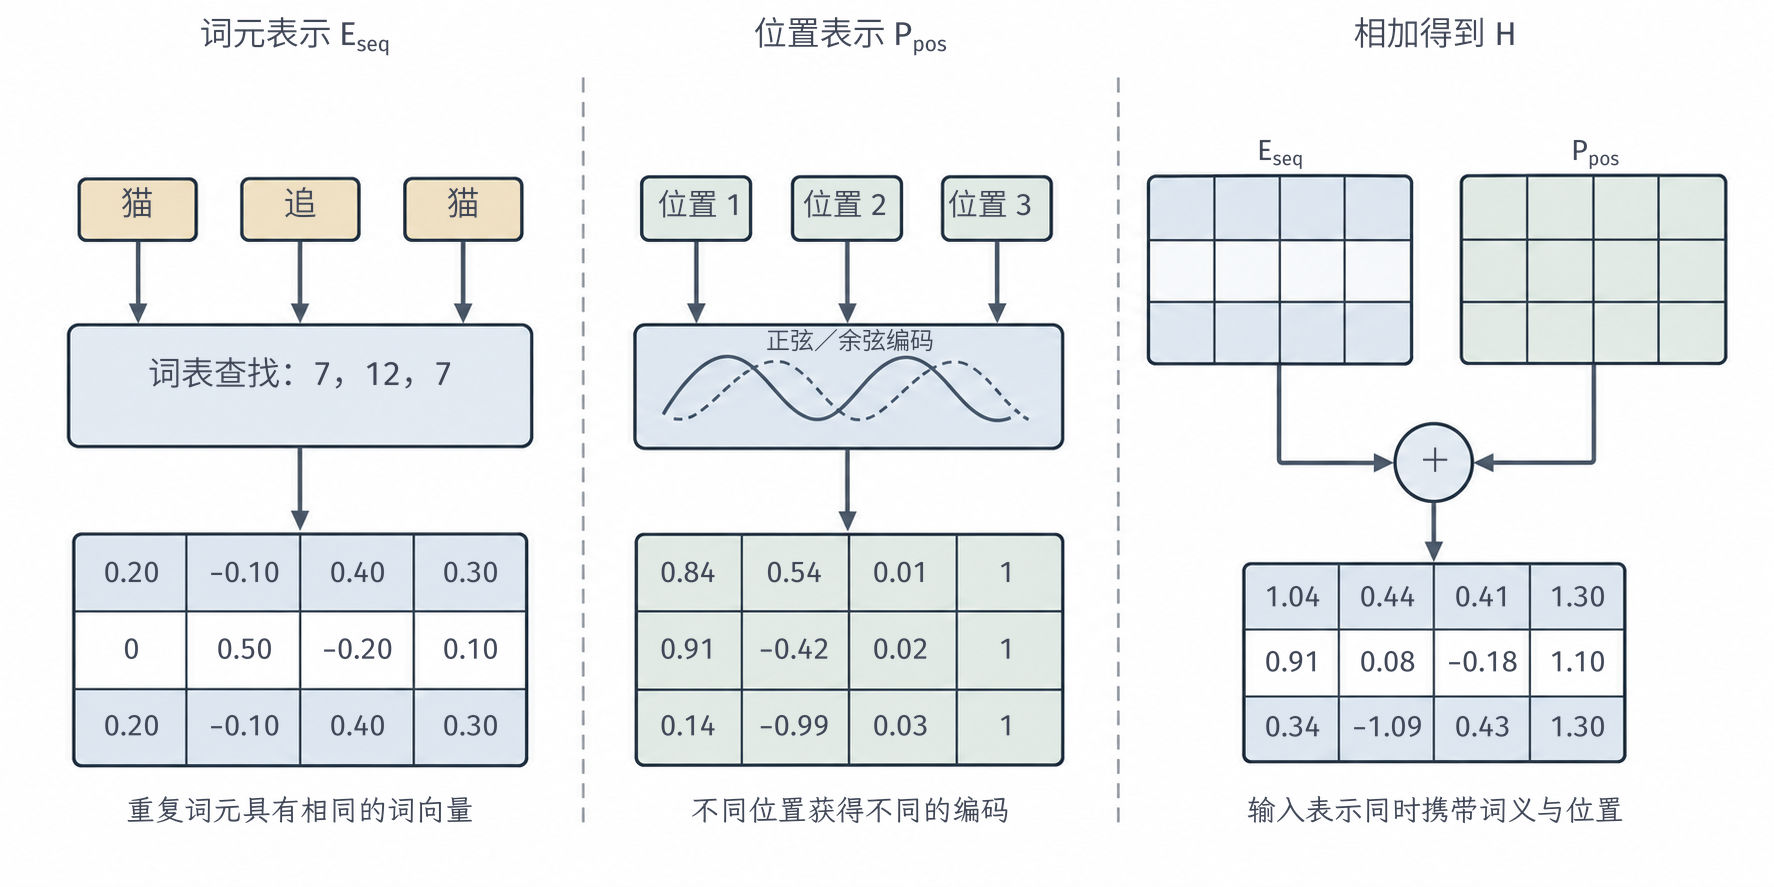
\includegraphics[width=150.199mm]{figures/05-neural-network-models/00-shared/generated/transformer-position-example/figure.png}
  \caption{序列“猫／追／猫”的输入构造。左图用词元编号查嵌入表，中图把位置序号代入正弦、余弦函数，右图将两组$3\times4$表示逐元素相加。三个矩阵的行均按输入位置排列，每格是一个特征值。两个“猫”共享内容向量，位置向量及最终表示却不同。词元编号和嵌入为教学设定；位置向量按弧度计算，数值保留两位小数，位置矩阵的最后一列显示相同是舍入所致。}
  \label{fig:transformer-position-example}
\end{figure*}

位置差异需要以能够留在后续表示中的方式编码。仅把编号$i$填在各坐标上，会遇到均值消除问题。例如，后文第\ref{sec:transformer-residual-normalization}节介绍的层归一化会减去一行的均值；若输入只加$i\bm1$并立即按行归一化，这个位置常数就会被消去。不同频率或可学习坐标提供了更丰富的位置差异。内容与位置进入同一表示后，训练才能据任务目标调整它们的组合与读取。

不等长序列可以填充到共同形状，真实位置由有效集合或长度记录。注意力排除填充键，池化只汇总真实位置，损失只统计有效监督位置。若将多段独立文本装入同一矩阵，也需限制跨段读取，并明确位置编号的重置方式；矩阵中相邻不等于任务中连续。

\subsection{注意力层}
\label{sec:transformer-attention}

第\ref{sec:transformer-attention-history}节已经介绍了注意力怎样根据当前需求读取信息。可以先把一次读取类比为查字典：手中待查的词是\term{查询}（query, Q），字典里用于匹配条目的词头是\term{键}（key, K），找到条目后读取的释义是\term{值}（value, V）。查询提出当前需求，键提供匹配特征，值提供被取出的内容；注意力中的键因此是表示向量，数组下标只负责存放它。

注意力把这种查询推广为连续的软匹配。输入经可学习投影得到查询、键和值，查询与键的连续得分再变成权重；多个值依权重共同形成输出。投影参数随训练调整，匹配方式也随之改变。这里把输入固定为“猫／追／狗”：更新“追”的表示时，网络需要结合谁在追、追的是谁；更新“猫”时，所需的上下文组合又可能不同。同一个位置在读取别人和被别人读取时承担不同作用，查询与键用于评分，值用于输出，三者不需要具有相同含义。

设查询输入为$\bm H_{\mathrm q}\in\mathbb R^{n_q\times d}$，被读取输入为$\bm H_{\mathrm s}\in\mathbb R^{n_s\times d}$。暂省略偏置，单头投影为
\begin{equation}
  \begin{aligned}
    \bm Q&=\bm H_{\mathrm q}\bm W_{\mathrm q},\qquad
    \bm K=\bm H_{\mathrm s}\bm W_{\mathrm k},\\
    \bm V&=\bm H_{\mathrm s}\bm W_{\mathrm v}\text{，}
  \end{aligned}
  \label{eq:transformer-qkv}
\end{equation}
其中$\bm W_{\mathrm q},\bm W_{\mathrm k}\in\mathbb R^{d\times d_k}$，$\bm W_{\mathrm v}\in\mathbb R^{d\times d_v}$；$\bm Q$、$\bm K$分别有$n_q$、$n_s$行和$d_k$列，$\bm V\in\mathbb R^{n_s\times d_v}$。若两侧宽度不同，只需分别调整投影的输入维度。评分公式规定权重怎样计算，信息来源规定键值来自哪里，可见范围规定哪些位置参与，头数则规定并行读取的组数。这些设置可以在一次注意力计算中共同使用。

\subsubsection{缩放点积注意力}

\term{缩放点积注意力}（scaled dot-product attention）把所有查询与键的点积转为权重，再聚合值。令固定掩码$\bm M$的形状为$n_q\times n_s$，各元素取$0$或$-\infty$：允许读取时$\bm M_{i,j}=0$，禁止读取时为$-\infty$。这里允许掩码取扩展实值，$-\infty$表示该项不参与归一化。一次前向计算为
\begin{equation}
  \begin{aligned}
    \bm S&=\frac{\bm Q\bm K^{\top}}{\sqrt{d_k}}+\bm M,\\
    \bm A_{i,j}&=\frac{\exp(\bm S_{i,j})}
      {\sum_{t=1}^{n_s}\exp(\bm S_{i,t})},\\
    \bm Z&=\bm A\bm V\text{。}
  \end{aligned}
  \label{eq:transformer-attention}
\end{equation}
$\bm S\in(\mathbb R\cup\{-\infty\})^{n_q\times n_s}$，$\bm A\in\mathbb R^{n_q\times n_s}$，$\bm Z\in\mathbb R^{n_q\times d_v}$。禁止项按$\exp(-\infty)=0$处理，参与计算的每个查询须至少有一个有效键。第$i$行输出是$\bm z_i=\sum_j\bm A_{i,j}\bm v_j$，其中$\bm v_j=(\bm V_{j,:})^{\top}$。Softmax沿键的位置归一化，每一行只在允许读取的位置上分配总量为1的权重；各行独立归一化，并不要求每列之和也为1。

现在可以回看式\eqref{eq:transformer-permutation}。无掩码自注意力中，重排后的投影分别为$\bm P\bm Q$、$\bm P\bm K$和$\bm P\bm V$，所以得分是$\bm P\bm S\bm P^{\top}$。重排列只改变每行求和项的次序，不改变Softmax分母；重排行则将对应的权重行一起移动。因此新权重为$\bm P\bm A\bm P^{\top}$，输出满足
\[
  (\bm P\bm A\bm P^{\top})(\bm P\bm V)
     =\bm P\bm A\bm V=\bm P\bm Z\text{。}
\]
这就把前面的顺序缺口接到了具体读取公式：内容匹配随输入一起重排，计算本身没有给某个行号赋予先后含义。

分母$\sqrt{d_k}$针对点积宽度增加带来的波动。这是一个容易被略过、却对训练影响很大的细节：点积是$d_k$个乘积之和，参与求和的项越多，即使每项的取值尺度不变，总和也越容易出现较大的正值或负值。若直接用未缩放的点积作Softmax得分，维度稍大时得分差就会被整体放大，Softmax迅速接近“赢家通吃”的极端分布，梯度随之消失。除以$\sqrt{d_k}$的作用，正是把得分的典型波动校正回与维度无关的尺度。若改用$d_k$或固定常数，缩放后波动会有不同的宽度依赖。下面用一个初始化时的简化模型说明这种增长，并把它与Softmax的梯度联系起来\scite{vaswani2017}

\paragraph{从坐标方差得到缩放因子}
暂时省略位置下标，设$\bm q,\bm k\in\mathbb R^{d_k}$相互独立，各自坐标也相互独立，且每个坐标均值为0、方差为1。令$s=\bm q^{\top}\bm k$。对第$r$个乘积，有
\[
  \mathbb E[q_rk_r]=\mathbb E[q_r]\mathbb E[k_r]=0,\qquad
  \mathbb E[(q_rk_r)^2]=\mathbb E[q_r^2]\mathbb E[k_r^2]=1\text{。}
\]
不同坐标乘积之间的协方差为0，因此
\begin{equation}
  \begin{aligned}
    \mathbb E[s]&=\sum_{r=1}^{d_k}\mathbb E[q_rk_r]=0,\\
    \operatorname{Var}(s)
      &=\sum_{r=1}^{d_k}\operatorname{Var}(q_rk_r)
        +2\sum_{r<t}\operatorname{Cov}(q_rk_r,q_tk_t)\\
      &=d_k,\\
    \operatorname{Var}\!\left(\frac{s}{\sqrt{d_k}}\right)&=1\text{。}
  \end{aligned}
  \label{eq:transformer-attention-scale-variance}
\end{equation}
标准差是方差的平方根，所以点积的典型波动尺度为$\sqrt{d_k}$。用它作分母，可以消去由宽度引起的增长；若除以$d_k$，方差反而变成$1/d_k$，宽度越大，得分就越被压向0。

\paragraph{得分尺度怎样影响Softmax}
将一行得分记为$\bm s$、权重记为$\bm a=\operatorname{softmax}(\bm s)$，其导数为
\begin{equation}
  \frac{\partial a_j}{\partial s_t}
      =a_j(\delta_{j,t}-a_t)\text{，}
  \label{eq:transformer-softmax-scale-gradient}
\end{equation}
其中$\delta_{j,t}$在$j=t$时为1，否则为0。若某个得分远大于其余得分，对应权重接近1，其他权重接近0，这些导数都会很小。对于只有两个键的情况，令$\Delta=s_2-s_1$，则$a_2=1/(1+e^{-\Delta})$，且$\partial a_2/\partial\Delta=a_2(1-a_2)$；当$|\Delta|$很大时，导数趋于0。

例如，取$d_k=64$，若未缩放的两个得分为$(0,8)$，第二个权重约为$0.9997$，对得分差的导数约为$0.00034$；除以$\sqrt{64}=8$后，得分为$(0,1)$，权重约为$0.7311$，对缩放后得分差的导数约为$0.1966$。若比较反传到同一个原始点积差$r$的梯度，还要计入缩放的导数：
\[
  a_2=\frac{1}{1+\exp(-r/\sqrt{d_k})},\qquad
  \frac{\partial a_2}{\partial r}
    =\frac{a_2(1-a_2)}{\sqrt{d_k}}\text{。}
\]
在本例$r=8$时，该导数约为$0.1966/8=0.02458$，仍大于未缩放时的$0.00034$。这组教学数值说明缩放如何缓解由维度放大造成的过早饱和；具体输入的导数由得分差决定，注意力仍可形成尖锐权重。减去行最大值控制指数的数值范围，缩放改变得分差；两项操作承担不同作用。

独立、零均值和单位方差是上述初始化模型的条件。训练后的查询与键可能相关，坐标尺度也会改变；自注意力还让二者来自同一输入，因此实际得分需要按当前表示评价。$1/\sqrt{d_k}$控制的是宽度带来的系统性变化，并不保证任意训练阶段的得分方差恰好为1。

\begin{example}[同一查询在不同可见范围内的读取]
  \label{ex:transformer-attention-numerical}
  对“猫／追／狗”中第2个位置“追”发起的查询，设$d_k=1$、$q_2=1$，三个词元的键依次为$0,\log2,0$，值依次为$(1,0)^{\top}$、$(0,2)^{\top}$、$(1,1)^{\top}$。这些是投影后的教学数值，不表示真实模型必然这样关注句子。三个缩放得分为$(0,\log2,0)$，取指数后为$(1,2,1)$，归一化得到权重$(1/4,1/2,1/4)$。输出为
  \[
    \bm z_2=\tfrac14(1,0)^{\top}+\tfrac12(0,2)^{\top}
                    +\tfrac14(1,1)^{\top}
             =(1/2,5/4)^{\top}\text{。}
  \]
  这个向量是“追”的新表示，不是直接选出一个词。三份二维值的贡献都进入这一表示，各自比例由权重给出。若改成因果读取，当前位置尚不能看到“狗”，得分变成$(0,\log2,-\infty)$，权重相应变为$(1/3,2/3,0)$，输出为$(1/3,4/3)^{\top}$。因果掩码使Softmax在前两个位置上重新归一化，原来的四分之一、二分之一比例也随候选范围改变。
\end{example}

图~\ref{fig:transformer-attention}先画出输入经三组参数投影得到查询、键和值，再把“追”的读取拆成评分、归一化和加权求和。查询与键决定“读多少”，值决定“读到什么”。键参与评分，值进入加权输出，混合结果可以与所有输入值都不同。损失因此同时影响评分权重和值特征，后文分别推导两条梯度路径。

\begin{figure*}[htbp]
  \centering
  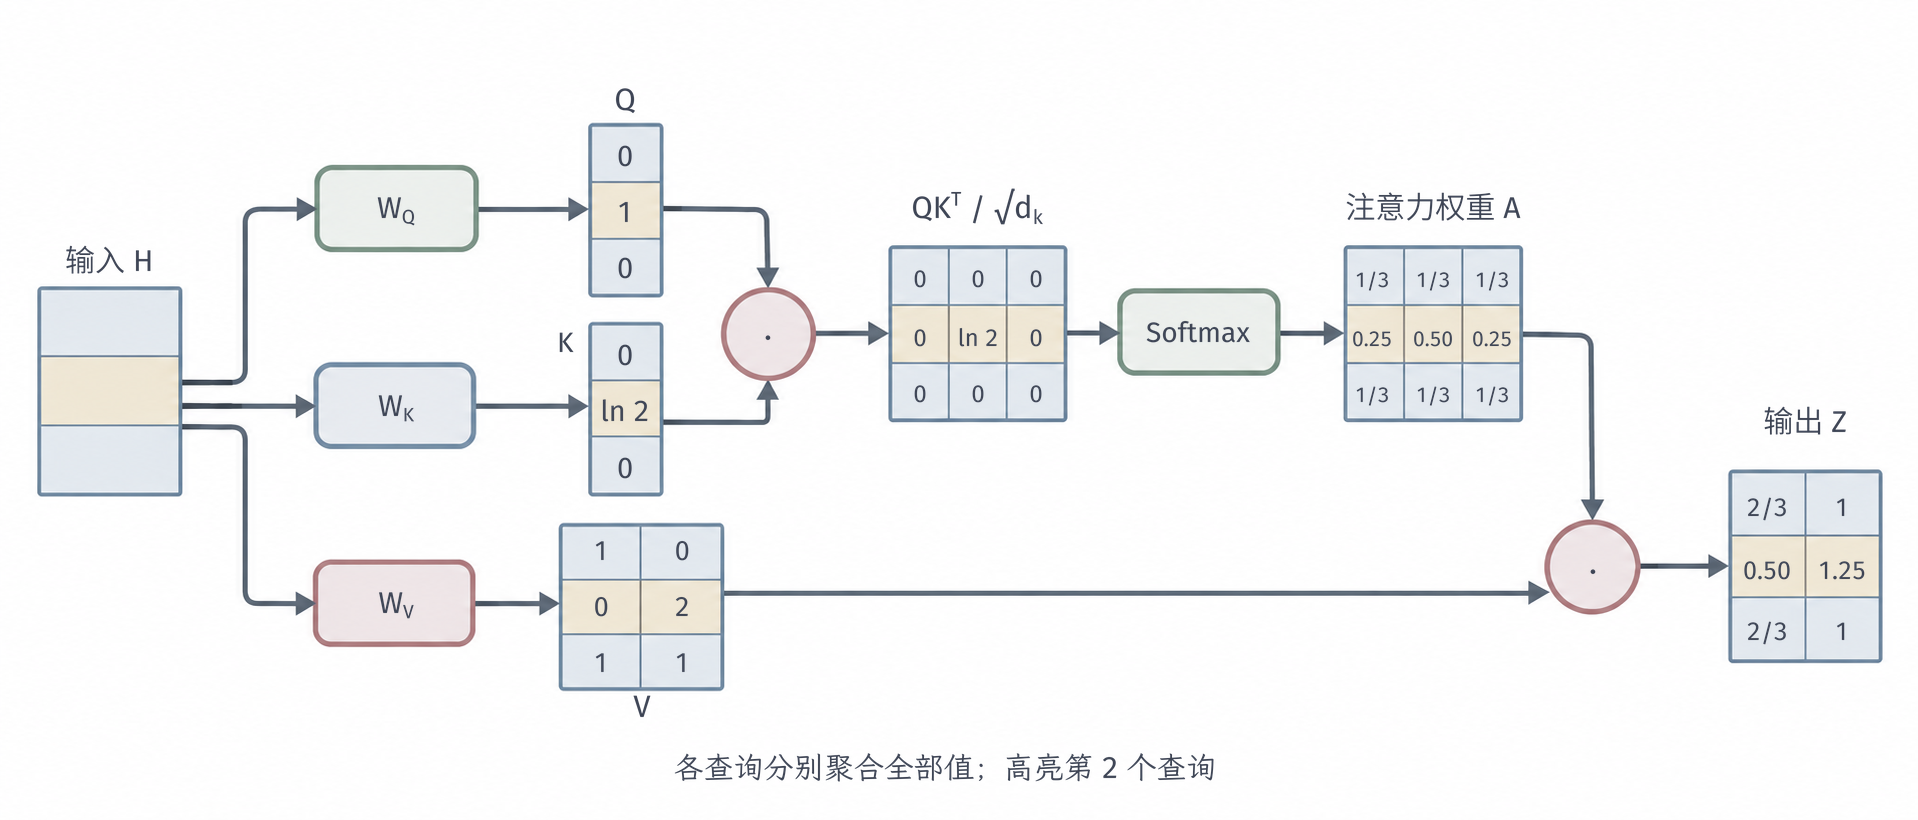
\includegraphics[width=162.391mm]{figures/05-neural-network-models/00-shared/generated/transformer-attention/figure.png}
  \caption{三个位置的缩放点积注意力，突出显示“追”这一查询。输入分别经三组投影产生查询$\bm Q$、键$\bm K$和值$\bm V$，三者各行依次对应猫、追、狗。突出显示的查询为$q_2=1$，与全部键匹配得到三个得分。Softmax按查询行产生权重矩阵，随后与值矩阵相乘得到各行输出；突出显示的一行权重为$(0.25,0.50,0.25)$，输出为$\bm z_2^{\top}=(0.50,1.25)$。浅色单元格示意矩阵数据，强调色标明同一查询的评分、权重与输出；$d_k=1$、$d_v=2$，数值均为教学设定。}
  \label{fig:transformer-attention}
\end{figure*}


\subsubsection{自注意力：同一序列内部读取}

上下文理解需要让一个输入位置结合其他输入位置。自注意力在式\eqref{eq:transformer-qkv}中取$\bm H_{\mathrm q}=\bm H_{\mathrm s}=\bm H$，查询、键和值都由同一组位置投影，得分矩阵为$n\times n$。

在看具体计算前，先回答一个自然的疑问：既然查询、键、值都来自同一序列，为什么还要用三组不同的投影，而不是让每个位置只带一个向量、自己跟自己点积？原因在于同一个位置在一次读取中要同时扮演三种角色。当它发起读取时，需要一个“我在找什么”的向量（查询）；当它被别人评估时，需要一个“我能提供什么线索”的向量（键）；被选中之后，真正传递出去的内容又是另一个向量（值）。一个位置发起查询时关心的特征，和它作为候选时值得被匹配的特征，以及它实际携带的信息，往往并不相同。三组独立可学习的投影，正是把这三种职责拆开，让训练分别调整“怎么找、怎么被找、给出什么”。因此三组投影各有参数；即使共享输入，通常也有不同的查询、键和值，只有特定参数设置才会得到$\bm Q=\bm K=\bm V$。为使三组线性投影可以逐项核对，图中取教学输入$\bm H=\bm I_3$，三组投影矩阵分别取为图示的$\bm Q$、$\bm K$、$\bm V$；独热输入让投影矩阵的每一行可直接对应图示数值，真实词元则通常使用前面定义的内容与位置表示。图~\ref{fig:transformer-self-attention}单独展开“追”的查询：三个位置提供值，按对应权重合成输出。中图权重表按查询位置排列，第2行就是$(0.25,0.50,0.25)$。若同一组键对应的另外两个查询取$q_1=\log_2 3$、$q_3=-1$，就分别得到第1行$(0.2,0.6,0.2)$和第3行$(0.4,0.2,0.4)$。查询不同，即使候选键值相同，读取也可以不同。整段输入可见时，各有效位置都在候选集合内，具体读取比例仍随查询与键改变。

\begin{figure*}[htbp]
  \centering
  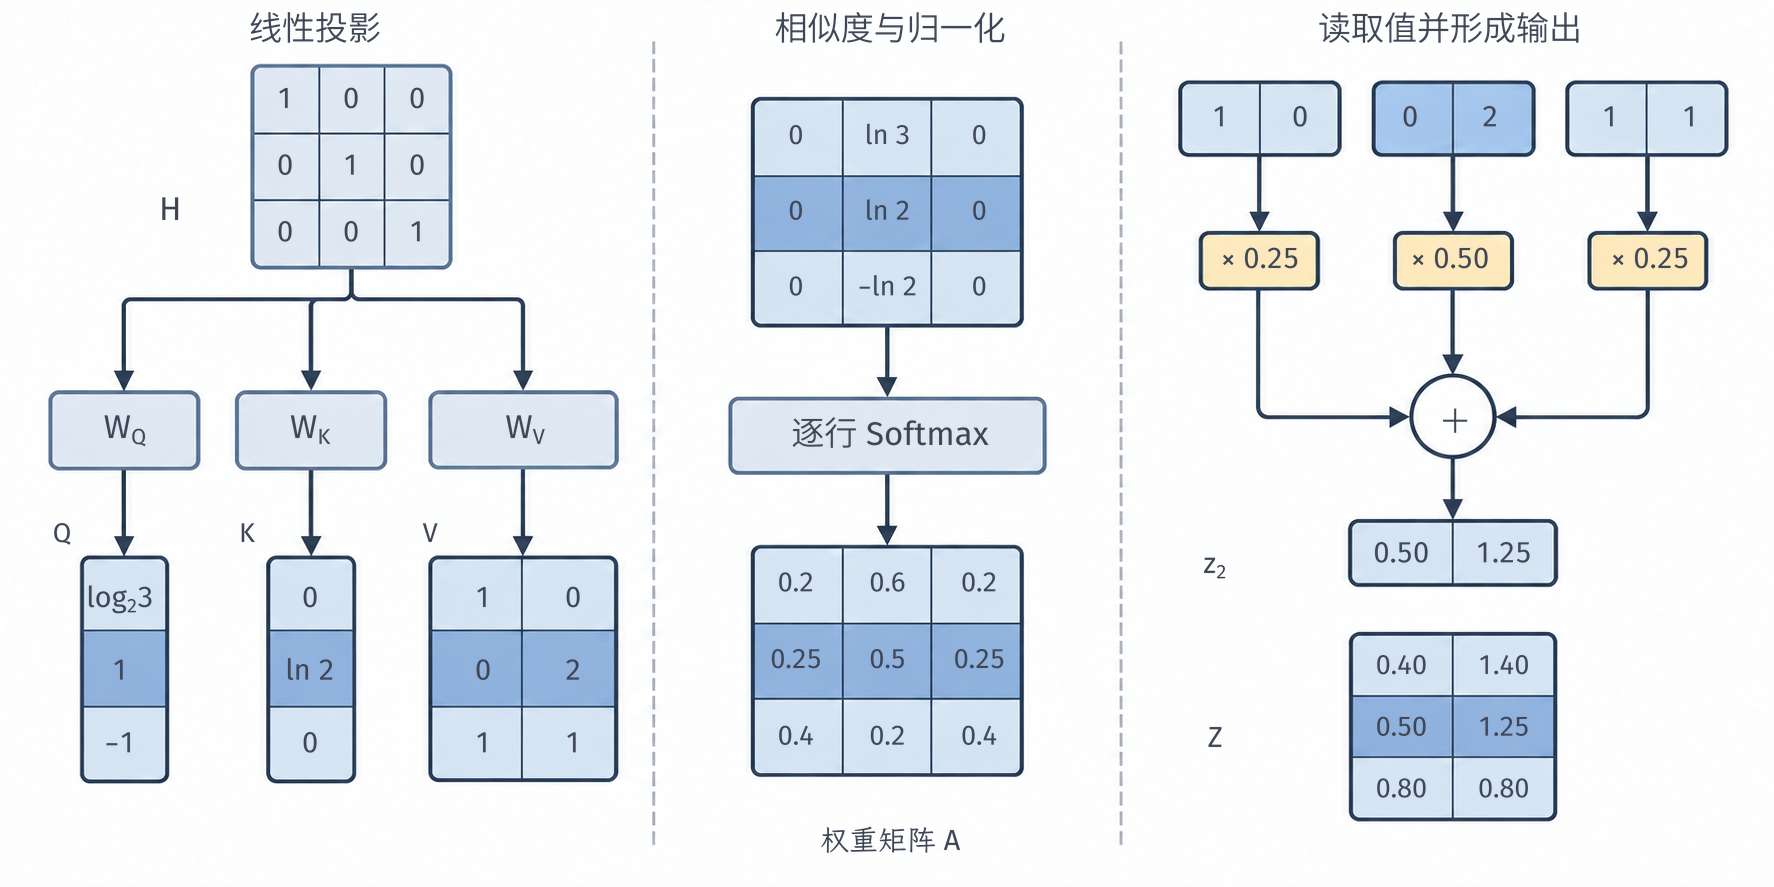
\includegraphics[width=150.199mm]{figures/05-neural-network-models/00-shared/generated/transformer-self-attention/figure.png}
  \caption{同一序列“猫／追／狗”上的自注意力。左图将教学输入$\bm H=\bm I_3$分别投影为查询、键和值；中图展示得分及逐行Softmax，行对应查询位置，列对应被读取位置。右图展开第2个查询，将三个二维值按$(0.25,0.50,0.25)$加权，得到$\bm z_2^{\top}=(0.50,1.25)$；下方矩阵汇总各查询分别计算的输出。$d_k=1$、$d_v=2$，所有数值为教学设定。}
  \label{fig:transformer-self-attention}
\end{figure*}

\FloatBarrier
\subsubsection{交叉注意力：从另一组表示读取}

目标序列需要读取源序列时，双方长度和职责通常不同。\term{交叉注意力}（cross-attention）让$\bm H_{\mathrm q}$提供查询，另一组$\bm H_{\mathrm s}$提供键和值，得分矩阵为$n_q\times n_s$。例如翻译目标当前位置用自己的状态提出查询，读取已编码的源句；每个查询产生一行输出，被读取侧提供键和值。以翻译“猫／追／狗”为例，图~\ref{fig:transformer-cross-attention}同时展开两个已知目标输入位置BOS和cat。BOS位置的输出用于预测cat，cat位置的输出用于预测chases；这两个目标状态产生两行查询，三个源编码状态产生三行键和值。源、目标长度不同，输出仍按目标查询排列，因此$\bm A$为$2\times3$，而$\bm Z$只有两行。

为了逐项算出一次交叉读取，取$d_k=1$，设目标投影后的查询为$\bm Q=(0,1)^{\top}$，源投影后的键为$\bm K=(0,\ln8,0)^{\top}$，值沿用前例的三个二维向量。BOS的三个得分都为0，Softmax给出$(1/3,1/3,1/3)$；cat的得分为$(0,\ln8,0)$，取指数得到$(1,8,1)$，归一化后为$(0.1,0.8,0.1)$。两行分别乘以同一个$\bm V$，得到$\bm z_1=(2/3,1)^{\top}$和$\bm z_2=(0.2,1.7)^{\top}$。后者对应cat发起的查询，供该目标位置后续预测使用。这一教学构造演示连续加权；真实翻译权重由训练形成，可能同时读取多个源位置。交叉注意力也可用于一种模态读取另一种模态；信息来源改变，不要求评分公式改变。

\begin{figure*}[htbp]
  \centering
  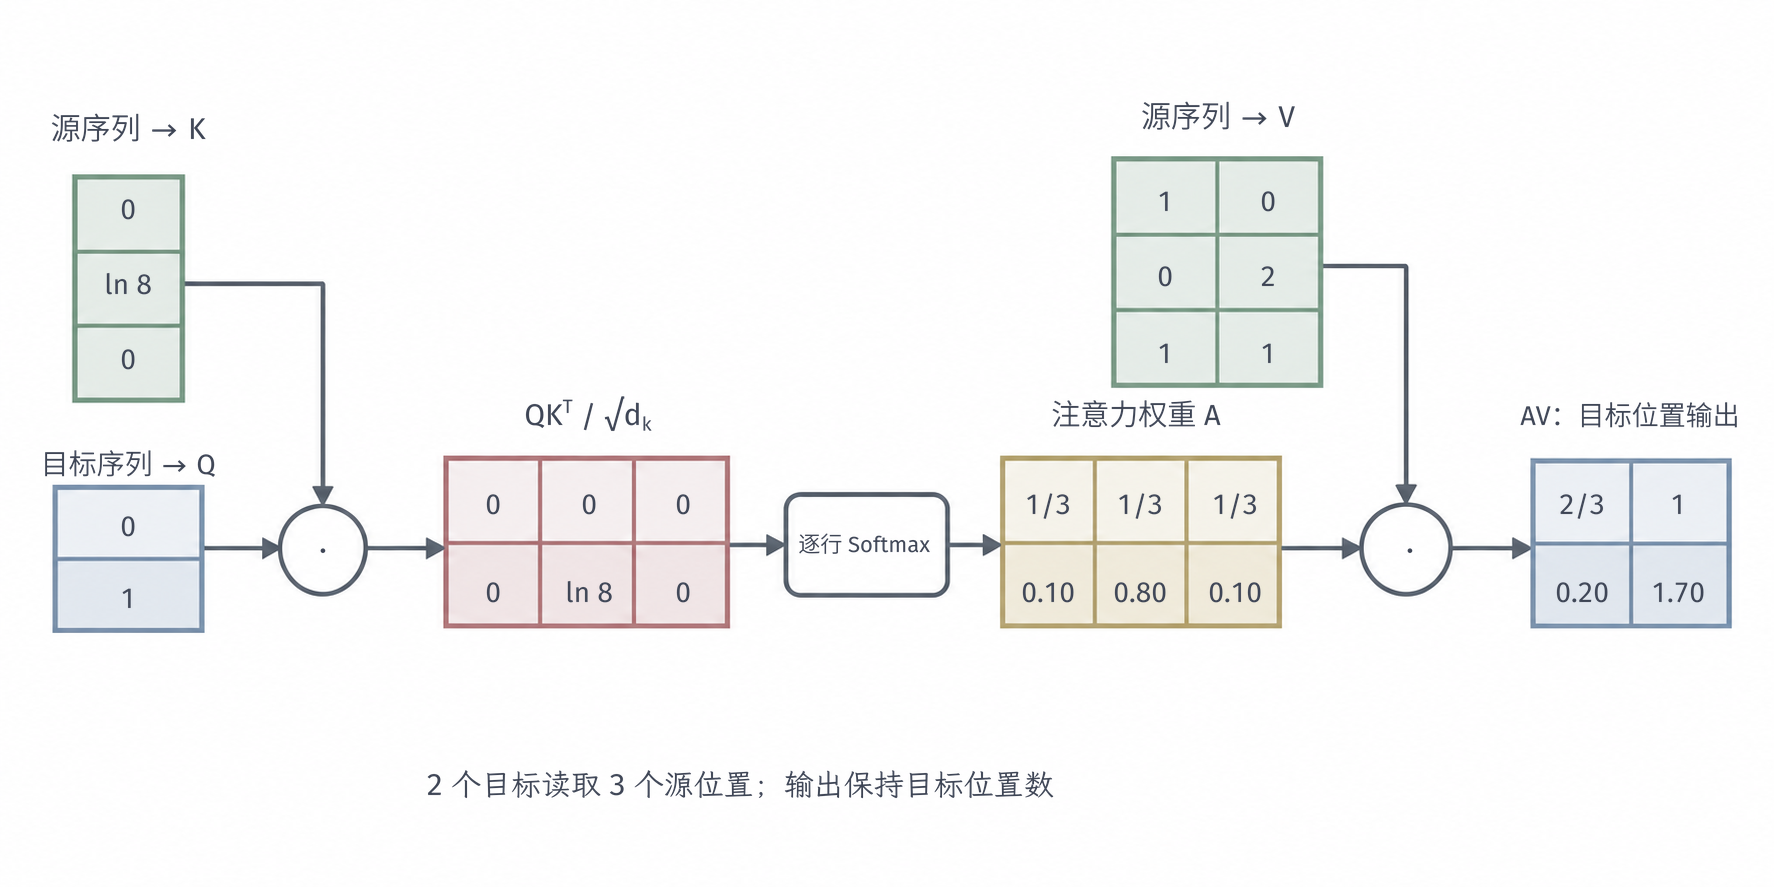
\includegraphics[width=150.199mm]{figures/05-neural-network-models/00-shared/generated/transformer-cross-attention/figure.png}
  \caption{两条不同序列的交叉注意力。目标输入BOS／cat的状态投影为两行查询，源输入猫／追／狗的编码状态分别投影为三行键和值。得分与权重矩阵的行对应目标查询、列对应源词元，因此形状均为$2\times3$；权重矩阵乘以$3\times2$的值矩阵后，输出为$2\times2$。较深的单元格突出cat这一目标位置从查询、评分、归一化到输出的对应关系。$d_k=1$，所有投影数值均为教学设定。}
  \label{fig:transformer-cross-attention}
\end{figure*}

交叉读取还说明了为什么输出长度跟随查询侧。假如只需要预测一个目标词，就只有一个目标查询，但它仍可读取全部源位置；源句变长会增加这一行的候选项，不会增加本步输出的行数。反过来，训练时同时提供多个目标查询，只是把多次读取排成多行，各行的权重仍分别归一化。源词与目标词因而不需要一一对应，一个目标词可以综合多个源位置，同一源位置也可以参与多个目标词的预测。

\subsubsection{因果注意力：只读取已知前缀}

同一序列也可能包含尚不能用于当前预测的未来内容。这个约束在逐词生成时是硬性的：预测第$i$个词时，第$i$个词本身以及它之后的内容还不存在，若网络在训练时“偷看”到了答案，学到的就不是据前缀预测，而是直接抄写。\term{因果注意力}（causal attention）通常指带因果掩码的自注意力，规定位置$i$只能读取$j\leq i$的键值，用结构保证这种泄漏不可能发生。图~\ref{fig:transformer-causal-attention}把“猫／追／狗”的可见范围直接排成矩阵。更新“追”时，“狗”所在格被屏蔽；“追”的输出经后续计算用于预测“狗”，因此输入位置和预测标签正好错开一步。它改变候选集合，投影与聚合公式仍为式\eqref{eq:transformer-attention}。训练把真实序列同时放入矩阵，各层的因果掩码共同保证前缀条件。前层若读取未来，后层接收到的表示已含未来内容，最后一层的掩码无法逆转这份混合。

\begin{figure*}[htbp]
  \centering
  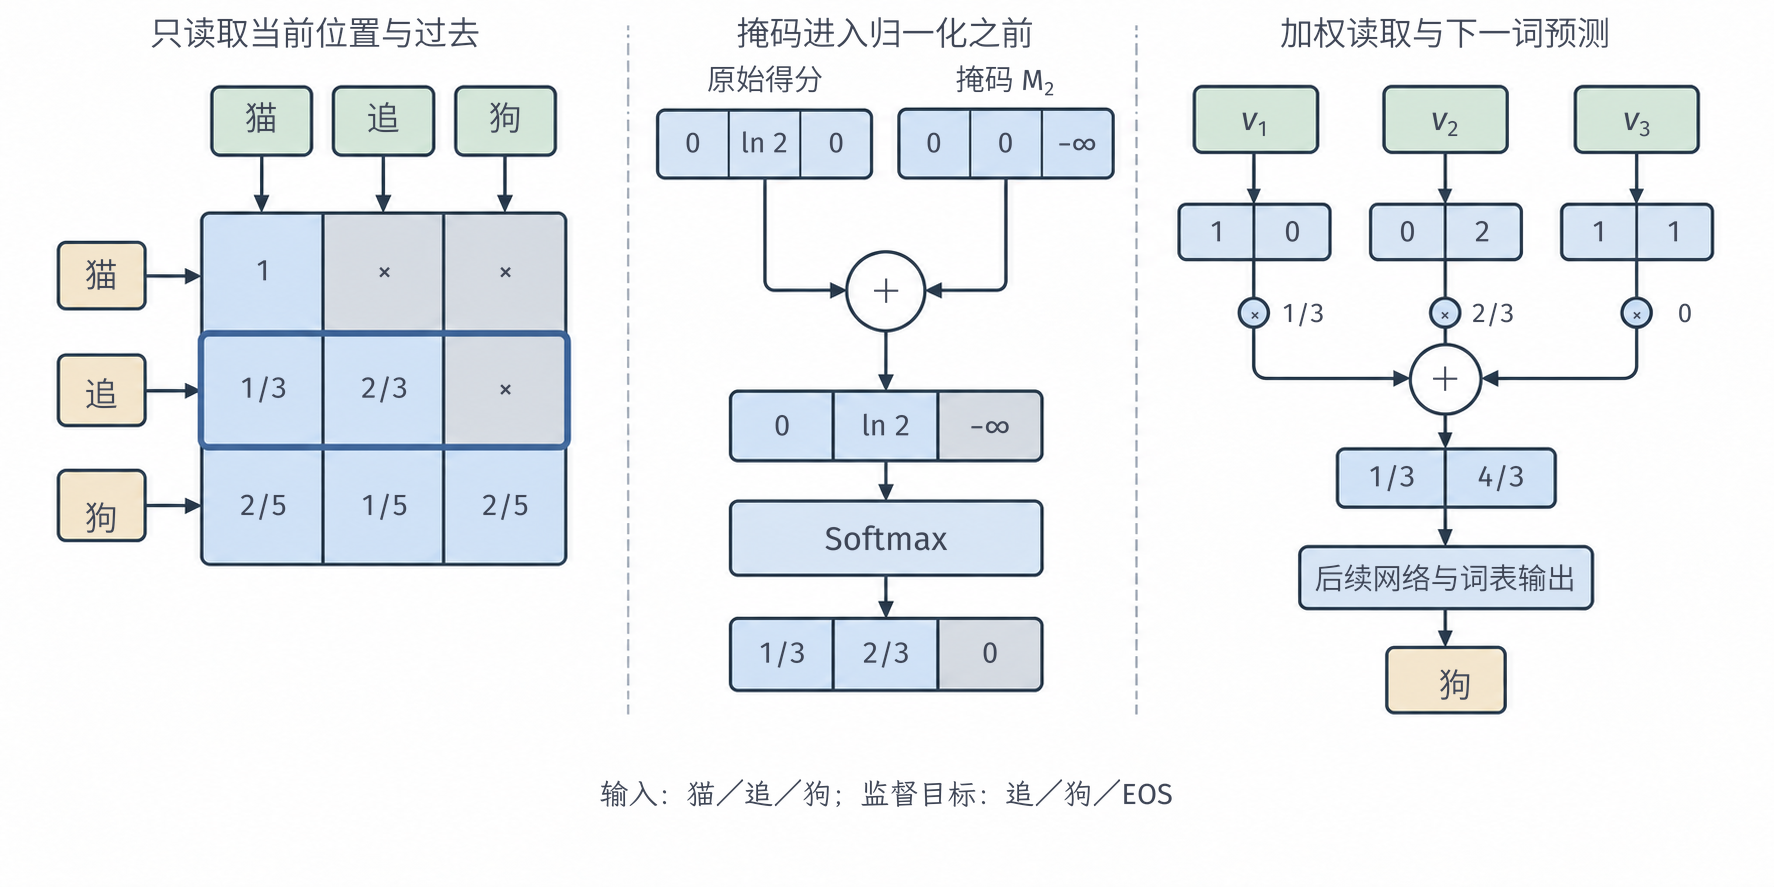
\includegraphics[width=150.199mm]{figures/05-neural-network-models/00-shared/generated/transformer-causal-attention/figure.png}
  \caption{“猫／追／狗”的因果自注意力。左图的行对应查询位置，列对应被读取的键；着色格给出可见位置的示例权重，浅灰叉号表示未来位置的权重为0。中图展开“追”这一行：原始得分先加因果掩码，再经Softmax得到$(1/3,2/3,0)$。右图加权读取值，得到$(1/3,4/3)^{\top}$，再经后续网络与词表头形成下一词元的预测分布；图中标出该位置的监督目标“狗”。预测“狗”时只读取当前已经给定的“猫／追”。底部展示错开一步的输入与监督目标，EOS为结束符；数值为教学设定。}
  \label{fig:transformer-causal-attention}
\end{figure*}
\term{填充掩码}（padding mask）阻止有效查询读取填充键；因果掩码排除未来位置。两者可以合并，前者排除不存在的输入，后者排除预测时尚不可知的信息。Softmax要求参与计算的查询至少有一个有效键；全行$-\infty$的指数归一化没有定义。填充查询可以跳过，也可以按有效规则得到随后弃用的输出，以便后续运算保持数值定义。因果掩码允许读取当前输入，这与预测下一个目标的移位配合，才构成没有目标泄漏的生成模型。

\subsubsection{多头注意力：并行形成不同的读取}

单组权重把各值压缩为一个混合。这会带来一个潜在问题：当一个位置需要同时关注几类性质很不同的信息时，单组权重被迫做一次性折中，混合后的向量里各类线索彼此纠缠，后续层很难再干净地分开。多头注意力的思路，就是并行地做几次关注点不同的读取，把各自结果原样保留下来再交由后续组合。\term{多头注意力}（multi-head attention, MHA）使用$h$组投影分别读取，再把结果拼接：
\begin{equation}
  \begin{aligned}
    \bm Z_a&=\operatorname{Attention}(\bm Q_a,\bm K_a,\bm V_a),\\
    \bm C&=\operatorname{Concat}(\bm Z_1,\ldots,\bm Z_h),\\
    \operatorname{MHA}(\bm H_{\mathrm q},\bm H_{\mathrm s})
      &=\bm C\bm W_{\mathrm o}\text{。}
  \end{aligned}
  \label{eq:transformer-multihead}
\end{equation}
头编号$a\in\{1,\ldots,h\}$，$\bm C\in\mathbb R^{n_q\times hd_v}$，$\bm W_{\mathrm o}\in\mathbb R^{hd_v\times d}$。常取$d_k=d_v=d/h$，使总投影宽度固定。各头分别学习权重和值特征，输出投影再组合这些结果。某头形成什么信息选择，由训练和输入决定；头之间是否互补可以据实际响应检验。固定$d$时增加头数同时减小每头宽度，读取组数与每组特征容量之间形成取舍。

图~\ref{fig:transformer-multihead}展开同一序列上的两个注意力头。三个位置的表示只输入一次，再交给每个头各自的查询、键和值投影；不同的投影使各头能够形成不同的读取权重和值特征。每个头都输出三行向量，拼接时对齐相同位置，只扩展特征维。例如，“追”在两个头中的输出拼为$[\bm z_{2,1}^{\top},\bm z_{2,2}^{\top}]$，这一拼接只扩展当前行的特征维，序列位置数保持原样。输出投影$\bm W_{\mathrm o}$再混合这些特征。多头既可用于自注意力，也可用于交叉注意力；每头还可以施加因果或其他掩码。常见的生成模型因此可以同时采用因果约束、多头投影和自注意力。

\begin{figure*}[htbp]
  \centering
  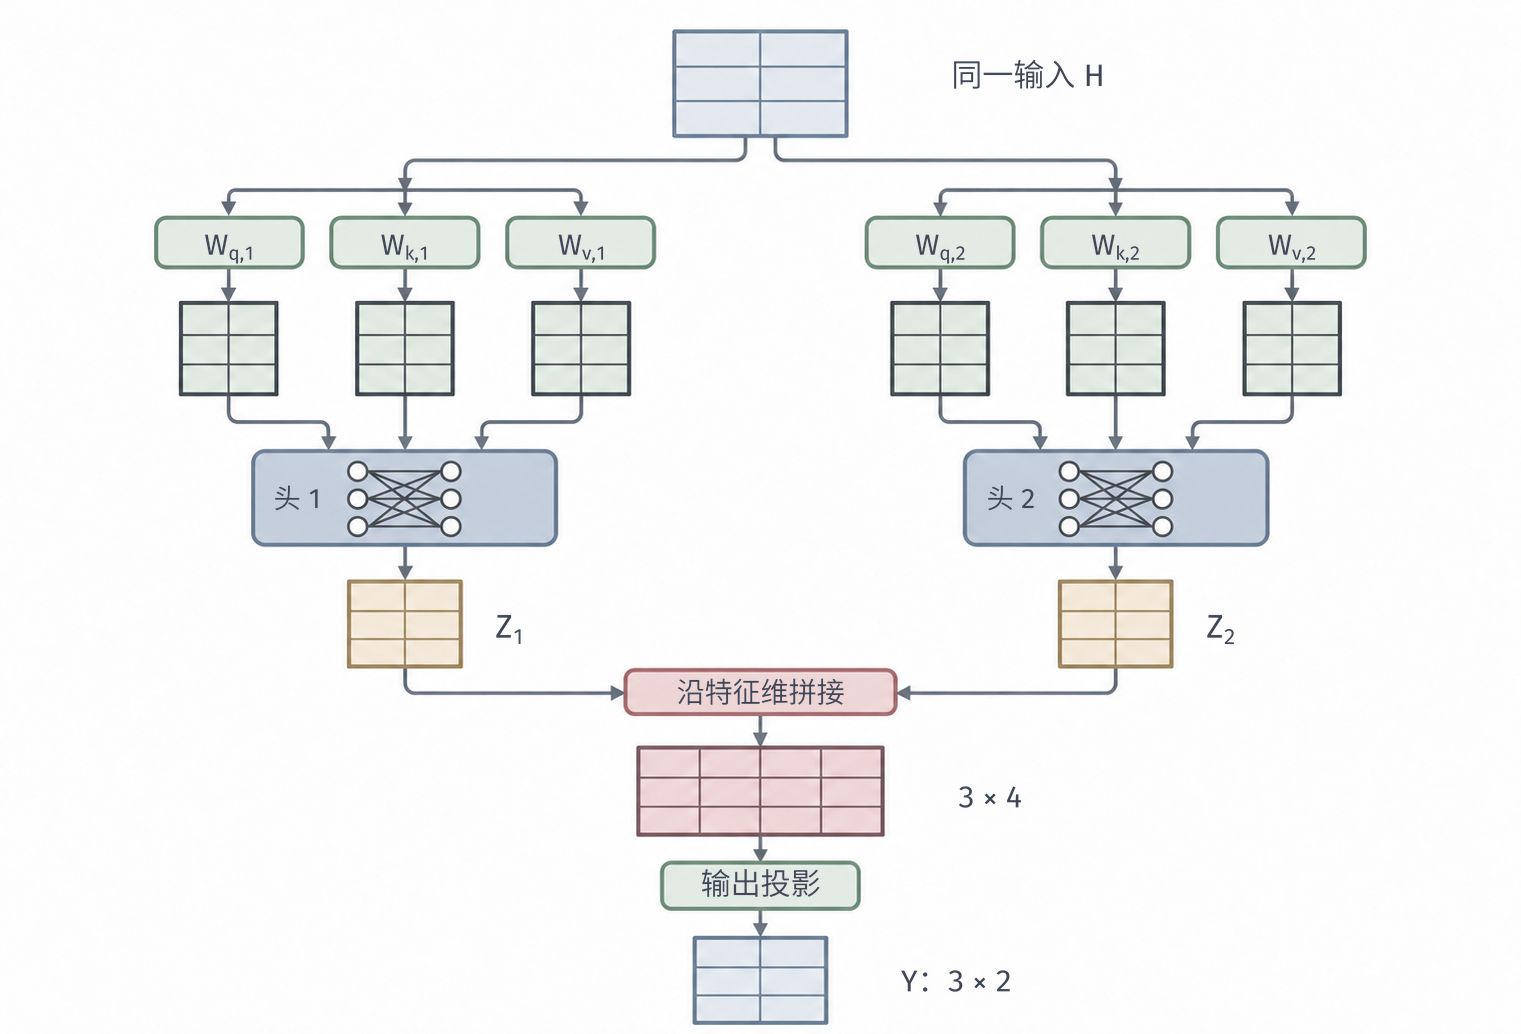
\includegraphics[width=128.778mm]{figures/05-neural-network-models/00-shared/generated/transformer-multihead/figure.png}
  \caption{同一输入序列上的两个注意力头。每个头分别学习$\bm W_{\mathrm q,a}$、$\bm W_{\mathrm k,a}$和$\bm W_{\mathrm v,a}$，独立完成评分、归一化和加权聚合，得到$\bm Z_a$。标有“沿特征维拼接”的框合并两路结果，两路输出的序列位置一一对齐，合并只增加特征宽度。拼接矩阵$\bm C$再经$\bm W_{\mathrm o}$投影，得到多头输出$\bm Y$。各头独立形成权重，输出投影组合它们的特征，具体信息分工由训练产生。}
  \label{fig:transformer-multihead}
\end{figure*}

可以把多头理解为先保留几份不同的读取结果，再决定怎样组合。假设两个头分别把“追”所需的主语线索和宾语线索读入不同特征，拼接保留了两组坐标，后续投影和FFN便可以对它们作不同处理。若先把两组结果平均为一个向量，这些差别可能在组合前就已丢失。这个例子说明多头结构提供的可能性；模型并没有预先为某个头规定“找主语”的职责，实际分工也可能重叠。

\subsection{前馈层}
\label{sec:transformer-feedforward}

注意力改变每个位置能读取什么，但读取结果还需转换为有用特征。这里要特别注意注意力本身做了什么、又没做什么：它本质上是对其他位置的向量做加权平均，只是把信息“搬运”并混合到当前位置，混合操作是线性的；若一个块里只有注意力，多层叠加所能表达的关系会受到很大限制。\term{逐位置前馈网络}（position-wise feed-forward network, FFN）补上的正是非线性加工这一环：它对每行单独使用同一组参数，先把特征投影到更宽的中间维度，在那里施加逐元素非线性、让不同特征相互组合，再投影回原来的隐藏宽度：
\begin{equation}
  \operatorname{FFN}(\bm H)
  =\phi(\bm H\bm W_1+\bm 1\bm b_1^{\top})\bm W_2
      +\bm 1\bm b_2^{\top}\text{。}
  \label{eq:transformer-ffn}
\end{equation}
其中$\bm W_1\in\mathbb R^{d\times d_f}$、$\bm W_2\in\mathbb R^{d_f\times d}$，$\bm b_1\in\mathbb R^{d_f}$、$\bm b_2\in\mathbb R^d$；$\bm 1$为$n$维全1向量，$\phi$逐元素作用。原始结构取$d_f=4d$并使用ReLU，其他结构可以采用第\ref{sec:ffn-activations}节介绍的激活函数和不同中间宽度。

每行使用同一FFN，输入内容和上下文不同，输出也随之不同。FFN在这一层不额外交换位置，它把已有上下文中的特征组合成新表示；下一次注意力再依据这些表示进行读取。若去掉非线性，两次仿射映射可以合成一次，扩张宽度本身就失去了增加非线性组合的作用。

这一层的参数量约为$2dd_f$，整段算术量为$O(ndd_f)$。长序列可能由位置对计算主导；短序列且$d_f$很大时，前馈计算和参数占比又会上升。完整成本需要同时计入注意力投影、聚合和前馈变换。

\subsection{残差连接与归一化}
\label{sec:transformer-residual-normalization}

层层变换时，可以让旧表示继续传递，同时学习需要增加的特征。这里遇到的是深层网络的普遍困难：若每个子层都必须把输入整体重写成输出，那么堆得越深，网络越难训练——梯度在层层连乘中容易放大或消失，而且多出的层至少不应把本来已经有用的表示改坏。\term{残差连接}（residual connection）把子层输出加到输入上，要求两者形状一致；这样每个子层只需学习在原表示之上“加一点什么”的增量，输入则保留一条畅通的直接传递路径，即使某层暂时学不到有用的东西，也可以把增量趋近于零、近似恒等地放行。注意力输出投影和FFN的维度恢复，也使这种相加可以在统一的$d$维空间进行。

不同位置的表示尺度还会影响点积和后续激活。随着层数叠加，表示向量的整体幅度可能逐渐变大或变小：注意力得分是点积，对幅度尤其敏感——若某些位置的向量范数很大，它们的点积会系统性地占优，Softmax便由幅度而非内容匹配主导，训练也容易失稳。\term{层归一化}（layer normalization, LayerNorm）在每个位置内部沿特征坐标计算均值和方差，不依赖其他样本或其他位置的统计量。之所以选择“沿一个位置自己的特征”统计，而不是像批归一化那样跨样本统计，是因为序列长度和批量大小经常变化、填充位置也不应参与，逐行归一化在训练和推理时都只依赖当前这一个位置，规则完全一致。对$\bm x\in\mathbb R^d$，令
\begin{equation}
  \begin{aligned}
    \mu(\bm x)&=\frac1d\sum_{k=1}^d x_k,\qquad
    s^2(\bm x)=\frac1d\sum_{k=1}^d(x_k-\mu(\bm x))^2,\\
    \operatorname{LN}(\bm x)
      &=\bm\gamma\odot
        \frac{\bm x-\mu(\bm x)\bm 1}{\sqrt{s^2(\bm x)+\varepsilon}}
        +\bm\beta\text{。}
  \end{aligned}
  \label{eq:transformer-layernorm}
\end{equation}
$\bm\gamma,\bm\beta\in\mathbb R^d$为可学习缩放和平移，$\varepsilon>0$避免分母为零，$\odot$表示逐元素乘法。应用于矩阵时按行计算，各位置共享$\bm\gamma,\bm\beta$。均值与方差只来自当前行，位置间模块再按任务掩码读取其他行\scite{ba2016layernorm}

原始Transformer把归一化放在残差相加之后，称为\term{后置层归一化}（post-layer normalization, Post-LN）。一个编码器块为
\begin{equation}
  \begin{aligned}
    \bm U^{(l)}&=\operatorname{LN}_{l,1}\!\left(
       \bm H^{(l-1)}+\operatorname{MHA}_l(\bm H^{(l-1)},\bm H^{(l-1)})\right),\\
    \bm H^{(l)}&=\operatorname{LN}_{l,2}\!\left(
       \bm U^{(l)}+\operatorname{FFN}_l(\bm U^{(l)})\right)\text{。}
  \end{aligned}
  \label{eq:transformer-postln-block}
\end{equation}
实际训练还可在子层输出加入Dropout，预测时关闭；这里省略它以突出确定性结构。\term{前置层归一化}（pre-layer normalization, Pre-LN）先归一化子层输入，再将子层输出加入原表示：
\begin{equation}
  \begin{aligned}
    \bm U^{(l)}&=\bm H^{(l-1)}+
      \operatorname{MHA}_l(\widetilde{\bm H}^{(l-1)},\widetilde{\bm H}^{(l-1)}),\\
    \widetilde{\bm H}^{(l-1)}&=\operatorname{LN}_{l,1}(\bm H^{(l-1)}),\\
    \bm H^{(l)}&=\bm U^{(l)}+
      \operatorname{FFN}_l(\operatorname{LN}_{l,2}(\bm U^{(l)}))\text{。}
  \end{aligned}
  \label{eq:transformer-preln-block}
\end{equation}
Pre-LN通常在整个堆叠末尾再归一化，之后交给输出层。图~\ref{fig:transformer-block}并列展开两种次序：Post-LN在残差相加后归一化，Pre-LN的跳跃路径则绕过归一化和子层；两者的学习性质将在第\ref{sec:transformer-normalization-extensions}节比较。同层各位置复用参数，后续层通常有自己的一组参数；额外的层间共享需要在模型中指定。

\begin{figure*}[htbp]
  \centering
  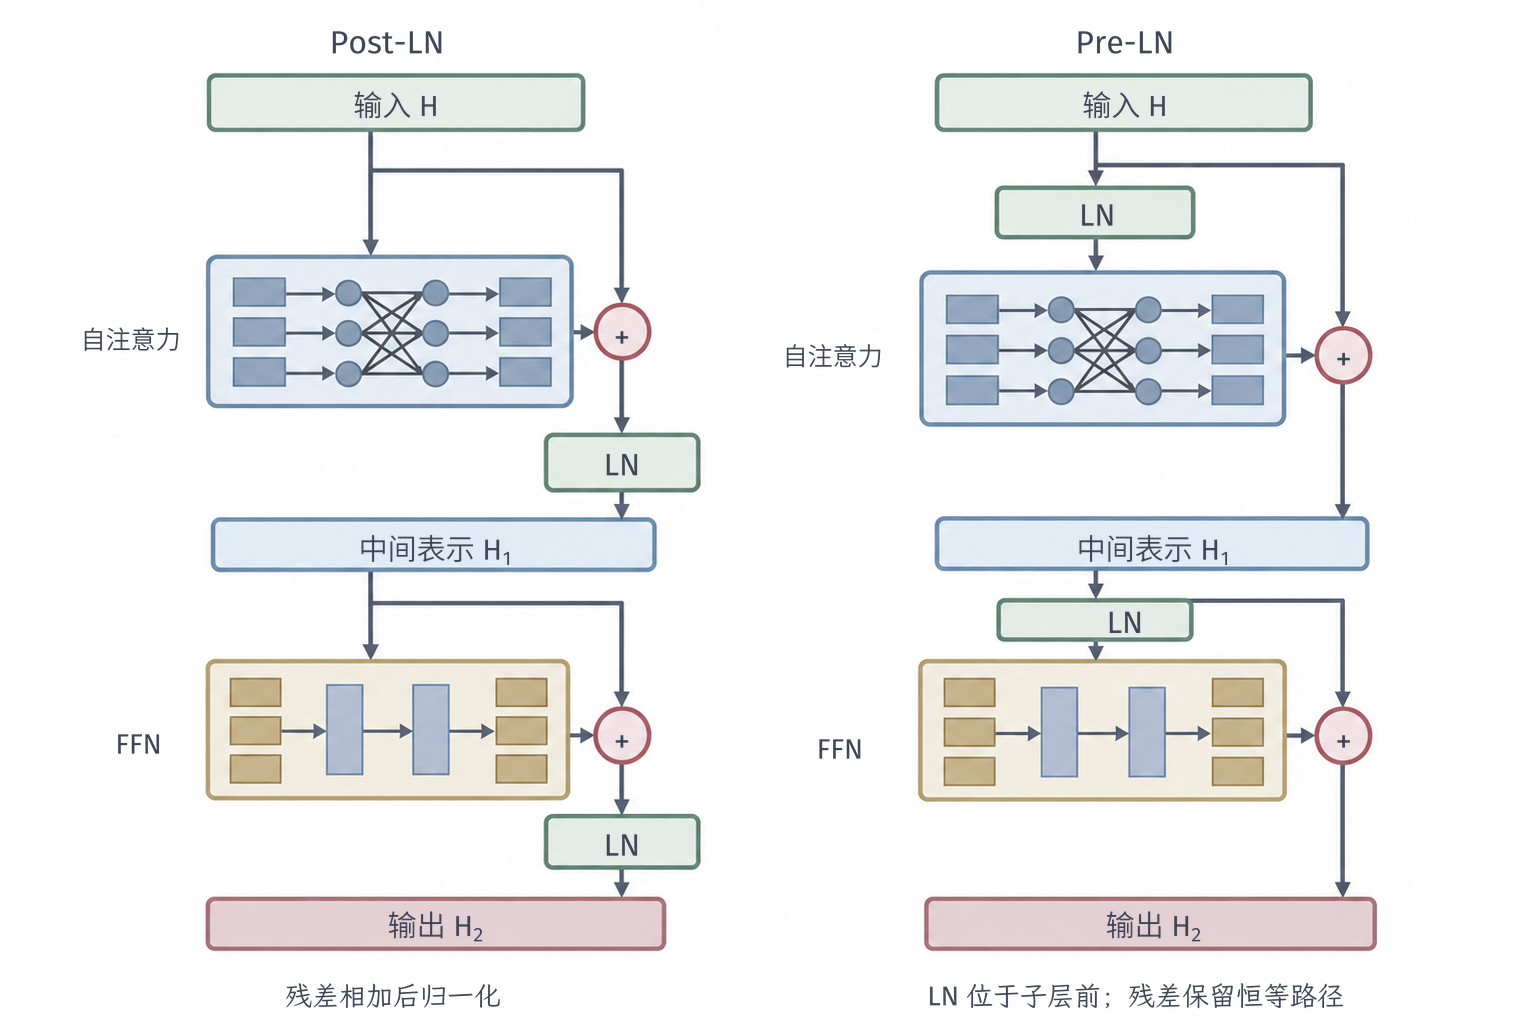
\includegraphics[width=128.778mm]{figures/05-neural-network-models/00-shared/generated/transformer-block/figure.png}
  \caption{Post-LN与Pre-LN编码器块的计算次序。输入与输出保持同一序列和特征形状。自注意力在行间交换信息，FFN分别变换各行；圆形$+$表示逐元素残差相加。图中箭头表示前向依赖；从残差路径可见，Post-LN的层间直达路径仍经过LN，Pre-LN则保留绕过归一化和子层的恒等支路。省略Dropout与Pre-LN堆叠末尾的归一化。}
  \label{fig:transformer-block}
\end{figure*}

\subsection{输出和网络架构}
\label{sec:transformer-architectures}

相同网络块可以用于不同预测过程，架构选择取决于输出对应哪些位置，以及这些位置在预测时能读取什么。在逐个认识模型之前，先抓住一个统一的判断方法：不要先记模型名字，而是先问两个问题——预测一个输出时，它被允许看到哪些位置（读取范围），以及损失落在哪一行表示上（监督位置）。整段分类只有一个答案，需要把$n$行汇成一个向量；词性标注每个词都有一个标签，损失落在每一行；翻译和续写下一个词尚未出现，必须因果读取。这三个问题一旦确定，编码器、解码器等“大块”如何摆放就基本确定了。\term{编码器}（encoder）通常让有效输入位置双向读取，形成整段上下文表示；\term{解码器}（decoder）在生成场景中使用因果自注意力，根据已知前缀预测后续输出。这里的“解码器”既可指原始编码器—解码器中的目标网络，也可指单独使用的因果网络，原始目标网络还读取源表示，单独因果网络则可以只读自身前缀。

\subsubsection{序列到分类或回归}

整段评论分类需要把$n$行表示转为一个向量。若最终输出表示为$\bm H$，有效位置集合为$V$，可以取$\bm r=|V|^{-1}\sum_{i\in V}\bm h_i$，再经分类头计算$\bm p=\operatorname{softmax}(\bm W_{\mathrm c}\bm r+\bm b_{\mathrm c})$。若有$c$类，$\bm W_{\mathrm c}\in\mathbb R^{c\times d}$，目标为$-\log p_y$。回归则用线性或受约束输出头形成数值，并选择与误差含义相符的损失。

另一种方式是在输入中加入专用读出词元，例如CLS，使用其末层表示$\bm r$。专用位置通过注意力读取整段，其输入参数、网络变换和任务头共同学习汇总方式。平均池化显式对位置等权，专用读出位置允许网络学习汇总，两者都要保证只读取任务允许的上下文。

\subsubsection{同步序列到序列}

词性或实体标签与输入位置对齐，可以对每行使用共享分类头，得到$\bm p_i$，在有效监督位置上计算平均交叉熵。离线标注可以读取完整输入；在线预测则需要因果掩码，或明确规定可等待多少后续位置。若预测下一时刻数值，目标还需移位。逐位置标签规定输出与输入的对应；离线、在线或有限延迟条件再规定每个输出可读的范围。

\subsubsection{异步序列到序列}

机器翻译的目标长度和源长度不同。\term{编码器—解码器}（encoder--decoder）先形成源表示$\bm H_{\mathrm s}$，目标网络在每层执行因果自注意力、交叉注意力和FFN。目标查询由该层已有的目标表示产生，键和值由最终源编码表示投影；源端填充掩码与目标端因果掩码分别约束两类读取。源表示供每个目标层重复读取，不必随着目标步重新编码；后文图~\ref{fig:transformer-architecture-original}用原始Transformer的翻译例子展示这条信息流。

给定源序列$x$，目标为$y_1,\ldots,y_m$，并将EOS计入目标，则条件分解为
\begin{equation}
  \begin{aligned}
    p_{\bm\theta}(y\mid x)
      &=\prod_{i=1}^{m}p_{\bm\theta}(y_i\mid x,y_{<i}),\\
    \ell(x,y)&=-\frac1m\sum_{i=1}^{m}
          \log p_{\bm\theta}(y_i\mid x,y_{<i})\text{。}
  \end{aligned}
  \label{eq:transformer-conditional-loss}
\end{equation}
$\bm\theta$包含输入、网络块和输出层参数。\term{教师强制}（teacher forcing）在训练时把真实目标前缀送入网络；目标输入是BOS、$y_1,\ldots,y_{m-1}$，目标标签是$y_1,\ldots,y_m$。全段输入已知，各位置可以并行计算，因果掩码保证第$i$个输出没有读到待预测的$y_i$。

条件生成也可用单个解码器：把源输入、分隔符和移位目标组织成同一序列，通常只在目标预测位置计算损失。使用全因果掩码时，源位置也只能读取其前缀；使用前缀掩码时，源位置可互相读取，目标位置可读取全部源前缀和此前目标。两种掩码都能服务于条件生成，源端表示的形成范围却不同。独立编码器—解码器另有源堆栈和交叉读取，三个计算组织应据各自依赖比较。

\subsubsection{序列续写与生成}

单独的因果解码器省略源交叉注意力，将已有文本本身作为条件。对词元$u_1,\ldots,u_n$，从BOS开始预测时，联合概率为$\prod_{i=1}^n p_{\bm\theta}(u_i\mid u_{<i})$。若最终表示$\bm h_i$对应第$i$个已输入词元，则下一词元概率为
\begin{equation}
  \bm p_{i+1}=\operatorname{softmax}
     (\bm W_{\mathrm{out}}\bm h_i+\bm b_{\mathrm{out}})\text{，}
  \label{eq:transformer-vocabulary-head}
\end{equation}
其中$\bm W_{\mathrm{out}}\in\mathbb R^{v\times d}$。可令$\bm W_{\mathrm{out}}=\bm E$进行输入输出嵌入共享，这使输入取出的内容向量和输出评分共用参数，限制了两接口可以独立调整的自由度。大词表投影还会产生$O(dv)$的单位置计算。

生成从已知前缀开始，计算下一词元分布，按指定策略选择一个词元，将其加入输入，再继续，遇到EOS或最大生成长度停止。贪心每步取当前条件下概率最大的词元，整段概率还随后续条件变化；采样则按指定分布产生词元。训练损失、预测时的选择策略和实际任务评价需分别说明。编码器适合已知完整上下文的理解，因果解码器适合按前缀生成，编码器—解码器使源与目标表示分开组织；输入何时可见与计算预算共同决定这些组织在实际任务中的适用范围。

\subsection{常见Transformer架构}
\label{sec:transformer-common-architectures}

前面按输出形式组织了网络，这里进一步比较几种实际模型。读这一节时容易陷入“背模型配置”的误区，更有价值的读法是把它们看成同一组构件在“读取范围＋预训练目标”两个维度上的不同选择：它们的注意力、FFN、残差几乎相同，真正不同的是允许每个位置读到什么，以及用什么任务在大规模无标注文本上预先训练。同样面对“猫追狗”，BERT可以补回被遮蔽的“追”，GPT可以根据“猫追”续写“狗”，编码器—解码器则可以把整句翻译成另一种语言。它们共享注意力与前馈计算，但读取范围、监督位置和生成过程不同。以下架构图沿用整序列的分层表示：长条作用于整段序列，虚线框表示重复堆叠，箭头表示前向信息依赖。BERT和RoBERTa另用公式展开一个Post-LN块，GPT则并列比较归一化次序。长条和块内公式分别说明词元读取与层间更新\scite{bishop2024deep} 各图都把中文例子按词划分，以便观察对应关系；这种教学划分不代表某个模型实际采用的子词分词器，图中的词元是监督目标或示例生成结果。

\subsubsection{原始Transformer：源与目标分开建模}

翻译时，源句通常已经完整给定，目标句却需要逐词产生。这两个条件不同，原始Transformer便用两组网络分别处理：编码器双向读取源句，解码器因果读取已有译文，再通过交叉注意力查询源表示。原论文基础模型的编码器和解码器各有6个块，隐藏宽度512，8个注意力头，FFN中间宽度2048，采用正弦位置编码、ReLU与Post-LN\scite{vaswani2017}

\begin{figure*}[t]
  \centering
  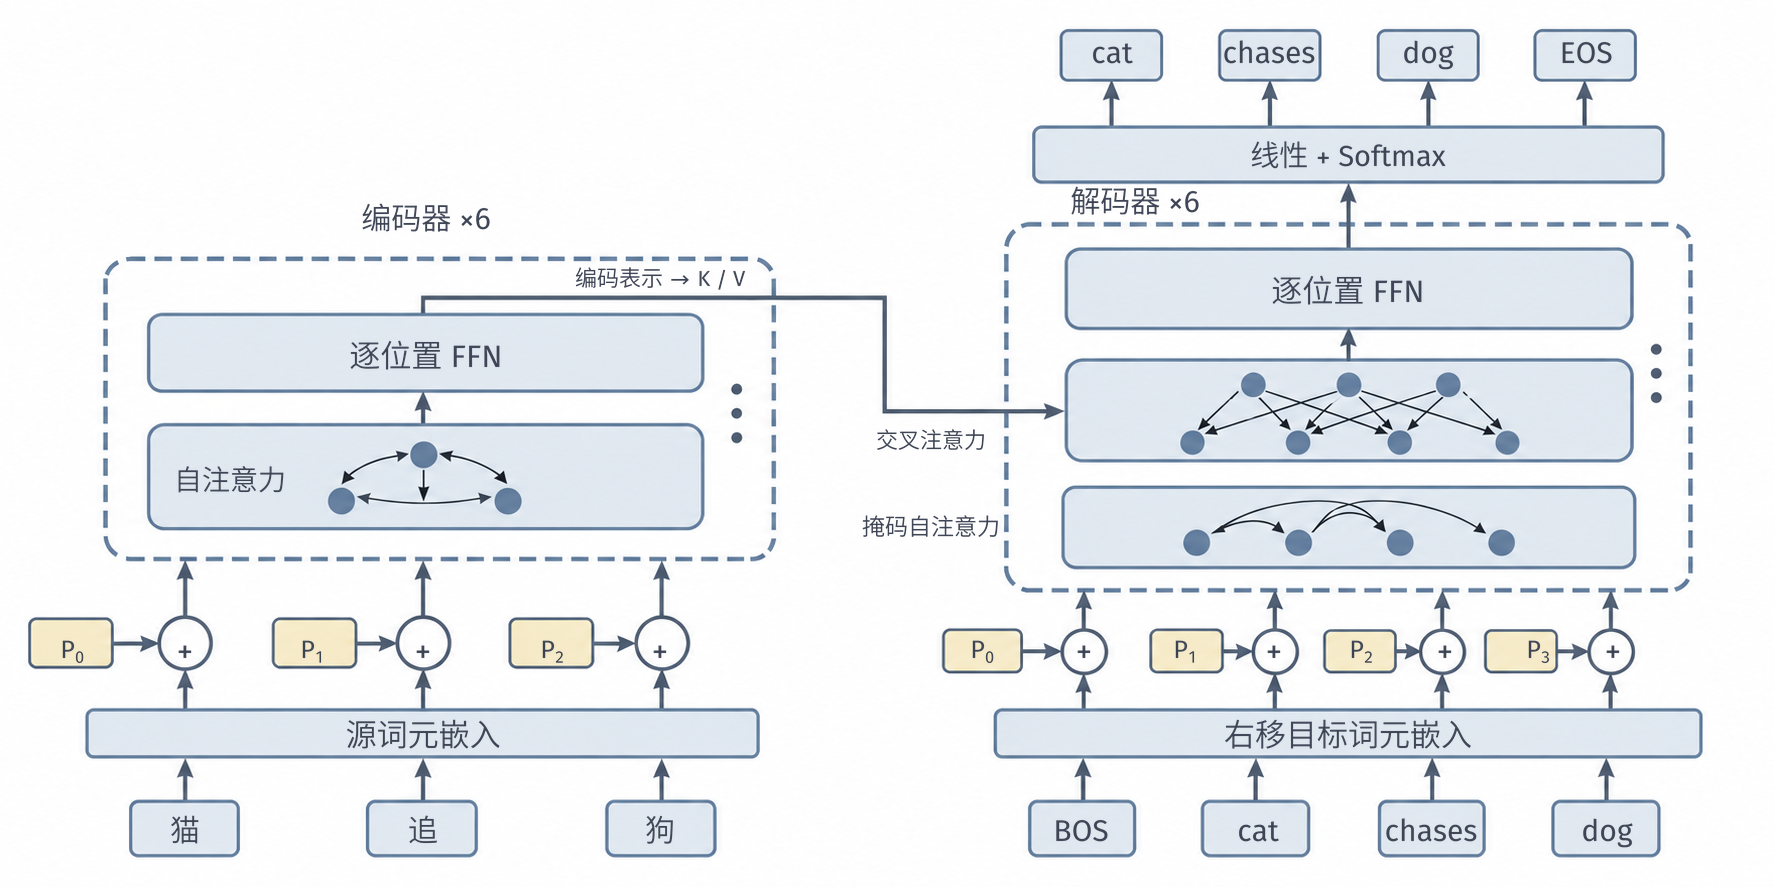
\includegraphics[width=150.199mm]{figures/05-neural-network-models/00-shared/generated/transformer-architecture-original/figure.png}
  \caption{原始Transformer基础模型的整网信息流。源编码器与目标解码器各堆叠6个块；每个长条作用于整段序列。解码器先因果读取目标前缀，再交叉读取最终源表示；各目标块据此生成K、V，Q来自各块的目标路径，不与同编号的中间编码层配对。目标输入右移，输出为对应的下一词元，最后预测EOS。省略残差、Post-LN、Dropout和嵌入缩放；结构依据Vaswani等（2017）。}
  \label{fig:transformer-architecture-original}
\end{figure*}

以“猫追狗”的翻译说明图~\ref{fig:transformer-architecture-original}的条件生成过程。训练时，解码器输入是右移的目标“BOS、cat、chases、dog”，对应监督目标是“cat、chases、dog、EOS”。预测dog的目标位置可以读取cat和chases，同时通过交叉注意力读取源句中的“狗”；“狗”的源词元属于已经给定的条件，目标词元dog则是这一位置需要预测的监督标签。推理时没有正确译文可供右移，解码器把自己已经生成的词元作为后续输入。

沿图中两条路径继续看，编码器输出的每一行已经结合源句上下文。源位置“狗”的表示不再只是词表中的“狗”，其中还可能包含它与“追”的关系。解码器也先用因果自注意力整理已经生成的目标前缀，再把这一层的目标表示用作查询。因此，交叉注意力读取的是“当前翻译状态需要什么源信息”，而不是直接拿一个孤立的英文词去查中文词表。查询随目标位置和网络层改变，源端最终表示则保持不变。

这里的“源表示保持不变”不表示所有解码器层共享同一套键和值。每个解码器层有自己的交叉注意力投影，将同一份最终源表示映射成该层的键和值；编码器的第1层也不会专门连接解码器的第1层。固定源句和模型参数后，各目标步复用每层各自的源投影。这样既能让不同层选择不同源特征，又能避免在每次生成时重新编码源句。

掩码可以用矩阵形状逐项核对。若源句有$n$个有效词元，移位后的目标输入有$m$个位置，则源自注意力的得分为$n\times n$，目标自注意力为$m\times m$，交叉注意力为$m\times n$。目标自注意力保留下三角，交叉注意力允许读取全部有效源位置；目标中尚未生成的词元不能通过第一条路径进入计算，完整源句则可以通过第二条路径参与预测。批量中的填充位置另行屏蔽，不计入这些有效长度。

参数学习最小化式\eqref{eq:transformer-conditional-loss}的条件负对数似然，编码器、解码器和词表头一起更新。教师强制允许并行计算所有目标位置，但生成时仍须逐步扩展前缀；训练用真实前缀而预测用自身输出，会使两种过程经历不同的输入分布。源投影和已有目标键值可以缓存，复用先前前向结果；新的目标词元仍在本步选择后进入下一步输入。

EOS也属于预测目标。以图中的译文为例，最后一个输入dog对应的标签为EOS，因此网络会学习在什么条件下结束，而不必让目标长度等于源长度。生成时若某一步选错了词，后续查询会沿错误前缀继续形成；训练时较小的单词预测损失，也不能保证逐步选择得到整段概率最大的译文。模型给出条件分布，解码方法再决定如何在这些分布上选择序列，两者需要分别评价。

源、目标长度还决定了两条路径各自的成本。固定隐藏宽度$d$，只统计一层的位置配对与聚合，源自注意力为$O(n^2d)$，目标自注意力为$O(m^2d)$，交叉注意力为$O(mnd)$。交叉项来自每个目标查询都要对$n$个源位置评分和读取；它不是源端平方项或目标端平方项的重复计算。实际整网还需乘上各自层数，并计入投影、FFN和词表输出；缓存减少重复工作，但不会让新查询免于读取所需源信息。

这种组织可以一次编码源句，并在多个解码步骤中复用源表示，源端也能充分结合左右语境，适合输入和输出边界明确的翻译、摘要等任务。代价是需要维护两组网络和交叉注意力；当任务只是从一个前缀继续写下去时，单一路径的因果模型通常更直接。成本比较还需固定源长、目标长、宽度和层数，两组堆栈及交叉注意力各占多少计算由这些配置决定。



\subsubsection{BERT：利用左右语境形成表示}

若目标是判断句意或标注每个词元，当前位置常常需要后文。\term{BERT}保留双向编码器，并使用\term{遮蔽语言模型}（masked language model, MLM）预训练：先扰动部分输入，再从上下文恢复原词元。例如输入“猫 [MASK] 狗”时，被遮蔽位置必须结合“猫”和“狗”预测“追”。原始BERT还通过CLS位置的表示预测两个句段是否相邻，即下一句预测（next sentence prediction, NSP）。BERT Base为12层、宽度768、12个头，Large版本为24层、宽度1024、16个头；输入叠加词元、可学习位置和句段嵌入，块内使用GELU与Post-LN\scite{devlin2019}

图~\ref{fig:transformer-architecture-bert}中，MLM只在选中的位置接受词元监督；用于分类时，则可以在CLS表示上接任务头。原始训练并非把每个选中位置都替换为[MASK]，还混合随机替换和保留原词，以减轻预训练输入与实际使用输入的差别。这里画出遮蔽分支，是为了突出双向上下文如何帮助恢复缺失内容。

\begin{figure*}[t]
  \centering
  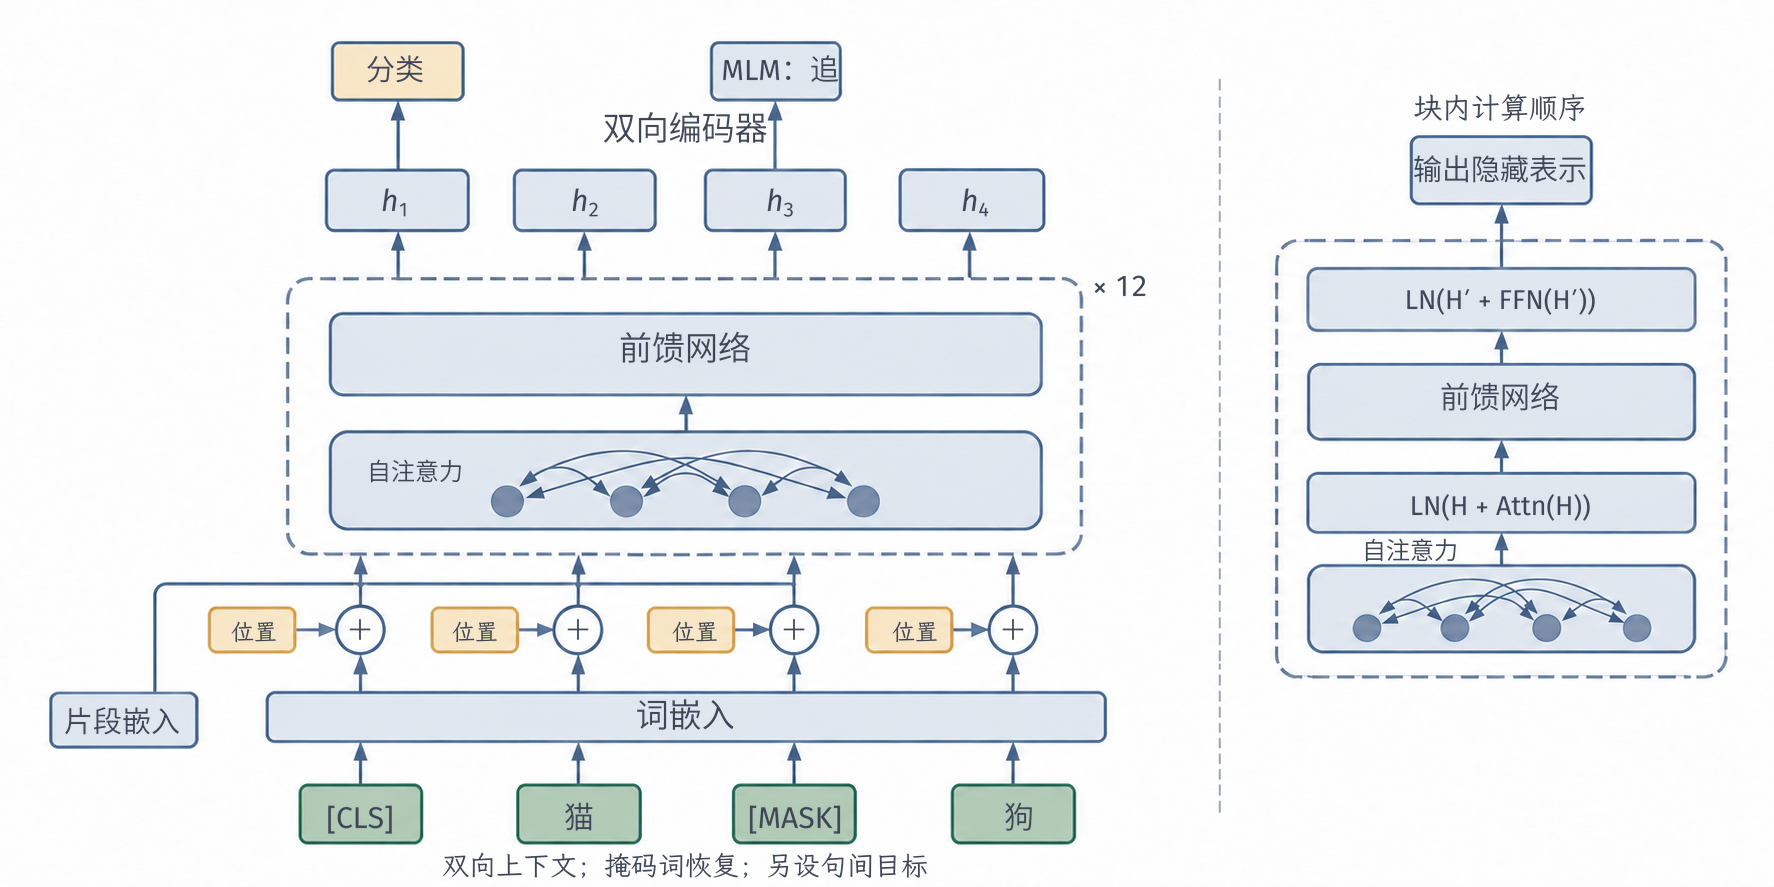
\includegraphics[width=150.199mm]{figures/05-neural-network-models/00-shared/generated/transformer-architecture-bert/figure.png}
  \caption{BERT Base的双向编码器与预测位置。词元、位置和句段嵌入相加，12个编码器块形成上下文表示；左侧画出一个短片段，省略分隔符。CLS用于序列分类，遮蔽位置由MLM头恢复“追”。主流程省略层内残差与归一化，右侧展开一个Post-LN块；$\operatorname{Attn}$、$\operatorname{FFN}$分别表示注意力与前馈变换，$\bm H'$表示注意力子层残差归一化后的输出。残差直接写入公式；省略Dropout与NSP头。结构依据Devlin等（2019）。}
  \label{fig:transformer-architecture-bert}
\end{figure*}

原始BERT随机选取约15\%的普通词元作为MLM监督位置，其中80\%改为[MASK]、10\%替换为随机词元、10\%保持原样。设选中集合为$M$、扰动输入为$\widetilde x$，词元损失为$-\sum_{i\in M}\log p_{\bm\theta}(x_i\mid\widetilde x)$；未选位置仍提供上下文，但不直接接受这项恢复监督。原始预训练还加上句段对的二分类损失。微调时换接任务头，使用任务标注继续更新编码器；冻结编码器只训练头则是另一种成本较低的使用方式。

微调所用的标签会改变信息汇总的方向。例如，判断“这部电影并不精彩”的情感时，CLS本身没有这句话的词义；它在多层自注意力中读取其他位置，分类损失再推动整个编码器保留与标签有关的线索。若改为给每个词元标注实体类型，就把监督接到各自的末层表示上。两种任务可以共享预训练参数，但读出位置与损失不同；预训练得到一个可供继续调整的表示起点，并未预先确定所有下游任务的分类规则。

双向读取使BERT适合在完整输入上做分类、抽取和序列标注；各位置表示可以在一次前向计算中并行形成。MLM按扰动输入恢复选中词元，定义了这种条件预测。自由续写还需要左到右或其他序列生成目标及对应解码过程。若当前位置读取了未经扰动的自身内容，恢复同一词元便有直接答案可用，因而目标和可见输入必须一起设计。



\subsubsection{RoBERTa：改进双向编码器的预训练}

BERT的效果还取决于预训练方式，而不仅是网络拓扑。\term{RoBERTa}保留BERT式双向编码器，主要改变训练配方：每次送入序列时重新抽取遮蔽位置，取消NSP，使用更大的批次、更多文本和更充分的训练，并改用字节级BPE词表。图~\ref{fig:transformer-architecture-roberta}沿用BERT式编码器，画出遮蔽“追”的一次训练输入；动态遮蔽表示不同次训练可以重新抽取遮蔽位置，让模型接触不同的上下文恢复问题\scite{liu2019roberta}

\begin{figure*}[t]
  \centering
  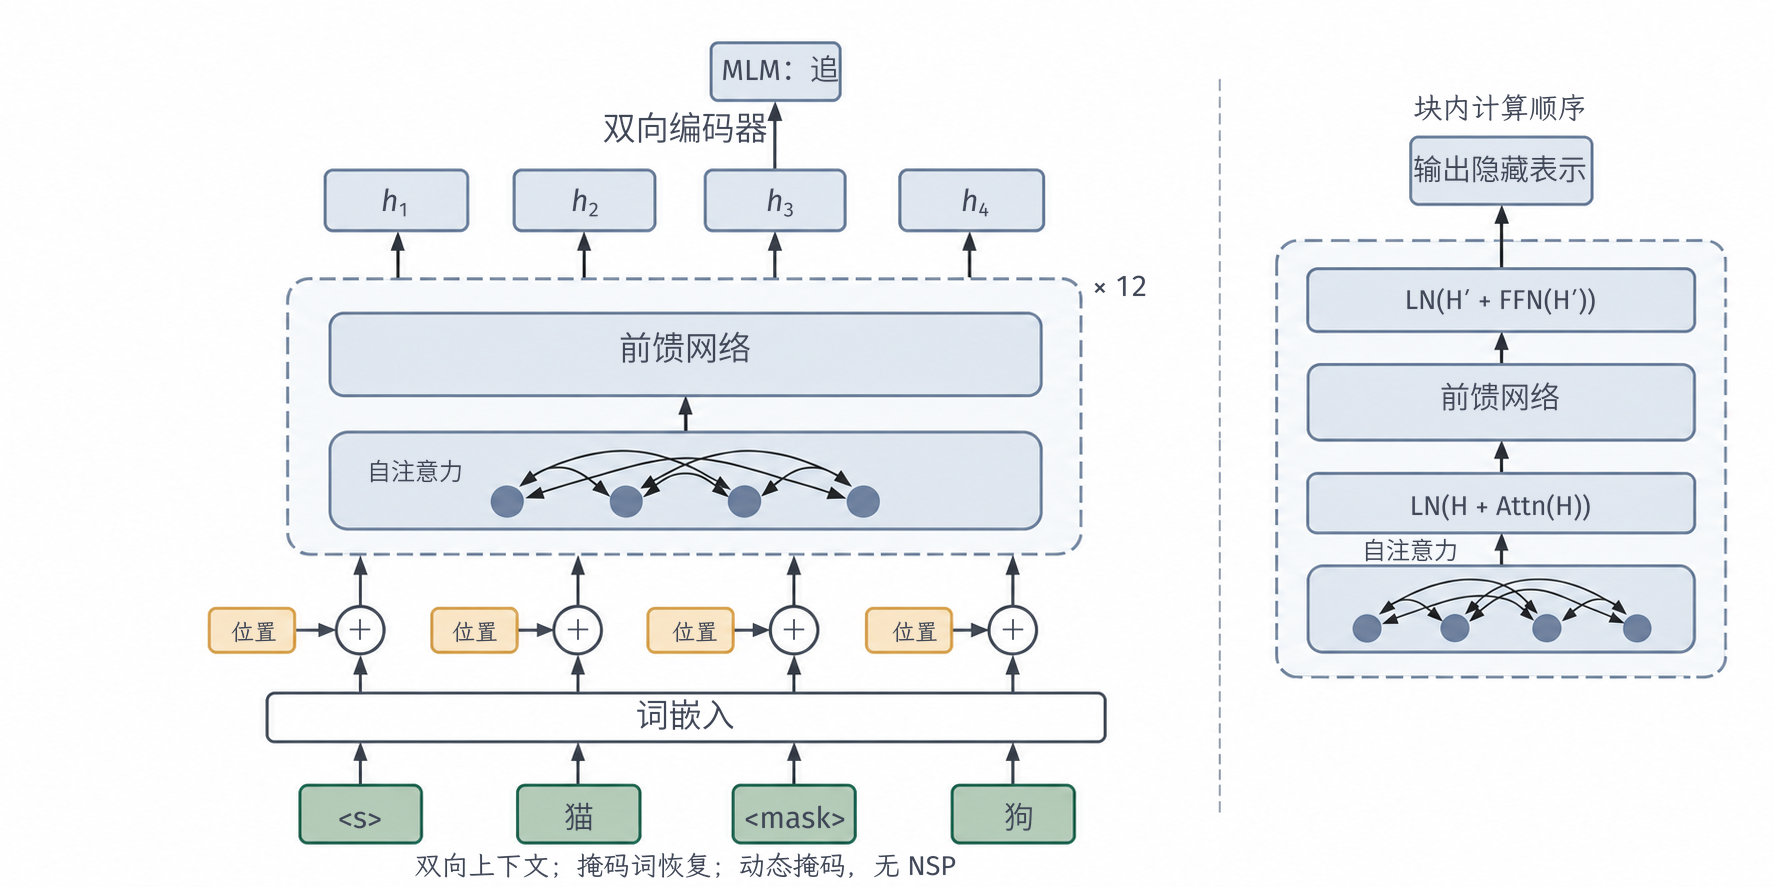
\includegraphics[width=150.199mm]{figures/05-neural-network-models/00-shared/generated/transformer-architecture-roberta/figure.png}
  \caption{RoBERTa Base的双向编码器与遮蔽恢复。词元与可学习位置嵌入相加，12个编码器块形成上下文表示，选中的遮蔽位置由MLM头恢复“追”。核心结构与BERT相同，预训练采用动态遮蔽且不使用NSP。主流程省略层内残差与归一化，右侧展开Post-LN计算次序；省略Dropout。训练差异依据Liu等（2019）。}
  \label{fig:transformer-architecture-roberta}
\end{figure*}

它仍在选中的位置计算MLM交叉熵，不同遮蔽样本通过同一网络分别前向；各样本内部双向读取，样本之间不交换词元。NSP是句段级训练目标，取消它改变了样本组织和损失；编码器内部的注意力模块保持原来的读取作用。下游分类或标注仍需把末层表示接到相应任务头，并明确哪些参数继续训练。

动态遮蔽改变的是什么，可以用同一句训练文本说明。一次输入“猫 [MASK] 狗”，要求恢复动作；另一次输入“[MASK] 追 狗”，要求恢复动作的发起者。底层词元序列相同，提供给网络的上下文和接受监督的位置却不同。于是，同一文本可以产生多种恢复问题。每次前向都需要按本次扰动重新计算双向表示，不能把上次遮蔽输入的中间结果直接当作这次的表示；图中展示的是其中一次扰动，而不是同时混合所有遮蔽结果。

RoBERTa以相同核心结构检验数据、目标与优化设置的作用。其预训练投入和方案同时变化，论文的整体收益应结合这些配置解释；单项改动的作用需要相应对照实验。两者在使用方式上仍然接近，都适合完整输入上的理解任务，也都需要额外设计才能作为自由续写模型。



\subsubsection{GPT：因果解码器及其版本演进}

续写时，模型只能依据已经出现的内容预测下一项。\term{GPT}家族由这一任务发展而来；早期公开的GPT-1、GPT-2和GPT-3都采用只有解码器的组织，每个块包含因果自注意力与FFN，没有独立源编码器，也没有连接源表示的交叉注意力。版本演进涉及块内计算、模型规模、训练目标和使用方式，以下分别说明它们改变的输入与参数。

\paragraph{GPT-1：建立预训练后微调的因果模型}

初代GPT于2018年采用12层、宽度768、12个头的结构，配合可学习绝对位置、GELU与Post-LN；先用下一词元预测进行语言模型预训练，再针对下游任务微调。为便于与后续版本区分，这里称其为GPT-1\scite{radford2018gpt}

图~\ref{fig:transformer-architecture-gpt}并列比较早期三个版本的计算次序。以词元序列说明监督：“猫”位置预测“追”，“追”位置预测“狗”。训练时三个位置可以一起计算，因为因果掩码已经阻止了未来信息进入各层表示；推理时则必须先选出“追”，才能把“猫追”作为下一步的前缀。把问题、示例或文档放在前缀中，后面接答案，就能沿同一条路径完成条件生成。

\begin{figure*}[htbp]
  \centering
  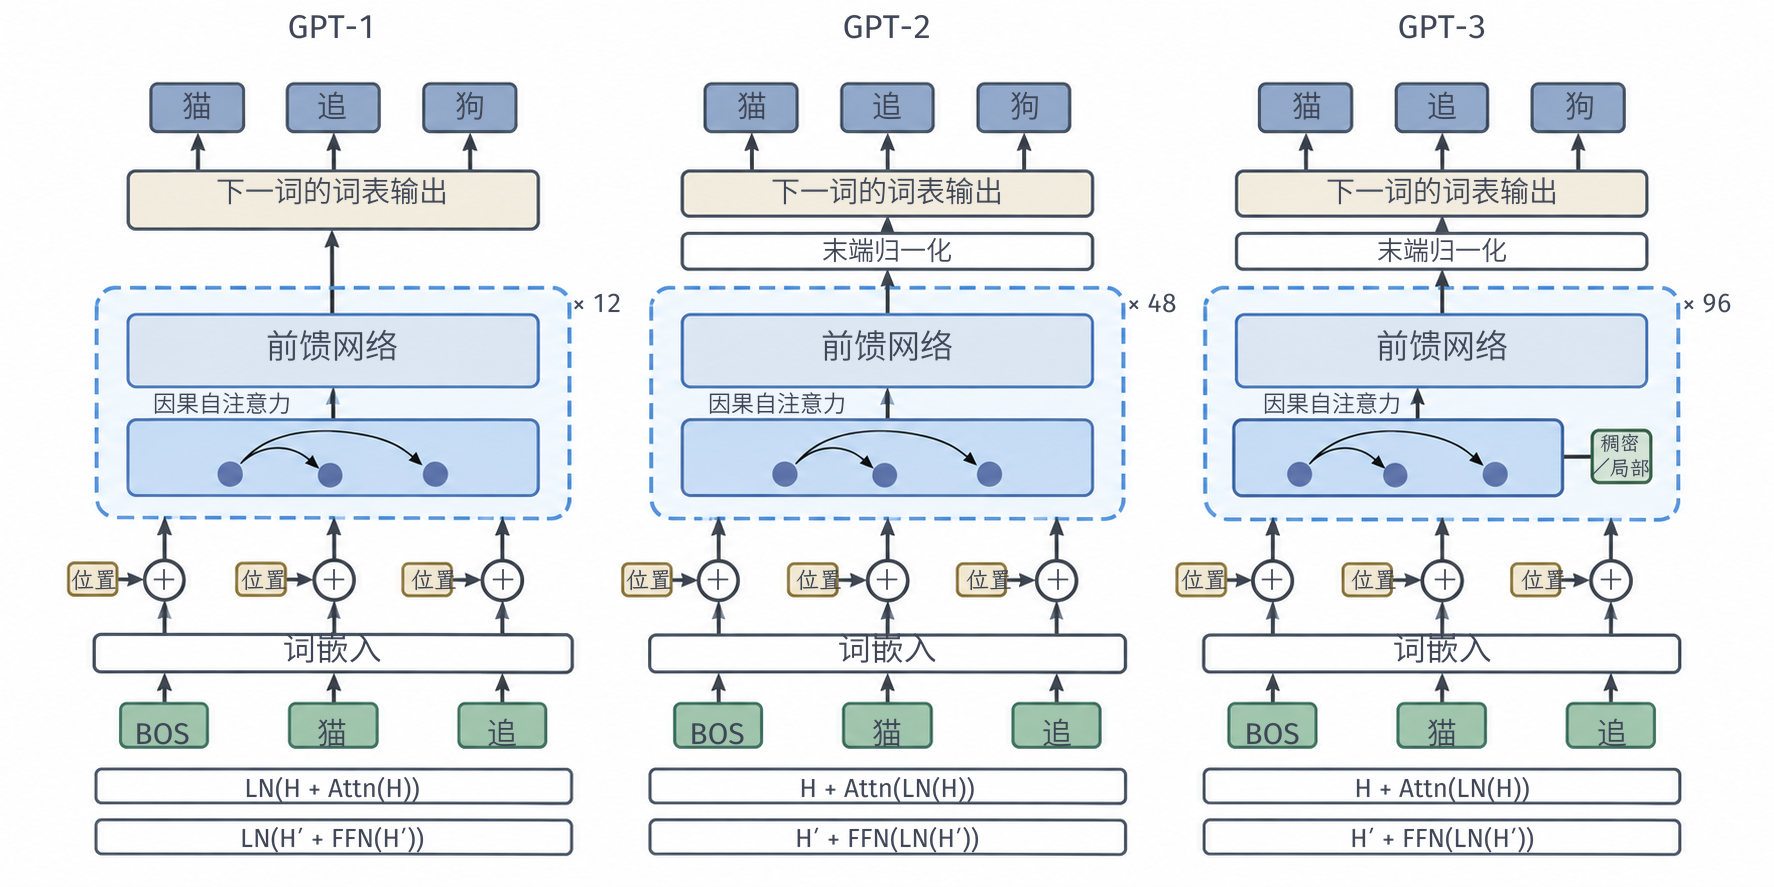
\includegraphics[width=150.199mm]{figures/05-neural-network-models/00-shared/generated/transformer-architecture-gpt/figure.png}
  \caption{GPT-1、GPT-2与GPT-3的公开块结构对比。各列下方的公式包括子层变换、残差和归一化；各版本中的$\operatorname{Attn}$均遵守因果约束。GPT-1采用Post-LN，GPT-2和GPT-3采用Pre-LN并增加堆叠末端归一化；GPT-3还交替使用稠密与局部带状注意力。层数指各原论文的最大公开配置，省略Dropout、内部投影和KV缓存；比较依据相应原论文。}
  \label{fig:transformer-architecture-gpt}
\end{figure*}

图中的竖直方向表示层数，水平方向表示词元位置。一次训练会让所有已知输入位置同时经过第1层，再同时经过第2层，依此向上；因果约束由每层的连接范围保证。生成时，前缀虽已知，尚未选出的下一词元却没有输入嵌入，因此不能提前计算它的各层表示。这就是“训练可以并行处理位置”和“生成仍逐词进行”能够同时成立的原因：两句话讨论的是不同阶段的已知输入。

同样以情感分类为例，GPT-1的预训练先学习文本接续，有监督微调再把句子末位置的表示接到分类头，并用类别标签更新模型。末位置可以因果读取整句，早期位置仍只能读取此前内容。原论文还在微调中保留辅助语言模型目标，让任务分类与文本预测共同参与参数更新；任务头与预训练词表头的预测对象不同。因而，“GPT是生成模型”描述了预训练与生成接口，并不意味着每个下游任务都必须把类别写成文本。

这条因果路径使训练目标与逐词生成直接对应，条件和输出可以采用统一的文本接口。早期位置的表示只使用当时前缀，BERT的词元表示则可结合后文；两类表示服务于不同可见条件。长输出还要依次建立新的前缀。用于分类时，因果模型可以在读完整段后的末位置作判断，也可以生成类别名称，但这与BERT在CLS上使用固定类别头的损失和输出空间不同。

\paragraph{GPT-2：调整归一化位置并扩大模型}

GPT-2保留因果解码器，将归一化从子层残差相加之后移到子层入口，形成Pre-LN，并在整个堆栈末端增加归一化。这样的变化修改了深层残差路径中的计算顺序，具体梯度差异可结合第\ref{sec:transformer-residual-normalization}节理解。GPT-2还扩大模型和网页训练语料，进一步考察不更新参数时的零样本迁移。原论文最大配置为48层、宽度1600、约15亿参数，上下文长度由GPT-1的512提高到1024\scite{radford2019gpt2}

在图中的块公式里，Post-LN和Pre-LN的差别落在残差路径上。Post-LN把原表示与子层增量相加后一起归一化；Pre-LN保留原表示，先把归一化后的副本交给注意力或FFN，再把所得增量加回来。因此，增加一层时，Pre-LN保留了一条直接传递原表示的路径。末端归一化则在整个堆叠完成后调整输出尺度。这里解释的是计算次序和梯度路径的变化，训练是否更稳仍受初始化、步长和模型深度影响。

GPT-2研究的零样本使用方式进一步改变了任务接口。比如把待概括的文章与一个摘要提示接成前缀，让词表头继续生成摘要文本，推理期间不为这篇文章更新模型参数。此时任务信息由输入文本提供，输出仍是下一词元分布。模型是否按所希望的格式作答，要在具体提示和数据上检验；能够把任务写成续写形式，只是给出了调用方法。

\paragraph{GPT-3：扩大规模并交替使用两种注意力连接}

GPT-3沿用GPT-2的总体组织与Pre-LN，但在不同层中交替采用稠密和局部带状稀疏注意力。前者允许当前位置读取全部已有前缀，后者只保留规定的局部连接；两者都遵守因果约束。最大的公开配置为96层、宽度12288、96个头、1750亿参数，上下文长度2048。论文系统研究了\term{上下文学习}，即把少量任务示例放入前缀，而不在该任务的推理阶段更新模型参数\scite{brown2020}

这一步同时涉及网络与使用方式：增加层数和宽度扩大了可学习参数，调整注意力连接改变了每层的信息路径，而在提示中提供示例改变的是当前输入。上下文学习通过当前提示提供任务信息，微调通过梯度改变模型参数；两者可以改变预测，却在不同对象上起作用。

为了看清上下文学习，可以构造一个情感判断提示：先给出“很好看：正面”和“太无聊：负面”，再放入“值得再看：”，让模型续写类别。两个带答案的例子都属于本次输入，最后的类别才是需要生成的输出。训练参数保持固定，注意力却会根据当前提示重新计算隐藏表示；换一组示例后，条件分布也可能改变。这与把同样两条标注样本用于梯度微调不同，后者会把变化保存在参数中。

把示例纳入前缀也有资源与统计上的限制。示例占用上下文位置，留给问题、文档和答案的空间会相应减少；排列次序、格式和标签表达还会改变实际输入。少样本提示是否降低任务错误，需要固定测试对象后比较，不能仅凭提示里出现了正确示例就保证新问题被正确回答。若提示中的例子包含了测试问题的答案，也不能把这次续写当作对未知答案的独立检验。

图中GPT-3的局部与稠密注意力则属于另一类改变。局部层只从规定范围读取，稠密层可以重新汇集整个允许前缀；较早的信息也可能已经被中间位置编码，再经后续层继续传递。因此，单个局部层的直接读取范围与整网能够建立的依赖范围不同。无论采用哪种连接，模型都须保持因果约束；上下文中的示例不会因此成为可以读取未来答案的通道。

\paragraph{InstructGPT与GPT-3.5阶段：让生成服从指令和对话}

续写目标奖励文本中的下一词元，人类指令任务还要求输出符合请求与偏好。InstructGPT在语言模型基础上加入人类示范的监督微调，再用人类偏好训练奖励模型并优化输出，使训练目标更贴近指令遵循\scite{ouyang2022instructgpt}2022年发布的ChatGPT则基于GPT-3.5系列模型进行了面向对话的微调。GPT-3.5是模型系列名称，ChatGPT是对话系统名称；这项演进说明基础训练之后的参数调整与对话交互；具体内部拓扑需要对应的架构材料才能确定\scite{openai2022chatgpt}

以“用两句话解释注意力”为输入，普通语言模型只按已有文本预测后续内容，可能生成回答，也可能接着续写另一条问题。监督微调用“指令—示范回答”明确希望它完成哪种接续；偏好训练再比较同一输入下的多个候选回答，使参数更新考虑人们更倾向于哪一种输出。基础生成路径仍逐词工作，改变的是训练所奖励的回答行为。奖励模型学到的是由标注形成的评价，不能因此把高奖励等同于事实正确。

进入多轮对话后，先前的用户输入和系统已经给出的回答也成为当前前缀的一部分。角色标记与消息边界帮助模型区分谁说了什么，因果计算则限定本次回答只能依据已提供的历史。若实现保存了历史键和值，可以复用相同前缀的计算；重新编辑历史、截去部分消息或改变输入格式后，缓存是否仍可用需要重新判断。对话形式改变了输入的组织，并不使已有模型参数在每轮交互中自动更新。

\paragraph{GPT-4与GPT-4o：扩展输入输出模态}

GPT-4的技术报告公开了图像与文本输入、文本输出，以及下一词元预训练和人类反馈后训练等信息，但明确未披露模型规模和详细内部架构。GPT-4o则进一步公开了文本、视觉与音频的端到端联合训练。这些公开材料支持比较模态、训练目标及接口能力；层数、专家数量与位置编码等内部细节则保留为未披露信息\scite{openai2023gpt4,openai2024gpt4o}

从本章已经建立的输入—网络—输出关系看，模态扩展至少带来两个需要分别说明的接口。图像或音频首先要形成网络能够处理的表示，并保留任务需要的空间、时间关系；输出端再把隐藏表示变成文本或其他模态的结果。仅知道某个系统能接收图像，无法确定它内部采用哪一种视觉前端，也无法确定视觉表示在多少层参与交互。因此，图中能够确认的输入输出按公开材料标明，未知的内部模块保持未展开。

\paragraph{GPT-5发布系统：在模型之间选择计算路径}

2025年GPT-5发布时，官方将其在ChatGPT中的形态描述为一个统一系统：路由器在快速响应模型与更深入的推理模型之间选择。这里的路由器选择的是整个模型；后文的混合专家模型（MoE）则在一个网络层内，为各词元选择少量计算分支。系统路由选择整条模型路径，层内路由选择词元计算分支；发布说明只支持前一种组织的描述，各模型的内部配置仍需单独披露\scite{openai2025gpt5}

图~\ref{fig:transformer-gpt-public-interfaces}进一步比较后续版本公开的接口和系统层次。灰色模块表示内部结构未完整披露；GPT-5发布系统的两条模型路径是系统级选择，它展示发布系统的选择流程，每个内部模型的专家组织留待相应资料说明。

\begin{figure*}[htbp]
  \centering
  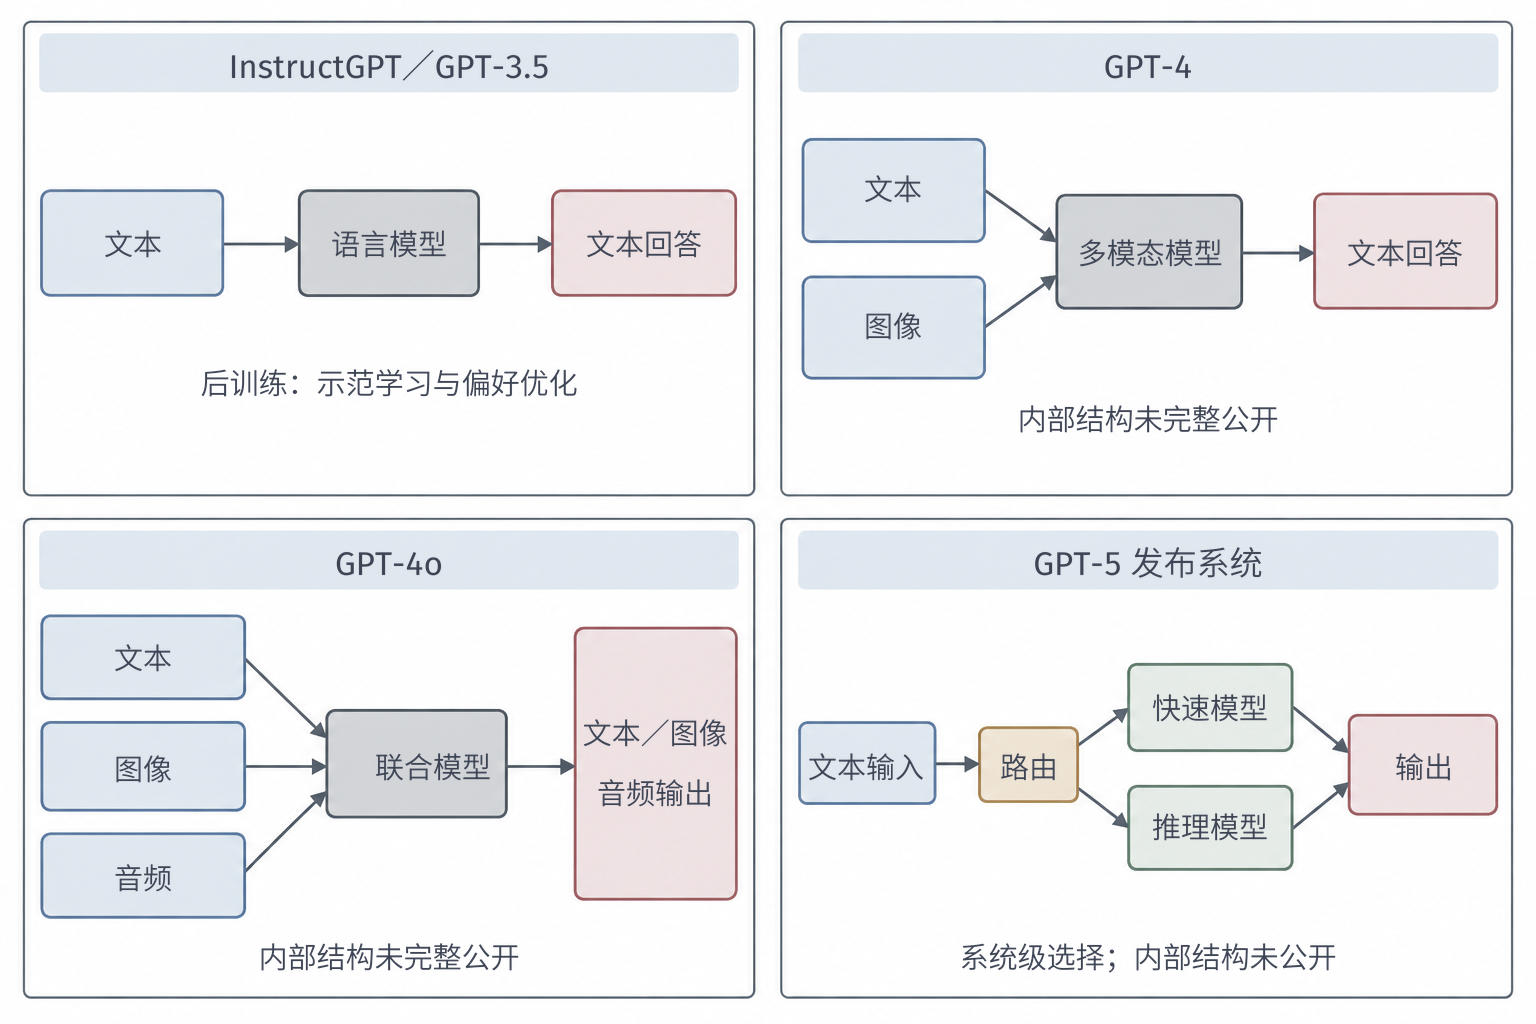
\includegraphics[width=130.048mm]{figures/05-neural-network-models/00-shared/generated/transformer-gpt-public-interfaces/figure.png}
  \caption{GPT后续代表版本的公开接口与系统组织。InstructGPT／GPT-3.5阶段主要改变后训练和交互；GPT-4支持图像与文本输入、文本输出；GPT-4o以文本、视觉、音频端到端联合训练，图示对应模型能力，特定产品功能以各发布阶段的实际开放范围为准；GPT-5发布系统在快速与深入推理模型间路由。灰色模块标明尚未披露的逐层细节，绿色模块仅标示所公开的计算路径。信息依据对应官方报告与发布说明，版本比较截至图中标注的发布阶段。}
  \label{fig:transformer-gpt-public-interfaces}
\end{figure*}

表~\ref{tab:transformer-gpt-generations}将各代变化对应到已经披露的对象。GPT-1至GPT-3可以比较具体块结构与配置；后续公开材料更多描述后训练、模态和系统组织，能够支持的比较也相应有所不同。

\begin{table*}[htbp]
  \centering
  \small
  \begin{tabular}{@{}p{25mm}p{64mm}p{66mm}@{}}
    \toprule
    代表版本 & 已公开的主要变化 & 阅读这些变化时应保留的区别 \\
    \midrule
    GPT-1（2018） & 因果解码器、Post-LN；12层、宽768；语言模型预训练后进行任务微调 & 预训练目标与下游任务监督可以不同 \\
    GPT-2（2019） & 改用Pre-LN并增加末端归一化；最大约15亿参数；1024词元上下文 & 零样本任务提示不需要再训练一个专用输出头 \\
    GPT-3（2020） & 延续Pre-LN；稠密与局部稀疏注意力交替；最大1750亿参数；2048词元上下文 & 提示中的少样本示例不等于梯度微调 \\
    InstructGPT／GPT-3.5阶段（2022） & 人类示范与偏好用于后训练；ChatGPT采用对话交互 & 基座模型、后训练方法和对话产品分属不同层面 \\
    GPT-4（2023） & 图像与文本输入，生成文本；内部架构细节未公开 & 多模态能力不提供确定参数量或专家数的证据 \\
    GPT-4o（2024） & 文本、视觉、音频端到端联合训练 & 模态扩展不能直接还原为一张已知的逐层网络图 \\
    GPT-5发布系统（2025） & 在快速响应与深入推理模型之间路由 & 系统级模型选择不等于层内词元级MoE \\
    \bottomrule
  \end{tabular}
  \caption{GPT家族的代表性演进。参数与上下文数字指相应原论文的配置，GPT-4之后列出官方明确披露的能力或系统组织，不推测未公开的网络细节；表格也不用于比较当前产品的可用性。}
  \label{tab:transformer-gpt-generations}
\end{table*}

\subsubsection{T5：把不同任务组织成文本到文本}

翻译生成另一种语言，分类输出一个类别，摘要输出较短文本；这些任务可以共享“读入条件文本、生成目标文本”的接口。\term{T5}（Text-to-Text Transfer Transformer）使用编码器—解码器，把任务说明和输入交给双向编码器，由因果解码器生成答案并交叉读取条件。它保留原始Transformer的两条路径，但采用相对位置偏置、Pre-LN和简化的归一化；原始基础FFN使用ReLU\scite{raffel2020t5}

T5的代表预训练任务是恢复被删去的连续片段。图~\ref{fig:transformer-architecture-t5}把“猫追狗”变成“猫$\langle S_1\rangle$狗”，解码器生成“$\langle S_1\rangle$追$\langle S_2\rangle$”，并以EOS结束生成。这些专用标记称为\term{哨兵词元}（sentinel token），作用是标明缺失片段及其边界。一个标记可以代替多个连续词元，因此目标长度可以变化。BERT在选中的输入位置恢复词元，T5在目标端串联缺失片段，逐步生成整段恢复内容。

\begin{figure*}[htbp]
  \centering
  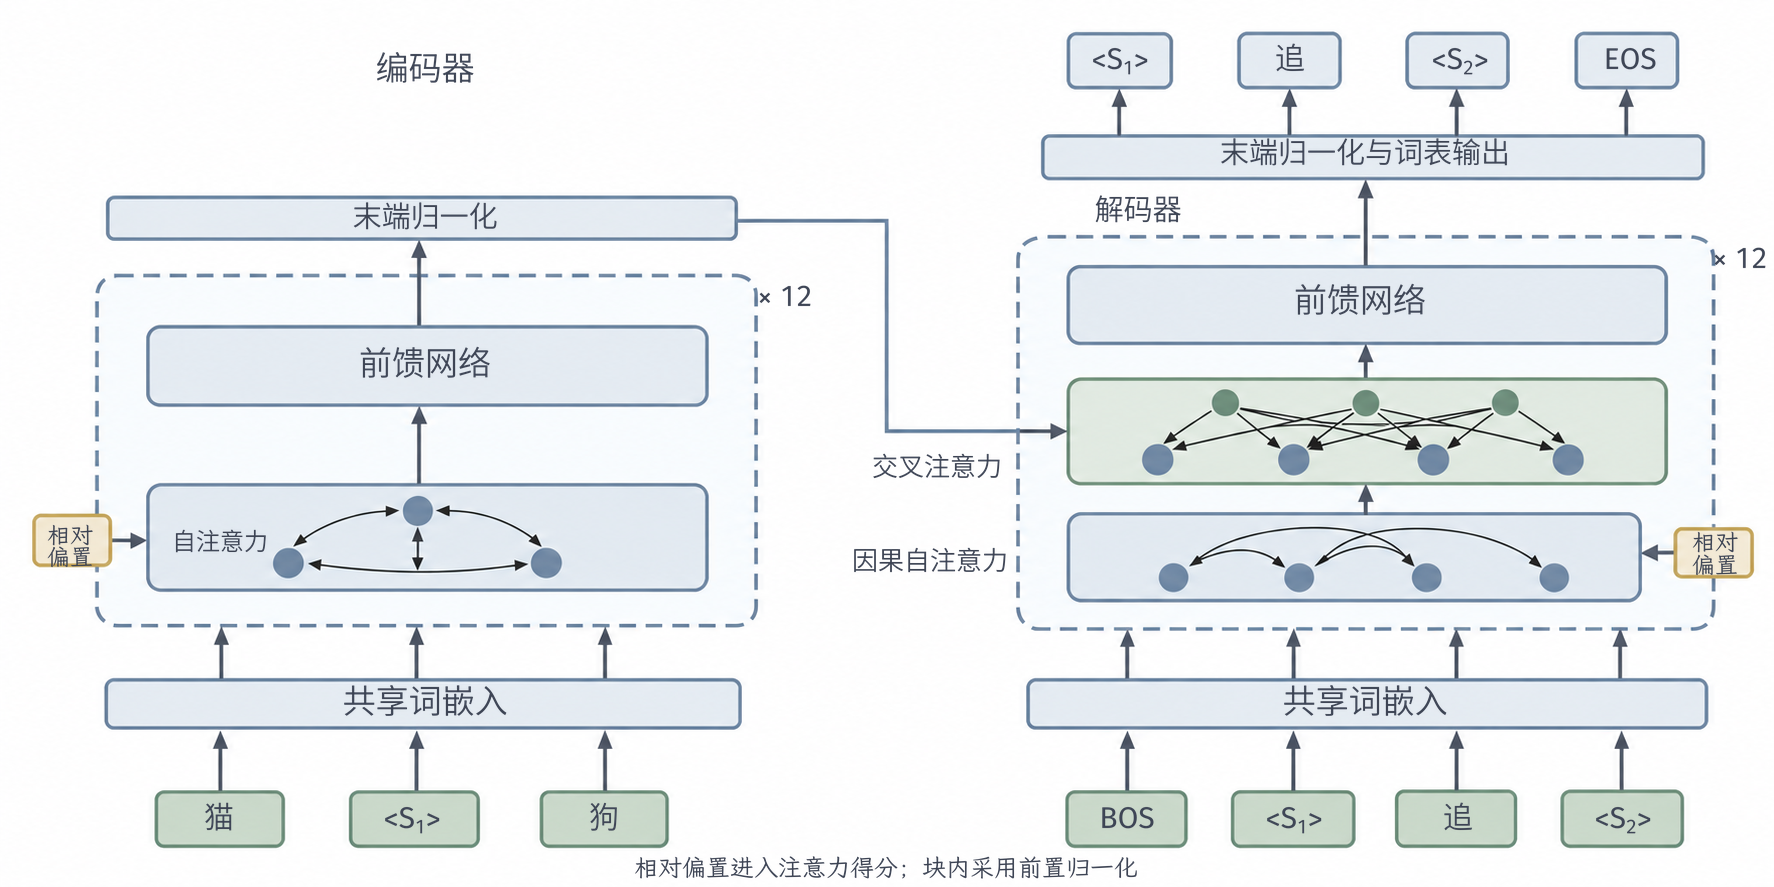
\includegraphics[width=150.199mm]{figures/05-neural-network-models/00-shared/generated/transformer-architecture-t5/figure.png}
  \caption{T5 Base的片段恢复与整网结构。$\langle S_1\rangle$替代源句中的缺失片段，目标中的同名标记引出恢复内容，$\langle S_2\rangle$结束该恢复片段，EOS结束生成。BOS表示解码起始输入。编码器与解码器各堆叠12个块，最终源表示供交叉注意力读取。相对位置偏置加入注意力得分，输入不叠加绝对位置向量。图中显式保留堆叠末端归一化，目标端与词表头合并展示；省略块内入口归一化、残差与Dropout。结构和任务依据Raffel等（2020）。}
  \label{fig:transformer-architecture-t5}
\end{figure*}

恢复目标由被删片段及哨兵标记串联而成，保留的源词元作为条件供解码器读取。给定扰动源句，按式\eqref{eq:transformer-conditional-loss}对恢复序列逐词计算损失；教师强制与因果掩码仍然适用。多处缺失按各哨兵的顺序组织，源长、缺失片段总长和标记数共同决定计算量。其Pre-LN仅按均方根调整尺度，保留可学习缩放，省去均值减除和平移项；本章标准LayerNorm另有这两项操作。

多个缺失片段更能说明哨兵的作用。假设把教学句“猫在院里追狗”中的“在院里”和“狗”分别删去，源端便是“猫$\langle S_1\rangle$追$\langle S_2\rangle$”，目标依次生成“$\langle S_1\rangle$在院里$\langle S_2\rangle$狗$\langle S_3\rangle$”，再输出EOS。源、目标中相同的标记指向同一缺口，最后一个新标记表示已没有后续待恢复片段。解码器只需生成被删内容及边界标记，保留下来的“猫”和“追”继续作为条件参与交叉读取。

这种接口使分类也能写成生成类别文本，任务之间不必各自规定一种输出头；源端双向理解与目标端因果生成的职责保持清楚。相应代价是仍要维护编码器、解码器与交叉注意力，生成式分类还需要规定合法类别词及其读出方式。任务可以复用文本输入输出的训练流程，所需目标长度、合法答案集合和评价量仍由各任务规定。



\subsubsection{架构之间如何取舍}

表~\ref{tab:transformer-common-architectures}将比较标准固定为已知条件、输出过程与结构代价。对一个具体任务，先判断后文何时可见、结果是否需要逐步生成，再选择网络组织。BERT与RoBERTa的主要差异位于预训练方案；原始Transformer与T5共享编码器—解码器组织，却采用不同的位置表示、归一化和任务目标。模型名称还包含训练方案与配置，信息流类型则按允许读取的来源与次序比较。

\begin{table*}[htbp]
  \centering
  \small
  \begin{tabular}{@{}p{24mm}p{34mm}p{47mm}p{50mm}@{}}
    \toprule
    代表模型 & 条件与读取规则 & 结构带来的便利 & 相应代价或使用边界 \\
    \midrule
    原始Transformer & 源双向；目标因果并交叉读取源 & 完整编码源句，生成时复用源表示 & 两组网络和交叉注意力；目标仍逐步产生 \\
    BERT & 扰动输入内双向读取 & 一次形成利用左右语境的各位置表示 & MLM不直接定义自由续写；任务需要适配输出头 \\
    RoBERTa & 与BERT同属双向编码 & 保持结构，改进预训练数据与优化方案 & 预训练投入增大；生成边界与BERT相似 \\
    GPT & 单一路径因果读取 & 前缀与答案共享接口，直接学习逐词生成 & 早期位置不读后文；长输出需要多步解码 \\
    T5 & 条件双向；目标因果并交叉读取条件 & 文本到文本接口统一多种任务 & 双堆栈成本；类别文本等仍需规定读出规则 \\
    \bottomrule
  \end{tabular}
  \caption{代表架构的优势与边界。比较的是信息流和任务接口，不是在不同参数量、训练数据与硬件下比较实测速度或任务分数。同一家族的后续版本还可能修改位置编码、归一化和前馈层。}
  \label{tab:transformer-common-architectures}
\end{table*}

架构规定了可计算的信息路径，训练数据决定模型见过什么，学习目标决定哪些行为受到奖励，解码与系统组织决定模型怎样被调用。这些因素共同构成实际预测过程，各项差异按输入、参数更新和执行步骤分别解释。


\FloatBarrier
\section{参数学习}
\label{sec:transformer-learning}

嵌入、注意力投影、前馈层、归一化和输出层由同一预测目标联合学习。一个批次中的样本可以具有不同有效长度，损失只覆盖监督位置；按样本平均与按词元平均会给予长序列不同权重，相应权重规定了经验目标与后续风险分析中的样本贡献。

在读具体推导前，先明确本节要回答的两个实践问题。第一，训练开始前这些参数应该取多大？Transformer里有多条对尺度特别敏感的路径——内容与位置相加的输入、点积得分、残差流上的逐次累加——初始化若不控制好，第一步的Softmax就可能饱和或让激活爆炸，因此初始化比普通前馈网络更讲究。第二，损失的梯度如何沿注意力这种新运算传回？这里有一条前馈网络里没有的分叉：注意力参数既改变“读出的值内容”，又改变“各位置的读取权重”，反向传播时这两条路径要分别计算后再汇合。本节先讨论初始化，再系统推导注意力与层归一化的导数；优化器、学习率调度及通用正则化由训练与泛化章节展开。

\subsection{参数初始化}
\label{sec:transformer-initialization}

为什么不能沿用单一的初始化方案？因为Transformer里不同参数所处的计算路径，其输出尺度对参数尺度的依赖方式不同，需要分别控制。第\ref{sec:ffn-initialization}节的对称性打破和方差传播原则仍然适用，但Transformer还需同时控制内容嵌入、点积得分与残差流的尺度。输入嵌入可从零均值分布初始化，不同词元独立采样；如果内容项使用$\sqrt d$缩放，初始方差应连同这一缩放考虑。可学习位置表也需要适当尺度，避免输入在尚未学习时被位置项完全主导。连续输入则应先明确量纲和训练数据归一化，再设置投影。

对不带激活的投影$\bm Y=\bm X\bm W$，若输入坐标零均值、方差为$s_x^2$，各权重彼此独立、与输入独立、零均值且方差为$s_w^2$，输入宽度为$d_{\mathrm{in}}$，简化计算给出输出坐标方差$d_{\mathrm{in}}s_w^2s_x^2$。可用Glorot尺度兼顾输入输出宽度，或用与$d_{\mathrm{in}}^{-1}$同阶的方差控制前向尺度；ReLU前馈支路则可采用式\eqref{eq:ffn-he-initialization}的思路。激活、门控和残差参数化会继续改变尺度，投影方差因此按各支路的输入与输出配置。

查询与键的初始尺度直接影响Softmax。若二者每坐标方差分别为$s_q^2,s_k^2$，沿用坐标独立和零均值近似，缩放后点积方差为$s_q^2s_k^2$。因此，除以$\sqrt{d_k}$只抵消宽度因素；过大的投影范数仍会使得分过尖。值与输出投影则决定注意力支路加入残差的大小。FFN的第二次投影也位于残差支路末端，应与第一投影和非线性一起检查输出尺度。

深度增加时，多次相加可能持续放大残差流。若一个简化子层写为$\bm h^{(l)}=\bm h^{(l-1)}+a_l\bm f^{(l)}$，且各增量与已有表示不相关、各坐标方差为$s_f^2$，则增量方差之和为$\sum_l a_l^2s_f^2$。取$a_l$与$L^{-1/2}$同阶可在这个近似下控制累积量；实际分支往往相关，深层训练还需联合考察这些相关性、梯度和归一化位置。缩小支路末端权重、显式残差缩放与可学习门控是不同参数化，后文会比较它们怎样控制新增支路。

归一化的缩放和平移常分别初始化为1和0；输出层按其输入宽度设置尺度。若输入输出共享嵌入，两处梯度会累积到同一参数，初始化也只执行一次。把整个投影都置零可能阻断上游学习：例如$\bm Q=\bm K=\bm0$时，得分对查询和键的局部梯度都为零。特定设计也会把少量支路末端置零。此时可沿计算图确定初始哪些参数有非零导数，以及后续更新怎样打开这些路径。

\subsection{反向传播}
\label{sec:transformer-backpropagation}

注意力的参数既影响“读取什么”，也影响“怎样评分”。理解这一点，就抓住了本节推导的主线：当输出出错时，误差既可以通过“被读出的值”往回传（这个值贡献得多，就该多改它），也可以通过“读取权重”往回传（这个位置读多了，就该调低它的得分）。两条路径在注意力处交汇，必须分别求清。为把两条路径分清，采用矩阵梯度记号$\bm G_{\mathrm X}=\partial\ell/\partial\bm X$，其形状与$\bm X$相同，并以Frobenius内积定义微分$\mathrm d\ell=\langle\bm G_{\mathrm X},\mathrm d\bm X\rangle_{\mathrm F}$。从式\eqref{eq:transformer-attention}中单头的$\bm Z=\bm A\bm V$开始，若下游给出$\bm G_{\mathrm Z}$，则
\begin{equation}
  \bm G_{\mathrm V}=\bm A^{\top}\bm G_{\mathrm Z},\qquad
  \bm G_{\mathrm A}=\bm G_{\mathrm Z}\bm V^{\top}\text{。}
  \label{eq:transformer-aggregation-gradient}
\end{equation}
值梯度汇集所有查询对同一值的读取贡献；权重梯度比较不同值对当前输出变化的作用。固定权重时仍有值梯度；学习读取比例时，还要从权重沿Softmax和评分继续回传。

对第$i$行，把有效权重写为列向量$\bm a_i$。Softmax各权重由共同分母耦合，将其Jacobian与该行权重梯度相乘，得到
\begin{equation}
  (\bm G_{\mathrm S})_{i,j}
   =\bm A_{i,j}\left((\bm G_{\mathrm A})_{i,j}
       -\sum_{t=1}^{n_s}\bm A_{i,t}(\bm G_{\mathrm A})_{i,t}\right)\text{。}
  \label{eq:transformer-softmax-gradient}
\end{equation}
这一求导将本章式\eqref{eq:transformer-softmax-scale-gradient}的局部Jacobian与上游梯度相乘。计算限定在有效集合上，被禁止的权重与得分梯度取零，以避免把无穷掩码当作普通浮点变量求导。每行得分梯度之和为零，与Softmax对整行得分加同一常数不变的性质对应。Softmax的共同分母让各权重相互影响：某个值的梯度要减去当前加权平均作用，才得到该位置的得分梯度。

\Needspace{45mm}
\begin{example}[从聚合误差到评分误差]
  \label{ex:transformer-gradient-numerical}
  沿用示例~\ref{ex:transformer-attention-numerical}未加掩码的情形，令$\ell=(\bm z_2)_2$，即只考察“追”的输出向量的第二坐标，上游梯度为$(0,1)^{\top}$。三个权重的梯度为$0,2,1$，加权平均为$5/4$，得分梯度因此为$-5/16,3/8,-1/16$，总和为零。值梯度则分别为$(0,1/4)^{\top}$、$(0,1/2)^{\top}$和$(0,1/4)^{\top}$。若最小化此目标，评分路径倾向于降低第二个值的权重，值路径还可以直接降低被读取的第二坐标；两种变化共同影响输出。
\end{example}

掩码固定时，对缩放点积继续求导可得
\begin{equation}
  \bm G_{\mathrm Q}=\frac{\bm G_{\mathrm S}\bm K}{\sqrt{d_k}},\qquad
  \bm G_{\mathrm K}=\frac{\bm G_{\mathrm S}^{\top}\bm Q}{\sqrt{d_k}}\text{。}
  \label{eq:transformer-qk-gradient}
\end{equation}
查询梯度聚合相关键，键梯度聚合读取它的查询；固定因果掩码只删除禁止的贡献。若得分还包含可学习位置偏置，相应参数按其使用的所有位置对累积得分梯度。

式\eqref{eq:transformer-qkv}的投影梯度为
\begin{equation}
  \begin{aligned}
    \nabla_{\bm W_{\mathrm q}}\ell&=\bm H_{\mathrm q}^{\top}\bm G_{\mathrm Q},\\
    \nabla_{\bm W_{\mathrm k}}\ell&=\bm H_{\mathrm s}^{\top}\bm G_{\mathrm K},\qquad
    \nabla_{\bm W_{\mathrm v}}\ell=\bm H_{\mathrm s}^{\top}\bm G_{\mathrm V},\\
    \bm G_{\mathrm H_{\mathrm q}}&=\bm G_{\mathrm Q}\bm W_{\mathrm q}^{\top},\\
    \bm G_{\mathrm H_{\mathrm s}}&=\bm G_{\mathrm K}\bm W_{\mathrm k}^{\top}
                      +\bm G_{\mathrm V}\bm W_{\mathrm v}^{\top}\text{。}
  \end{aligned}
  \label{eq:transformer-projection-gradient}
\end{equation}
交叉注意力的两侧接到不同上游模块；自注意力的两侧是同一矩阵，所以查询、键、值三条输入梯度需要相加。加入投影偏置时，其梯度为对应矩阵梯度沿位置求和。共享词元嵌入也按词元编号把各出现位置的贡献相加。

多头输出若为$\bm Y=\bm C\bm W_{\mathrm o}$，则$\nabla_{\bm W_{\mathrm o}}\ell=\bm C^{\top}\bm G_{\mathrm Y}$，$\bm G_{\mathrm C}=\bm G_{\mathrm Y}\bm W_{\mathrm o}^{\top}$。按拼接的列范围拆开$\bm G_{\mathrm C}$，各头分别执行上述求导，再将共同输入的梯度求和。各头分别更新自己的投影，共同输入则接收所有读取分支的梯度和。

残差相加把同一上游梯度送入直接路径和子层路径。对Pre-LN子层$\bm y=\bm x+F(\operatorname{LN}(\bm x))$，列向量记号下有
\begin{equation}
  \bm g_{\mathrm x}=\bm g_{\mathrm y}
     +\bm J_{\operatorname{LN}}^{\top}\bm J_F^{\top}\bm g_{\mathrm y}\text{。}
  \label{eq:transformer-preln-gradient}
\end{equation}
FFN沿用前馈求导。LN的每个输出坐标还依赖本行的均值与方差，输入梯度需要计入这些统计量随输入产生的变化。对式\eqref{eq:transformer-layernorm}的一行输入，先把中心化后的向量和公共分母分别记为
\[
  \bm c=\bm x-\mu\bm1,\qquad
  r=\sqrt{\frac1d\bm c^{\top}\bm c+\varepsilon}
   =\sqrt{s^2+\varepsilon}\text{，}
\]
其中$\mu=\mu(\bm x)$、$s^2=s^2(\bm x)$，且$\bm1^{\top}\bm c=0$、$r>0$。若归一化输出为$\bm y$，令$\widehat{\bm x}=(\bm x-\mu\bm1)/\sqrt{s^2+\varepsilon}=\bm c/r$、$\bm u=\bm g_{\mathrm y}\odot\bm\gamma$，以横线表示坐标平均。求输入梯度时固定$\bm\gamma$和$\bm\beta$，由$\bm y=\bm\gamma\odot\widehat{\bm x}+\bm\beta$可得$\mathrm d\ell=\bm u^{\top}\mathrm d\widehat{\bm x}$；因此$\bm u$就是反传到标准化向量$\widehat{\bm x}$的梯度。

先把$\bm c$视为输入，考察归一化分母的变化。由$r^2=d^{-1}\bm c^{\top}\bm c+\varepsilon$求微分，再对$\widehat{\bm x}=\bm c/r$使用乘积法则，得到
\[
  \mathrm d r=\frac{\bm c^{\top}\mathrm d\bm c}{d\,r},\qquad
  \mathrm d\widehat{\bm x}
    =\frac{\mathrm d\bm c}{r}
       -\frac{\bm c}{r^2}\,\mathrm d r\text{。}
\]
第一项是在分母暂不变化时，$\bm c$直接改变标准化向量的贡献；第二项计入所有坐标通过共同分母$r$产生的影响。把这两个微分代入$\mathrm d\ell$，并收集$\mathrm d\bm c$的系数，得到
\[
  \begin{aligned}
    \mathrm d\ell
      &=\frac{\bm u^{\top}\mathrm d\bm c}{r}
          -\frac{\bm u^{\top}\bm c}{r^2}\,\mathrm d r,\\
    \bm g_{\mathrm c}
      &=\frac{\bm u}{r}
          -\frac{\bm c\,(\bm c^{\top}\bm u)}{d\,r^3}\\
      &=\frac{\bm u-\widehat{\bm x}\,\overline{u\widehat x}}{r}\text{，}
  \end{aligned}
\]
其中$\bm g_{\mathrm c}=\partial\ell/\partial\bm c$，$\overline{u\widehat x}=d^{-1}\sum_{k=1}^d u_k\widehat x_k$是逐坐标乘积的平均。

再把$\bm g_{\mathrm c}$沿中心化运算传到$\bm x$。由于$\mu=d^{-1}\bm1^{\top}\bm x$，均值的变化会从每个坐标中一起减去，因而
\[
  \begin{aligned}
    \mathrm d\bm c
      &=\mathrm d\bm x-\frac1d\bm1\bm1^{\top}\mathrm d\bm x,\\
    \bm g_{\mathrm x}
      &=\bm g_{\mathrm c}-\overline{g_{\mathrm c}}\bm1\text{。}
  \end{aligned}
\]
这里$\overline{g_{\mathrm c}}=d^{-1}\sum_{k=1}^d(\bm g_{\mathrm c})_k$。中心化使$\overline{\widehat x}=0$，所以$\overline{g_{\mathrm c}}=\overline u/r$。代入前式并恢复$r=\sqrt{s^2+\varepsilon}$，得到
\begin{equation}
  \bm g_{\mathrm x}
   =\frac{\bm u-\overline u\bm1
             -\widehat{\bm x}\,\overline{u\widehat x}}
          {\sqrt{s^2+\varepsilon}}\text{。}
  \label{eq:transformer-layernorm-gradient}
\end{equation}
分子中的$-\overline u\bm1$来自减去行均值的反传，$-\widehat{\bm x}\,\overline{u\widehat x}$来自归一化分母随输入变化的反传。两项都在同一行内汇集坐标的作用，没有引入其他位置或样本的统计量；整个推导保留了$\varepsilon$，零方差输入的分母仍为正。
缩放和平移的梯度分别由$\bm g_{\mathrm y}\odot\widehat{\bm x}$和$\bm g_{\mathrm y}$沿位置、样本累积。训练中若使用Dropout，还需按前向使用的同一随机掩码回传。至此，输出损失可以经注意力的读取与评分、逐位置变换和残差路径，传到全部可训练参数；梯度提供参数更新方向，优化进展还取决于目标形状、步长及所用梯度估计。

\FloatBarrier
\section{Transformer的扩展}
\label{sec:transformer-extensions}

标准网络将输入表示、位置读取、特征变换和残差更新组合起来。此后大量研究都在回答同一个现实问题：当序列变得很长、模型变得很大时，标准Transformer的开销吃不消，应该在哪里动手？要在众多方法中不迷失，可以先区分它们改动的是三件不同的东西——读取规则本身（让谁和谁相连、用什么公式打分）、同一次计算的执行与存储方式（数学结果不变，只是算得更省）、以及每个位置内部的特征变换（注意力之外的FFN、归一化和连接）。扩展方法可以改变其中某个计算，也可以只改变同一计算的执行与存储方式。位置关系决定怎样匹配，特征选择决定哪些读取结果进入更新；位置对运算、中间激活及生成缓存又分别消耗计算和存储。扩展方法按这些具体目标调整不同部分。这些目标会影响不同资源，因而可以组合，也可能相互制约。下面依次考察位置编码、注意力、前馈层、归一化、深层连接和混合结构六类扩展，阅读时可不断追问：这个方法改变的到底是“算什么”还是“怎么算”，以及它省下的是计算、显存还是带宽。

\subsection{位置编码的扩展}
\label{sec:transformer-position-extensions}

顺序信息可以加到输入，也可以进入位置对评分。前者给每个位置一个表示，后者让读取直接依赖相对距离；旋转则提供了把位置变换嵌入点积的实现机制。下面固定内容投影，比较位置到底在哪里参与计算。

\subsubsection{绝对位置编码}

可学习位置表$\bm P\in\mathbb R^{n_{\max}\times d}$直接提供式\eqref{eq:transformer-input-position}中的$\bm p_i$，参数量为$n_{\max}d$。位置表只覆盖设定上限，扩充或插值提供新位置向量后，新增长度上的预测还需训练支持或相应外推检验。固定正弦编码对偶数宽度$d$定义
\begin{equation}
  \begin{aligned}
    (\bm p_i)_{2k+1}&=\sin(i\omega_k),\\
    (\bm p_i)_{2k+2}&=\cos(i\omega_k),\qquad
    \omega_k=10000^{-2k/d},
  \end{aligned}
  \label{eq:transformer-sinusoidal-position}
\end{equation}
其中$k=0,\ldots,d/2-1$，向量坐标从1开始，$i$采用本章从1开始的位置编号；改从0开始时需统一输入约定。不同频率使坐标随位置以不同速度变化，无需学习位置表，任意整数位置都可以求值。

图~\ref{fig:transformer-position-waves}把这个变化画成波形。为在同一位置区间内看清快慢，这里取$d=8$，只画$k=0,1$对应的前四个坐标：两对角频率分别为1和0.1弧度／位置。它与图~\ref{fig:transformer-position-example}的四维手算例采用相同公式，但宽度不同；四维例子的第二对频率是0.01，不能把两组参数混用。每对正弦与余弦具有相同周期，彼此相差四分之一周期；高频坐标随位置较快振荡，低频坐标变化较慢。同一横坐标处的各维幅值一起构成该位置向量，每条曲线只提供一个坐标。

\begin{figure}[t]
  \centering
  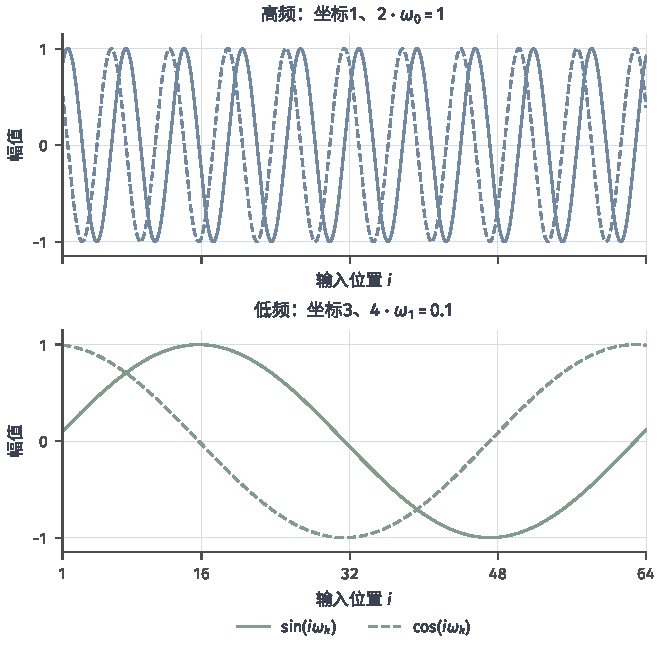
\includegraphics[width=105.412mm]{figures/05-neural-network-models/00-shared/matplotlib/transformer-position-waves/figure.pdf}
  \caption{固定正弦编码中选定坐标随输入位置的变化。取$d=8$，上图为坐标1、2（$k=0$），下图为坐标3、4（$k=1$）；两图横轴范围相同，幅值无量纲。实线为正弦，虚线为同频余弦，周期分别约为6.28和62.83个位置。连续曲线帮助观察波形，实际序列只在整数位置取值；本图仅示意选定维度，不是完整八维编码或训练结果。}
  \label{fig:transformer-position-waves}
\end{figure}

对固定距离$\Delta$，加法公式把$\bm p_{i+\Delta}$写为$\bm p_i$各坐标对的线性变换。这一变换给出位置位移的规律。完整注意力还处理内容投影，所以其得分可以同时依赖内容与位置。把内容和位置相加后，投影点积还包含内容与位置的交叉项；网络需要学习如何使用这些项。新位置向量可以直接求值；训练长度外的预测质量还取决于新上下文与距离如何进入已学计算。

\subsubsection{相对位置向量与距离偏置}

若任务更关心“相隔多远”而非“位于第几位”，绝对位置编码就显得不自然。语言里很多依赖只与相对距离有关（指代、搭配往往出现在邻近位置），与这句话在整篇文章中的绝对位置无关；整段话整体向后平移，词与词的关系应当不变，可每个词的绝对位置编号却全变了。可以直接让位置对得分依赖$j-i$，从而天然具有这种平移不变性。\term{相对位置编码}（relative positional encoding）为位置之间的关系提供表示。设$\bm r_{j-i}^{\mathrm k}\in\mathbb R^{d_k}$、$\bm r_{j-i}^{\mathrm v}\in\mathbb R^{d_v}$为距离对应的键和值修正，则一种形式为
\begin{equation}
  \begin{aligned}
    S_{i,j}&=\frac{\bm q_i^{\top}(\bm k_j+\bm r_{j-i}^{\mathrm k})}
                        {\sqrt{d_k}}+M_{i,j},\\
    \bm z_i&=\sum_j A_{i,j}(\bm v_j+\bm r_{j-i}^{\mathrm v})\text{。}
  \end{aligned}
  \label{eq:transformer-relative-position}
\end{equation}
这里$S_{i,j},M_{i,j},A_{i,j}$是对应矩阵元素的简写，$\bm q_i,\bm k_j,\bm v_j$是各行转置后的向量。键修正改变匹配，值修正把距离信息带入输出。Shaw等采用截断距离，共享过远位置的相对向量；这样限制参数数量，也合并了某些距离差异\scite{shaw2018relative}

若只需修改评分，可以使用标量偏置$b_{j-i}$，将其加到缩放点积上。偏置表可按距离截断或分桶，后者让一组距离共享参数；同一距离只存一个标量时，参数比同距离向量少；它调整评分，向量修正还可以改变匹配方向或输出内容。\term{线性偏置注意力}（attention with linear biases, ALiBi）在因果读取中采用
\begin{equation}
  S_{i,j}^{(a)}=\frac{\bm q_{i,a}^{\top}\bm k_{j,a}}{\sqrt{d_k}}
                 -m_a(i-j),\qquad j\leq i\text{，}
  \label{eq:transformer-alibi}
\end{equation}
其中$m_a>0$是第$a$头的预设斜率，未来位置仍由掩码排除。距离越远，扣除越多；不同斜率提供不同距离偏好。它无需训练长度对应的位置表，原论文在特定语言建模设置中检验了长度外推。这个结果依赖模型、数据与长度范围，线性距离偏好也可能不符合需要精确远距离访问的任务\scite{press2021alibi}

回到“猫／追／狗”，图~\ref{fig:transformer-position-extensions}把相对位置写成可逐格检查的距离矩阵。“追”读取“狗”对应$j-i=1$；若整段句子在更长文本中同时后移5位，距离仍为$8-7=1$。ALiBi进一步把距离变成得分修正：图中“狗”读取三个位置时分别扣除$1.0,0.5,0$，之后才做Softmax。图~\ref{fig:transformer-position-example}是在输入上相加，而这里是在每一对位置的评分上相加，两个操作作用于不同对象。

\begin{figure*}[htbp]
  \centering
  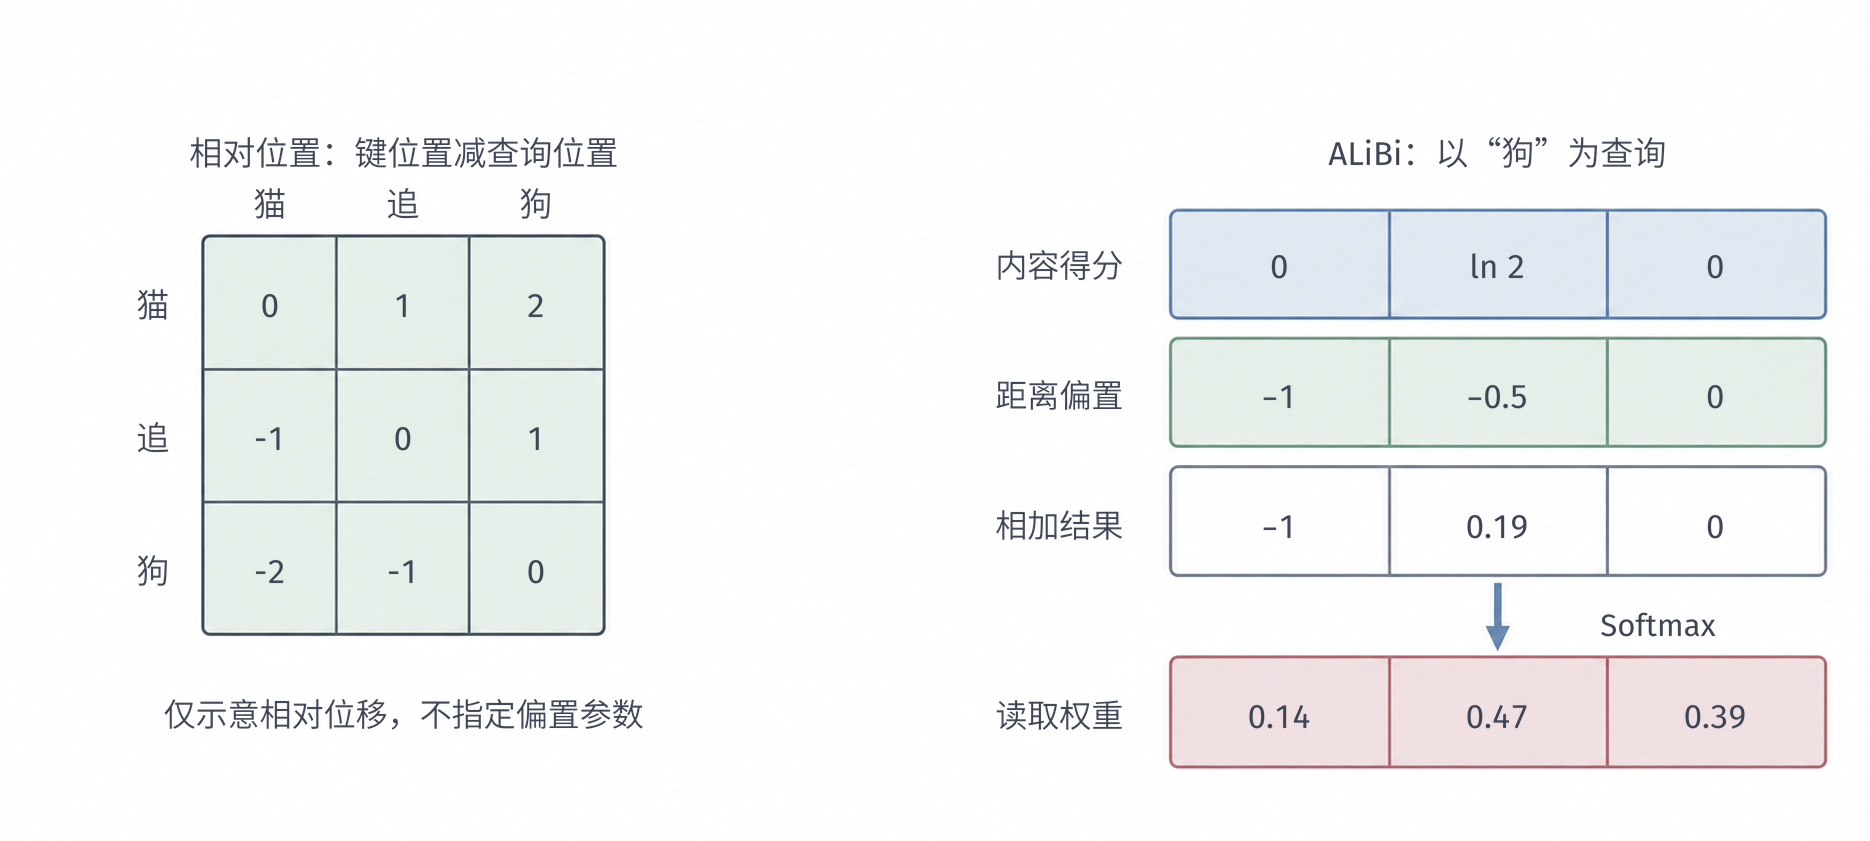
\includegraphics[width=158.327mm]{figures/05-neural-network-models/00-shared/generated/transformer-position-extensions/figure.png}
  \caption{“猫／追／狗”的相对位置。左图行是查询位置$i$、列是键位置$j$，格内为$j-i$，正负号区分左右方向。右图取“狗”为查询、斜率$m=0.5$，演示ALiBi如何修正教学得分并重新归一化；显示数值保留两位小数，真实计算使用未舍入值。}
  \label{fig:transformer-position-extensions}
\end{figure*}

\FloatBarrier
\subsubsection{旋转位置编码}

查询与键怎样变换，决定位置如何进入它们的点积。绝对向量相加会引入内容与位置的交叉项；另一种构造直接控制位置对关系：分别根据位置$i$、$j$变换查询和键，但要求变换后的点积只通过$j-i$依赖位置。\term{旋转位置编码}（rotary position embedding, RoPE）用旋转实现这一要求：位置决定旋转角度，两向量的相对角度进入点积\scite{su2021roformer}

\paragraph{为什么旋转能表示位移}
先考虑二维向量。希望位置每增加1，就施加同一个变换，而且连续移动$i$步再移动$j$步，应等价于移动$i+j$步。平面旋转满足这种组合规律，还能保留向量长度。设每步旋转$\omega$弧度；单位横轴旋转$\theta$后变为$(\cos\theta,\sin\theta)^{\top}$，单位纵轴变为$(-\sin\theta,\cos\theta)^{\top}$。把它们作为两列，就得到
\begin{equation}
  \bm R(\theta)=
  \begin{pmatrix}
    \cos\theta&-\sin\theta\\
    \sin\theta&\cos\theta
  \end{pmatrix}\text{。}
  \label{eq:transformer-rope-rotation}
\end{equation}
对尚未施加本层RoPE旋转的查询$\bm q_i=(q_{i,1},q_{i,2})^{\top}$，令
\[
  \widetilde{\bm q}_i=\bm R(i\omega)\bm q_i
  =\begin{pmatrix}
     q_{i,1}\cos(i\omega)-q_{i,2}\sin(i\omega)\\
     q_{i,1}\sin(i\omega)+q_{i,2}\cos(i\omega)
   \end{pmatrix}\text{；}
\]
键同样取$\widetilde{\bm k}_j=\bm R(j\omega)\bm k_j$。这里旋转的是投影后的查询和键，内容向量仍决定旋转前的方向和长度。

\paragraph{从两个绝对角度推到相对位置}
矩阵转置把旋转角取反。再利用三角函数的和角公式，逐项相乘可得
\begin{equation}
  \begin{aligned}
    \bm R(\alpha)^{\top}&=\bm R(-\alpha),\\
    \bm R(\alpha)\bm R(\beta)&=\bm R(\alpha+\beta),\\
    \bm R(i\omega)^{\top}\bm R(j\omega)
      &=\bm R((j-i)\omega)\text{。}
  \end{aligned}
  \label{eq:transformer-rope-composition}
\end{equation}
令$\Delta=j-i$，代入两向量的点积，有
\begin{equation}
  \begin{aligned}
    \widetilde{\bm q}_i^{\top}\widetilde{\bm k}_j
      &=\bm q_i^{\top}\bm R(\Delta\omega)\bm k_j\\
      &=(q_{i,1}k_{j,1}+q_{i,2}k_{j,2})\cos(\Delta\omega)\\
      &\quad +(q_{i,2}k_{j,1}-q_{i,1}k_{j,2})\sin(\Delta\omega)\text{。}
  \end{aligned}
  \label{eq:transformer-rope-two-dimensional}
\end{equation}
两个内容乘积组合分别乘上余弦和正弦，位置只以$\Delta$出现。若保持内容向量固定，把$i$和$j$同时加上$c$，差值不变，点积也不变。同时平移位置编号保持了这次位置变换；若上下文也改变，旋转前的查询与键会随网络计算改变，完整输出仍可能不同。

图~\ref{fig:transformer-rope}给出可手算的例子。取“追”的位置$i=2$、“狗”的位置$j=3$，并令$\bm q_i=\bm k_j=(1,0)^{\top}$、$\omega=\pi/6$。旋转后
\[
  \begin{aligned}
    \widetilde{\bm q}_i&=(1/2,\sqrt3/2)^{\top},\qquad
    \widetilde{\bm k}_j=(0,1)^{\top},\\
    \widetilde{\bm q}_i^{\top}\widetilde{\bm k}_j
      &=\sqrt3/2=\cos((3-2)\pi/6)\text{。}
  \end{aligned}
\]
两个向量分别转过$60^\circ$和$90^\circ$，点积由$30^\circ$的夹角决定。这里的频率为画图方便而选取；一般内容向量原本就有自己的夹角，旋转在其上叠加位置差带来的角度。

\paragraph{从二维构造完整注意力头}
若$d_k$为偶数，将坐标按$(1,2),(3,4),\ldots,(d_k-1,d_k)$两两配对。第$u$对使用频率$\omega_u=10000^{-2u/d_k}$，其中$u=0,\ldots,d_k/2-1$。把各旋转块放在对角线上，定义
\[
  \bm R_i=\operatorname{diag}\!\left(
    \bm R(i\omega_0),\ldots,\bm R(i\omega_{d_k/2-1})\right)\text{。}
\]
各对坐标独立旋转，完整点积就是它们各自点积之和，因此二维推导逐块成立：
\begin{equation}
  \begin{aligned}
    \widetilde{\bm q}_i&=\bm R_i\bm q_i,\qquad
    \widetilde{\bm k}_j=\bm R_j\bm k_j,\\
    \widetilde{\bm q}_i^{\top}\widetilde{\bm k}_j
      &=\bm q_i^{\top}\bm R_i^{\top}\bm R_j\bm k_j
       =\bm q_i^{\top}\bm R_{j-i}\bm k_j\text{。}
  \end{aligned}
  \label{eq:transformer-rope-relative}
\end{equation}
随后仍按式\eqref{eq:transformer-attention}除以$\sqrt{d_k}$、加掩码并做Softmax。由于$\bm R_i^{\top}\bm R_i=\bm I$，旋转保留查询和键的范数。实现只需逐坐标对计算正弦、余弦和乘加，不必构造稠密的$d_k\times d_k$矩阵；部分坐标也可以保留未旋转形式。这里按相邻坐标配对，其他配对实现则相应重排投影坐标与缓存，保持同一旋转约定。

\paragraph{生成时怎样复用旋转结果}
标准用法旋转查询与键，不旋转值。在后文介绍的KV缓存中，第$t$个位置到来时，只需计算$\widetilde{\bm q}_t=\bm R_t\bm q_t$和$\widetilde{\bm k}_t=\bm R_t\bm k_t$，将旋转后的键与原值$\bm v_t$追加保存。新查询与旧键$\widetilde{\bm k}_j$做点积，式\eqref{eq:transformer-rope-relative}自然给出相对位移$j-t$；已经旋转过的旧键无需再按当前步旋转。词元的逻辑编号决定旋转角度，缓存放在哪个物理地址只决定从哪里读出数值。这种复用要求位置编号、旋转频率与位置缩放规则保持一致；若改变这些规则，旧缓存也需要相应转换或重算。

各频率决定角度随位置改变的速度，单个坐标对的点积可以随距离振荡。例如前述单位向量的得分是$\cos(\Delta\omega)$，这个例子的各次振荡由所取频率决定。RoPE在新位置可以求值，预测仍可能遇到训练未覆盖的相位和距离分布；调整频率或位置尺度会改变读取规律，需要在预期长度范围重新检验。

\begin{figure}[htbp]
  \centering
  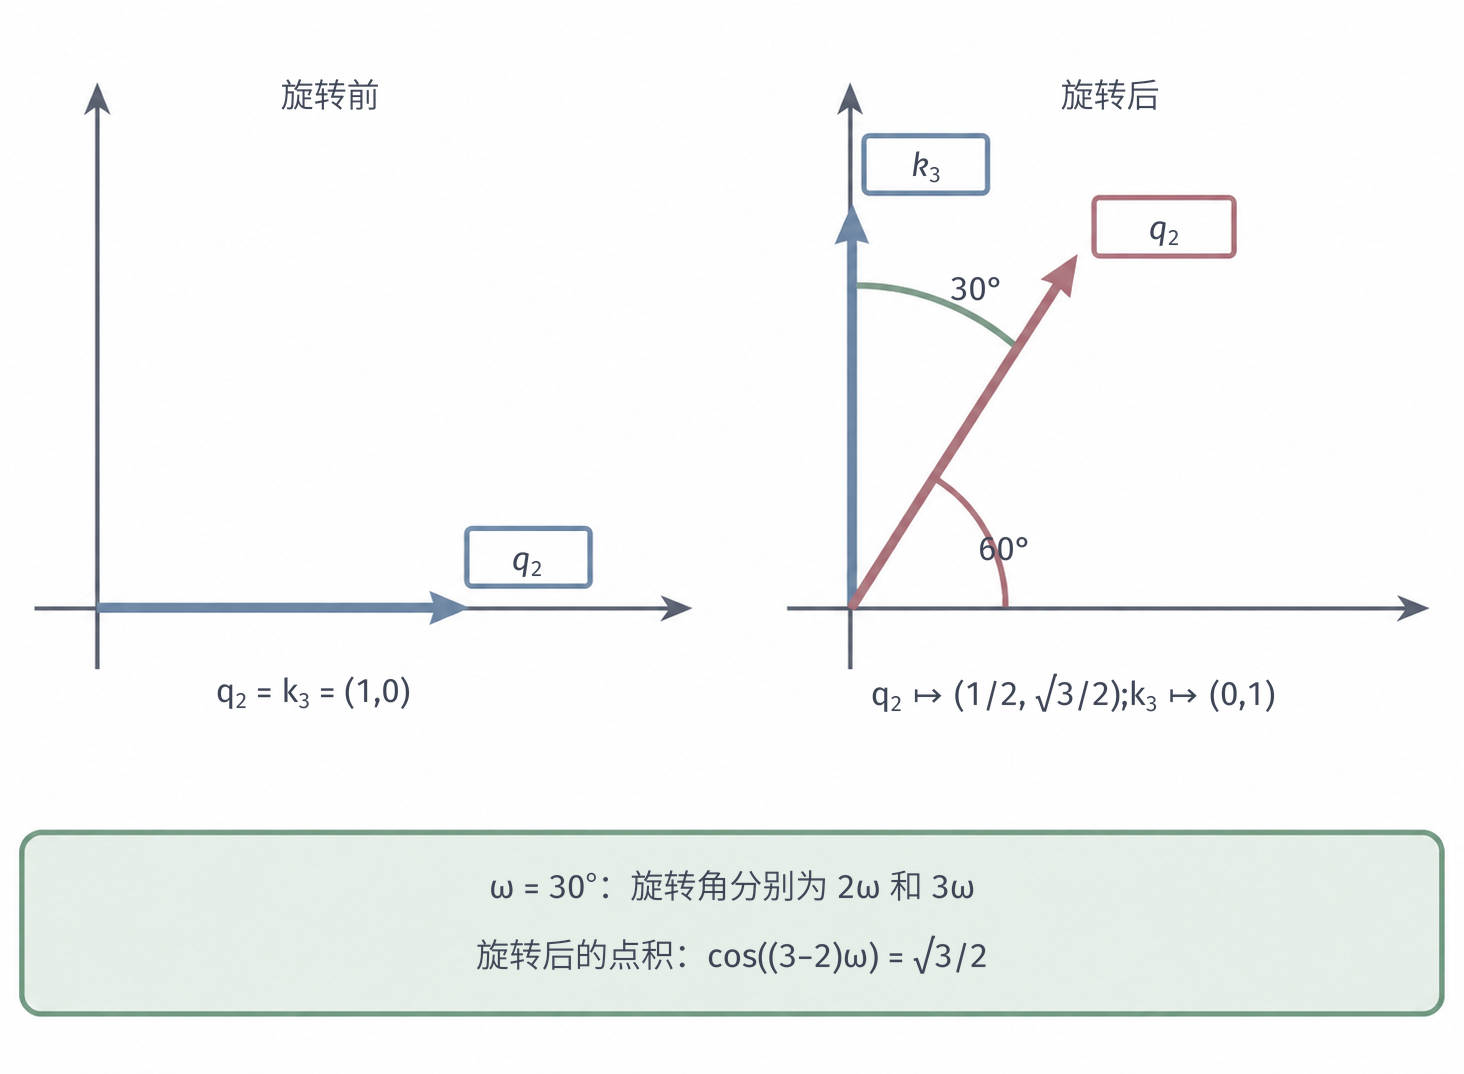
\includegraphics[width=112.000mm]{figures/05-neural-network-models/00-shared/generated/transformer-rope/figure.png}
  \caption{RoPE在一个二维坐标对中的作用。左图两个内容向量重合；右图“追”的查询和“狗”的键按各自位置旋转，夹角为$(3-2)\omega=30^\circ$，点积因此依赖相对位置。示例频率为$\pi/6$，用于演示几何关系；实际模型对多个坐标对采用不同频率，并保留各自的内容向量。}
  \label{fig:transformer-rope}
\end{figure}

绝对与相对描述的是位置关系，旋转描述的是注入机制，一个按绝对编号执行的旋转，可以在点积中形成相对距离关系。可学习绝对表有显式长度参数，固定正弦和RoPE无需位置表，距离偏置由距离覆盖或斜率决定参数量；位置计算的资源与覆盖范围可以据此比较，训练长度外的误差则还需要任务和数据条件。图像还需要保留二维位置，连续时间数据需要处理实际时间间隔，单一序列编号未必足够。



\subsection{注意力机制的扩展}
\label{sec:transformer-attention-extensions}

先看增量生成时一个朴素实现会浪费什么。逐词生成时，每产生一个新词，都要让它去读取此前所有位置；若每一步都把整个前缀重新跑一遍注意力，前面那些早已算过、且不会再变的键和值就被反复重算。\term{键值缓存}（key--value cache, KV cache）保存每层已有位置的键和值，生成时只计算新位置的投影并追加，避免这种重复。固定参数、位置编号和因果掩码时，旧位置表示不依赖未来输入，所以其键值可以复用；如果前缀内容或可见规则改变，原缓存未必继续有效。

对$L$层、$h$头、每头$d_k=d_v$、当前长度$n$的单序列，标准缓存有$2Lnhd_k$个元素，字节量还要乘以每元素的存储字节数和批量大小。旧位置的投影与网络块结果可直接复用，新查询则继续读取$n$个键和值，其位置对算术量为$O(nhd_k)$。将长度从1生成到$n$时，稠密注意力累计仍有平方量级的位置对读取。预填充（prefill）是一次处理已知前缀并建立缓存，逐步解码（decoding）则复用缓存产生后续内容；两者的并行规模和存储瓶颈不同。

\subsubsection{模型效果：信息范围与特征选择}

\paragraph{支持不同信息来源与可见范围}

交叉注意力改变键值来源，因果注意力改变允许的连接，两者可以同时出现于同一目标块。还有一种常见情形介于两者之间：条件生成时，已知的提示或源前缀可以放心地彼此双向读取（它是完整给定的），但正在生成的目标只能读此前内容、不能反向污染条件。\term{前缀注意力}（prefix attention）让给定条件前缀内部互相读取，而目标位置读取前缀和此前目标；前缀表示只由条件前缀形成；若加入目标信息，原来的前缀表示便会改变，需要重新编码。图~\ref{fig:transformer-masks}固定“猫／追／狗／EOS”四个位置，对比三种掩码。前缀方案把“猫追”设为已知条件，两位置内部可以互读；生成“狗”时可以读取这段条件，而“狗”的信息不能反向进入已缓存的条件表示。掩码将条件输入与生成前缀的可见范围直接写入每层计算。

\begin{figure*}[htbp]
  \centering
  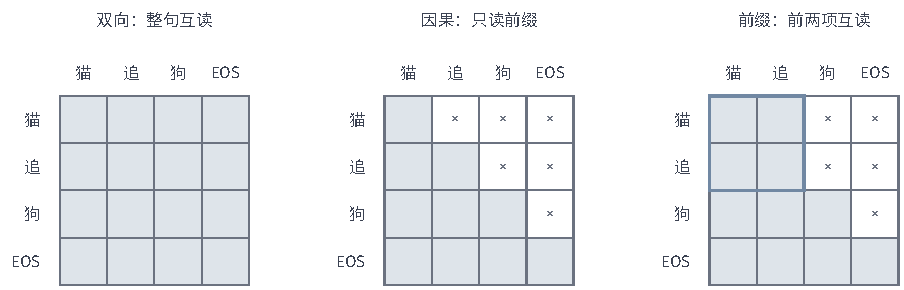
\includegraphics[width=153.003mm]{figures/05-neural-network-models/00-shared/tikz/transformer-masks/figure.pdf}
  \caption{四个位置的读取范围。行表示查询位置$i$，列表示键位置$j$，着色格允许读取，带叉白格禁止读取。左为全部有效输入间的双向读取，中为$j\leq i$的因果读取，右为前两个位置构成条件前缀的读取：前缀内部双向，目标读取全部前缀与截至当前位置的目标输入。目标输入已移位，因此读取当前输入不等于读取当前待预测标签。}
  \label{fig:transformer-masks}
\end{figure*}

\paragraph{优化动态信息选择：门控注意力}

Softmax每行必须把总权重1分配给可见值，即使这些值都不适合当前更新——它只能在候选之间做“相对取舍”，无法表达“这次谁都不值得读、干脆什么都不取”。要获得这种整体开关能力，需要在注意力之外再加一个不被归一化为1的控制量。\term{门控注意力}（gated attention）增加一个输入相关的控制量，调节特征或聚合结果的通过程度。例如，对第$a$头在位置$i$的结果，可以令
\begin{equation}
  \bm g_{i,a}=\sigma(\bm W_{\mathrm g,a}^{\top}\bm h_i+\bm b_{\mathrm g,a}),\qquad
  \widetilde{\bm z}_{i,a}=\bm g_{i,a}\odot\bm z_{i,a}\text{，}
  \label{eq:transformer-gated-attention}
\end{equation}
其中$\bm W_{\mathrm g,a}\in\mathbb R^{d\times d_v}$，Sigmoid门与头输出同宽。每头一个标量门则把整头共同缩放。注意力权重选择“从哪些位置读取”，输出门决定“这次读取的哪些特征应通过”，两者作用对象不同。

门也可置于值投影之后或最终输出投影之后，这些位置通常不等价。值门改变不同来源的内容，查询相关的输出门改变接收端结果。Qiu等比较了门的位置和粒度，并在所测试的大语言模型配置中观察到聚合后Sigmoid门对训练与表示行为的改善；观察到的改进对应论文中的训练配置，其作用范围由模型、目标及数据确定。逐坐标门增加非线性和参数，也要考虑饱和造成的梯度减弱\scite{qiu2025gated}

图~\ref{fig:transformer-gated-attention}接着使用“追”的聚合结果$(0.5,1.25)^{\top}$。若当前表示生成的门为$(0.2,0.8)^{\top}$，逐坐标相乘得到$(0.1,1.0)^{\top}$，分别保留第一维的20\%与第二维的80\%。位置权重在此前已经完成归一化，门按坐标调整混合后的特征，来源位置的权重仍由前面的Softmax给出。标准点积和键值存储都已在门控前完成，其成本继续保留。

\begin{figure*}[htbp]
  \centering
  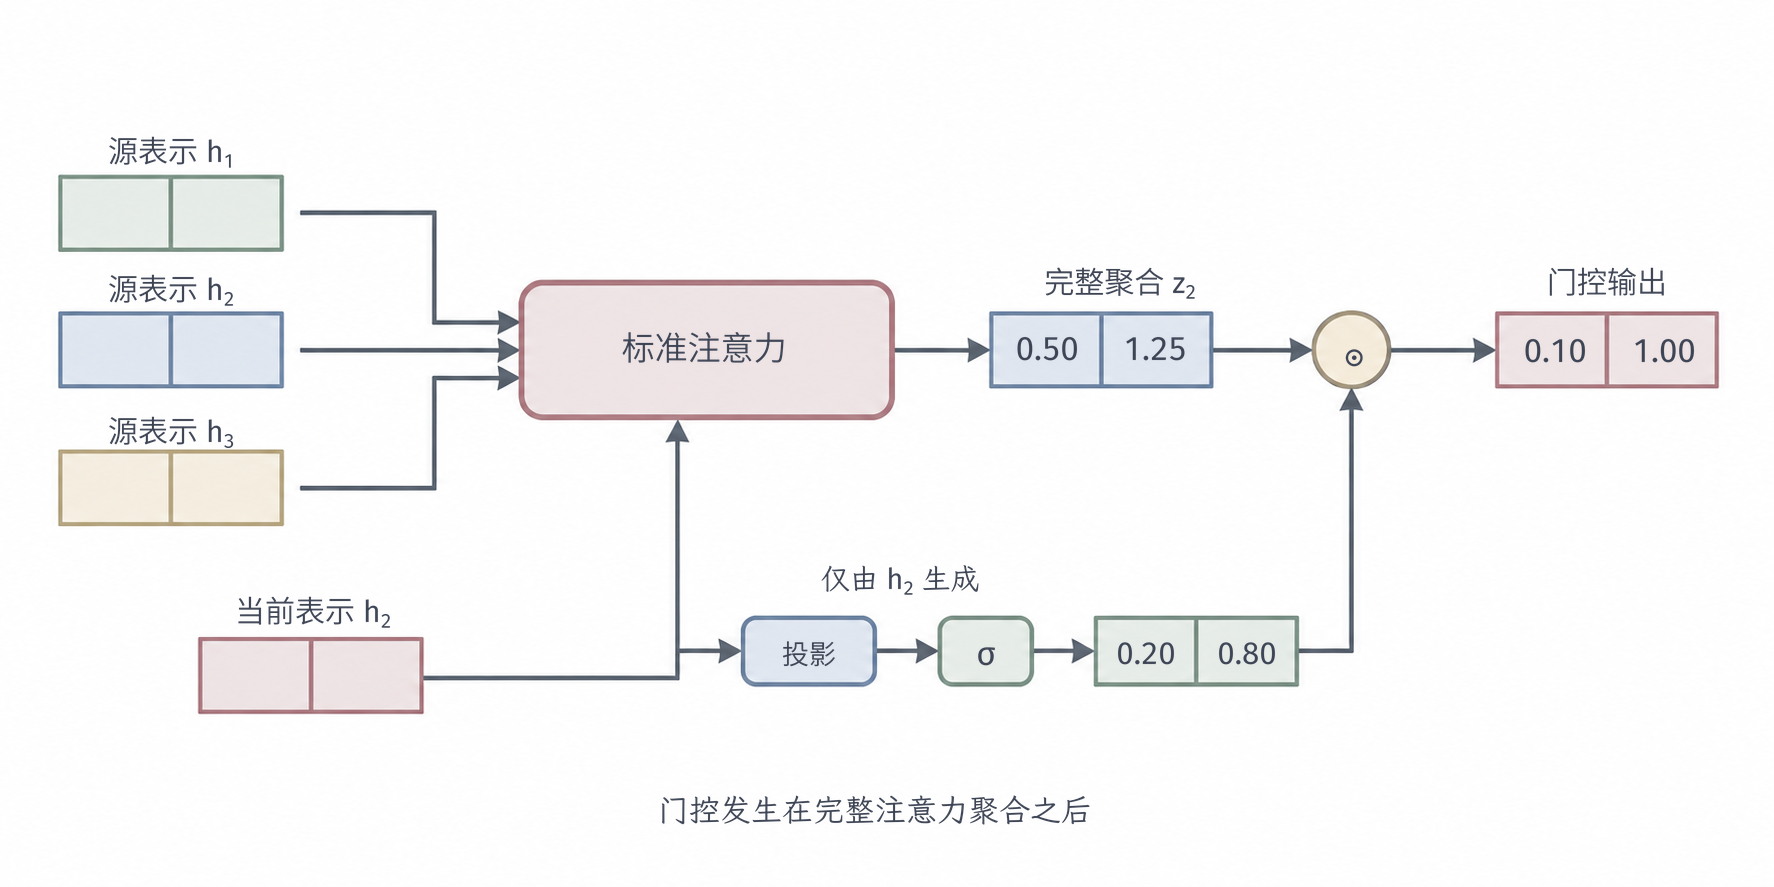
\includegraphics[width=150.199mm]{figures/05-neural-network-models/00-shared/generated/transformer-gated-attention/figure.png}
  \caption{以“追”为查询的聚合后门控。左支路从整段序列读取内容，右支路仅由当前词元表示产生Sigmoid门。教学数值中，聚合结果$(0.5,1.25)$与门$(0.2,0.8)$逐坐标相乘，得到$(0.1,1.0)$。门控制的是输出特征，而不是三个来源位置的概率；图中固定一个头并省略头索引、多头拼接和输出投影，数值并非训练测量。}
  \label{fig:transformer-gated-attention}
\end{figure*}

\subsubsection{训练效率：位置交互与中间存储}

整段训练需要为位置对评分，还要为反向保存或重算中间量。标准稠密注意力的开销主要压在两处：一是$n^2$量级的位置对算术，二是那个$n\times n$得分／权重矩阵带来的中间存储与显存搬运。针对它们，研究上形成了思路清晰的几条路线——直接删掉用不上的连接（稀疏）、换掉Softmax核从而改变求和次序（线性）、把$n$个位置压成少数几个汇总槽（低秩），以及数学结果不变、只优化存储搬运方式（FlashAttention）。连接数影响前一成本，聚合公式与执行方式影响后者及其访存；下面分别说明这些改动在训练和推理中的适用范围。

\paragraph{降低位置连接的计算量：稀疏注意力}

\term{稀疏注意力}（sparse attention）只计算保留的连接。它的依据是一个经验观察：对很多任务而言，真正有用的位置对并不是全部$n^2$个——一个词通常主要依赖邻近的词，再加上少数几个全局关键位置；既然如此，大量远距离连接的权重本来就接近零，为它们付出计算并不划算。例如每个位置读取$w$个窗口位置，再加少量全局位置，若各头保留连接总数为$e_{\mathrm{att}}$，评分和聚合需要$O(e_{\mathrm{att}}(d_k+d_v))$算术操作，权重存储为$O(e_{\mathrm{att}})$。窗口大小和全局连接数固定时，连接数随$n$线性增长；窗口若随$n$增长，复杂度也相应保留窗口长度因子。Sparse Transformer采用特定稀疏分解，使连接数达到$O(n\sqrt n)$量级，其稀疏连接仍多于固定窗口的线性规模$O(n)$\scite{child2019sparse}

删除连接也改变传播范围。只有窗口连接时，一层无法读取窗口之外的信息，跨层传播可扩大范围，却增加依赖路径长度；全局位置使远处信息有较短通路，但也可能形成汇总瓶颈。保留哪些连接决定哪些证据能够到达目标位置，相同比例的稀疏模式也可能形成不同通路。

\paragraph{降低聚合计算量：线性注意力}

\term{线性注意力}（linear attention）把位置对核改写为有限维特征内积，以改变聚合次序。它的关键想法是一条代数恒等式带来的计算次序重排：标准注意力必须先算好每一对（查询，键）的权重，再对值求和，因而绕不开$n^2$个位置对；若相似度能写成“查询特征”和“键特征”的内积，就可以利用结合律先把所有键和值汇总成一份与查询无关的状态，再让每个查询去读这份状态，从而把成本降到对$n$线性。它仍按归一化的成对相似度读取值，但将相似度写成查询特征与键特征的内积。设$\phi:\mathbb R^{d_k}\to\mathbb R^r$，其中$\phi$表示查询和键的特征映射，定义
\[
  \kappa(\bm q,\bm k)=\phi(\bm q)^{\top}\phi(\bm k)\text{。}
\]
要求每个允许读取的位置对都有$\kappa(\bm q_i,\bm k_j)\geq0$，并且每个参与计算的查询至少有一个允许键满足$\kappa(\bm q_i,\bm k_j)>0$。前一个条件使归一化权重非负，后一个条件使分母严格为正。

特征映射需要具体选择。例如，取$r=d_k$，对输入向量$\bm x\in\mathbb R^{d_k}$的第$u$个坐标定义
\[
  [\phi(\bm x)]_u=
  \begin{cases}
    x_u+1,&x_u\geq0,\\
    \exp(x_u),&x_u<0\text{。}
  \end{cases}
\]
这一映射的各坐标均为正，因此任意两个有限输入的特征内积都为正；只要可读键集合非空，分母便为正。这里选择了新的相似度，并未把它声明为原来指数点积相似度的恒等改写。

先考虑各查询都能读取全部$n$个键的情形。第$i$个查询对位置$j$的归一化权重以及读取结果为
\[
  \begin{aligned}
    \bm A^{\mathrm{lin}}_{i,j}
      &=\frac{\kappa(\bm q_i,\bm k_j)}
                   {\sum_{t=1}^n\kappa(\bm q_i,\bm k_t)},\\
    \bm z_i^{\top}
      &=\sum_{j=1}^n\bm A^{\mathrm{lin}}_{i,j}\bm v_j^{\top}\text{。}
  \end{aligned}
\]
这与前面的读取结构相同：先把当前位置对各键的相似度归一化，再按这些权重合成值向量。改变的是相似度的计算形式。将特征内积代入，可以看到为什么不必先保存全部位置对权重：
\[
  \begin{aligned}
    \bm z_i^{\top}
      &=\frac{\sum_{j=1}^n
                  [\phi(\bm q_i)^{\top}\phi(\bm k_j)]\bm v_j^{\top}}
                   {\sum_{j=1}^n\phi(\bm q_i)^{\top}\phi(\bm k_j)}\\
      &=\frac{\phi(\bm q_i)^{\top}
                     \left(\sum_{j=1}^n\phi(\bm k_j)\bm v_j^{\top}\right)}
                   {\phi(\bm q_i)^{\top}
                     \left(\sum_{j=1}^n\phi(\bm k_j)\right)}\text{。}
  \end{aligned}
\]
对固定查询$i$，$\phi(\bm q_i)$不随求和下标$j$变化，所以可以利用分配律和矩阵乘法的结合律，将它提出求和。分子内先累加每个键特征与对应值的外积，分母内先累加键特征；这两份和都不依赖当前查询，可以供不同查询复用。将它们分别记为$\bm T$和$\bm b$，便得到
\begin{equation}
  \begin{aligned}
    \bm T&=\sum_{j=1}^n\phi(\bm k_j)\bm v_j^{\top},\qquad
    \bm b=\sum_{j=1}^n\phi(\bm k_j),\\
    \bm z_i^{\top}&=\frac{\phi(\bm q_i)^{\top}\bm T}
                           {\phi(\bm q_i)^{\top}\bm b}\text{。}
  \end{aligned}
  \label{eq:transformer-linear-attention}
\end{equation}
$\bm T\in\mathbb R^{r\times d_v}$和$\bm b\in\mathbb R^r$先汇总键值，再被所有查询读取。除特征映射和输入输出投影外，单头算术量为$O(nrd_v+nr)$，中间汇总存储为$O(rd_v+r)$；固定$r,d_v$时，这里的成本对$n$线性；特征映射和归一化仍使输出可以是输入的非线性函数。保存所有位置的激活和训练梯度还需额外存储。

因果读取把上述和限制到$j\leq i$，得到$\bm T^{(i)}=\bm T^{(i-1)}+\phi(\bm k_i)\bm v_i^{\top}$、$\bm b^{(i)}=\bm b^{(i-1)}+\phi(\bm k_i)$。它可用固定大小的状态逐步生成，也可在整段输入上做前缀扫描。Katharopoulos等给出了这类计算与循环形式的联系；有限维特征核使聚合次序可以交换；标准Softmax一般需要相应近似，或者由另一种核替代\scite{katharopoulos2020linear}

\paragraph{压缩位置交互表示：低秩注意力}

\term{低秩注意力}（low-rank attention）用较小的交互表示代替全部位置。它的直觉是：一段序列里真正彼此不同、需要分别保存的“信息要点”通常远少于位置数，大量位置携带的是相近或冗余的信息；既然如此，可以先把$n$个键值压缩成少数几个汇总槽，让查询只和这几个槽交互，把$n\times n$降为$n\times r$。例如Linformer在位置维上用$\bm E_{\mathrm k},\bm E_{\mathrm v}\in\mathbb R^{r\times n}$分别压缩键和值，形成$\overline{\bm K},\overline{\bm V}$，再计算$n\times r$的注意力。固定各头配置时，位置压缩、评分和聚合的量级可降为$O(nr(d_k+d_v))$。它依赖低秩近似是否适合输入，并改变了可读取的表示\scite{wang2020linformer}

压缩槽若含未来键值，查询读到这个槽时也会间接读到未来；槽之间的三角掩码无法拆开已混合内容。因果方案需要在压缩阶段就限制信息范围。压缩矩阵还可能绑定最大长度，$r$若为保持精度随$n$增长，实际复杂度也随之改变。删连接限制位置通路，换核限制匹配形式，压缩槽限制被读取表示。相同任务和有效长度使这些取舍能够对应到共同误差与成本。

\begin{figure*}[htbp]
  \centering
  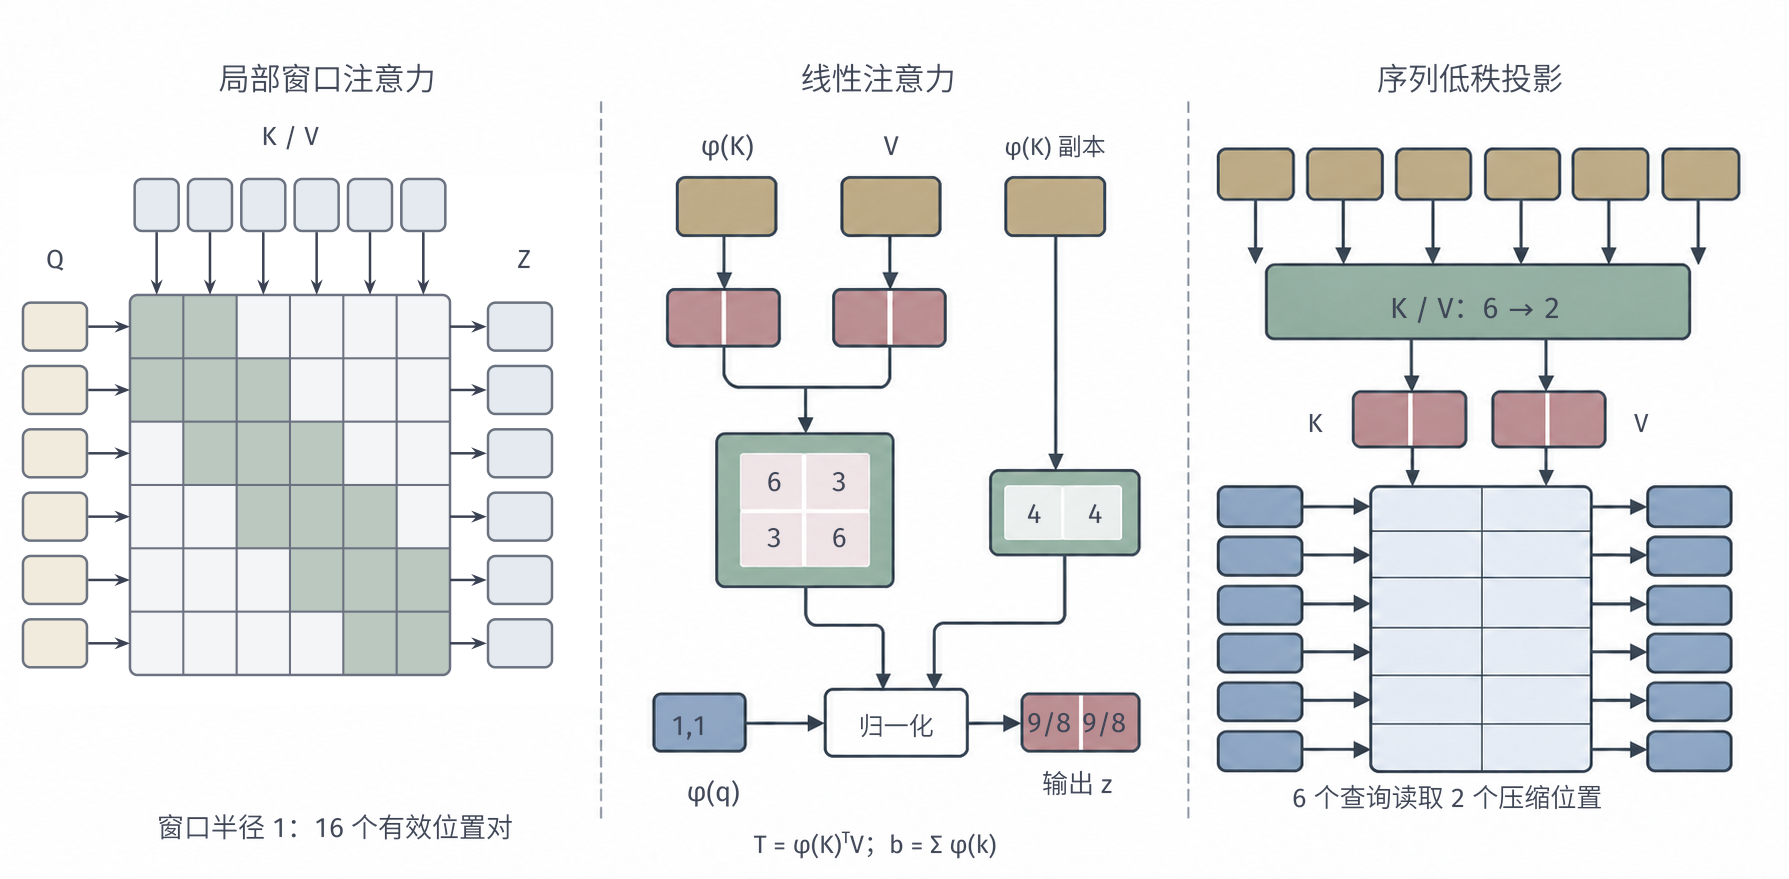
\includegraphics[width=151.469mm]{figures/05-neural-network-models/00-shared/generated/transformer-efficient-attention/figure.png}
  \caption{三条效率路线的具体读法，六个位置可按正文的“猫／在／院／里／追／狗”教学序列理解。左图中查询$\bm Q$对应各行，键值$\bm K/\bm V$对应各列，输出$\bm Z$逐行引出；着色格保留相邻位置的连接，白格表示删除的连接。中图给定教学键特征和值后，先累加外积和特征，再对查询归一化，数值由式\eqref{eq:transformer-linear-attention}复核。右图的示例投影把6个位置压成2个槽，右侧每行表示一个查询对两槽评分，颜色只表示存在连接。所有数值及压缩权重均为教学设定；三种方法并非对同一Softmax结果的等价改写。}
  \label{fig:transformer-efficient-attention}
\end{figure*}

图~\ref{fig:transformer-efficient-attention}把三条路线放回同一句“猫在院里追狗”，按字分成6个位置。左侧局部连接只保留当前位置及其左右邻居，把36个位置对减到16个；“追”这一行可以读取“里、追、狗”，却不能在本层直接读取“猫”。中间线性路线为键特征和值设置可手算的二维数值。

具体取$d_k=r=d_v=2$，依次给出六个位置的键特征和值：
\[
  \begin{array}{ccll}
    j&\text{词元}&\phi(\bm k_j)^{\top}&\bm v_j^{\top}\\
    1&\text{猫}&(1,\tfrac12)&(2,-1)\\
    2&\text{在}&(1,\tfrac12)&(2,-1)\\
    3&\text{院}&(\tfrac12,1)&(-1,2)\\
    4&\text{里}&(\tfrac12,1)&(-1,2)\\
    5&\text{追}&(\tfrac12,\tfrac12)&(3,3)\\
    6&\text{狗}&(\tfrac12,\tfrac12)&(3,3)
  \end{array}
\]
这些是教学设定的特征映射后键向量与投影后值向量，不是训练测量。例如，前面给出的特征映射将$\bm k_1=(0,-\log2)^{\top}$变为$(1,1/2)^{\top}$。要求非负的是成对相似度，值向量的坐标可以为负。

每一行分别贡献一个$2\times2$外积，按六个位置的顺序相加为
\[
  \begin{aligned}
    \bm T
      &=\begin{pmatrix}2&-1\\1&-1/2\end{pmatrix}
        +\begin{pmatrix}2&-1\\1&-1/2\end{pmatrix}\\
      &\quad+\begin{pmatrix}-1/2&1\\-1&2\end{pmatrix}
        +\begin{pmatrix}-1/2&1\\-1&2\end{pmatrix}\\
      &\quad+\begin{pmatrix}3/2&3/2\\3/2&3/2\end{pmatrix}
        +\begin{pmatrix}3/2&3/2\\3/2&3/2\end{pmatrix}\\
      &=\begin{pmatrix}6&3\\3&6\end{pmatrix}\text{。}
  \end{aligned}
\]
键特征也按同一位置顺序逐坐标累加：
\[
  \bm b=
  \begin{pmatrix}
    1+1+\tfrac12+\tfrac12+\tfrac12+\tfrac12\\
    \tfrac12+\tfrac12+1+1+\tfrac12+\tfrac12
  \end{pmatrix}
  =\begin{pmatrix}4\\4\end{pmatrix}\text{。}
\]
六项外积累加为$\bm T=\bigl[\begin{smallmatrix}6&3\\3&6\end{smallmatrix}\bigr]$，键特征相加为$\bm b=(4,4)^{\top}$；查询特征$(1,1)^{\top}$因而得到$(9/8,9/8)^{\top}$。具体地，$\bm T$的两行分别汇总两个键特征坐标对值的两个坐标的贡献；查询特征$(1,1)^{\top}$将两行相加，分子为$(9,9)$，分母为$(1,1)\bm b=8$，所以
\[
  \bm z_i^{\top}
    =\frac{(1,1)\bm T}{(1,1)\bm b}
    =\frac{(9,9)}8
    =(9/8,9/8)\text{。}
\]

也可以回到逐位置权重核对同一结果。该查询与前四个键的相似度均为$3/2$，与后两个键的相似度均为1，总和为8，因此权重依次为$3/16,3/16,3/16,3/16,1/8,1/8$。按这六个权重读取原值，得到
\[
  \begin{aligned}
    \bm z_i
      &=\frac3{16}\left[
          \begin{pmatrix}2\\-1\end{pmatrix}
         +\begin{pmatrix}2\\-1\end{pmatrix}
         +\begin{pmatrix}-1\\2\end{pmatrix}
         +\begin{pmatrix}-1\\2\end{pmatrix}\right]\\
      &\quad+\frac18\left[
          \begin{pmatrix}3\\3\end{pmatrix}
         +\begin{pmatrix}3\\3\end{pmatrix}\right]
       =\begin{pmatrix}9/8\\9/8\end{pmatrix}\text{。}
  \end{aligned}
\]
输出的两维对应值向量的两个特征坐标，不是两个位置的概率；本例两维恰好相等，来自这组六行教学数值的对称设置。逐位置计算相似度并按同一查询的总相似度归一化，再对值加权，与先汇总$\bm T,\bm b$再读取给出相同结果。这里各位置共同贡献一个固定大小的状态，查询再从状态读取。

右图则直接压缩位置：教学投影把前三个位置、后三个位置分别取平均，形成两个键值槽。所有6个查询仍各有一行，但每行只向两个槽评分。图中为便于核对令$\bm E_{\mathrm k}=\bm E_{\mathrm v}=\bm E$；Linformer的投影可以学习，也不必采用局部平均。这三幅图分别改变连接、核与可读取的表示，矩阵缩小分别来自删连接、改变核或合并位置，三个输出由各自的新计算定义。



\paragraph{优化中间存储与访存：FlashAttention}

前面三条路线改变了读取规则或公式，因而都是在“算什么”上做近似或取舍。还有一种浪费与此不同：即使要算的就是标准稠密注意力，把完整的$n\times n$得分、概率矩阵都写进显存、再读回来做加权，本身就耗费大量时间——GPU的算力往往不是瓶颈，数据在显存和计算单元之间来回搬运才是。\term{FlashAttention}保留标准稠密注意力的数学结果，通过分块计算和在线归一化，避免把完整得分、概率矩阵写入大容量显存。它在容量较小的片上存储中反复处理查询和键值块，减少完整中间矩阵的显存读写；反向传播按需要重算部分块，保存的统计量支持恢复这些局部计算\scite{dao2022flashattention}

理解在线Softmax可以只看一个查询。已处理的键集合上，维护最大得分$m$、归一化分母$s=\sum_j\exp(S_j-m)$和未归一化输出$\bm u=\sum_j\exp(S_j-m)\bm v_j$。新键块集合为$B$，块内最大值为$m_B$，更新为
\begin{equation}
  \begin{aligned}
    m'&=\max(m,m_B),\qquad c=\exp(m-m'),\\
    s'&=cs+\sum_{j\in B}\exp(S_j-m'),\\
    \bm u'&=c\bm u+\sum_{j\in B}\exp(S_j-m')\bm v_j\text{。}
  \end{aligned}
  \label{eq:transformer-online-softmax}
\end{equation}
旧统计乘以$c$，是在新最大值下重新表达同一批指数。遍历全部有效块后，输出为$\bm u/s$。初始为空时直接用第一个非空有效块建立统计，避免在全被掩码的块上做$-\infty-(-\infty)$。

沿用示例~\ref{ex:transformer-attention-numerical}，先处理得分$0,\log2$，得到$m=\log2$、$s=3/2$、$\bm u=(1/2,2)^{\top}$；再加入得分0和值$(1,1)^{\top}$，得到$s'=2$、$\bm u'=(1,5/2)^{\top}$，仍输出$(1/2,5/4)^{\top}$。分块没有把不同块分别归一化后简单求和，而是维护全局共同分母。

在固定头数和宽度下，FlashAttention把需要保存的注意力中间量从平方规模降到线性规模，实际训练还需保存其他模块激活。稠密位置对仍然存在，算术量仍为$O(n^2d)$；浮点运算顺序改变，结果可能有舍入差异。这里的“精确”指保留原稠密注意力公式，浮点舍入按实际执行顺序发生。速度收益依赖块大小、硬件和输入形状，其加速针对数据搬运与存储，位置对算术阶数保持原样。

图~\ref{fig:transformer-flashattention}对比“保存整个中间矩阵”与“算完一块就合并”。左侧常规路径显式形成完整得分与概率矩阵，右侧分块路径维护同一组$m,s,\bm u$，跨块更新使最终分母覆盖所有键；旧统计按新最大值重新缩放后，新旧键共同进入同一分母。对其他查询块重复这一过程，就能得到完整输出，而无需让完整得分、概率矩阵在大容量显存中落地。

\begin{figure*}[htbp]
  \centering
  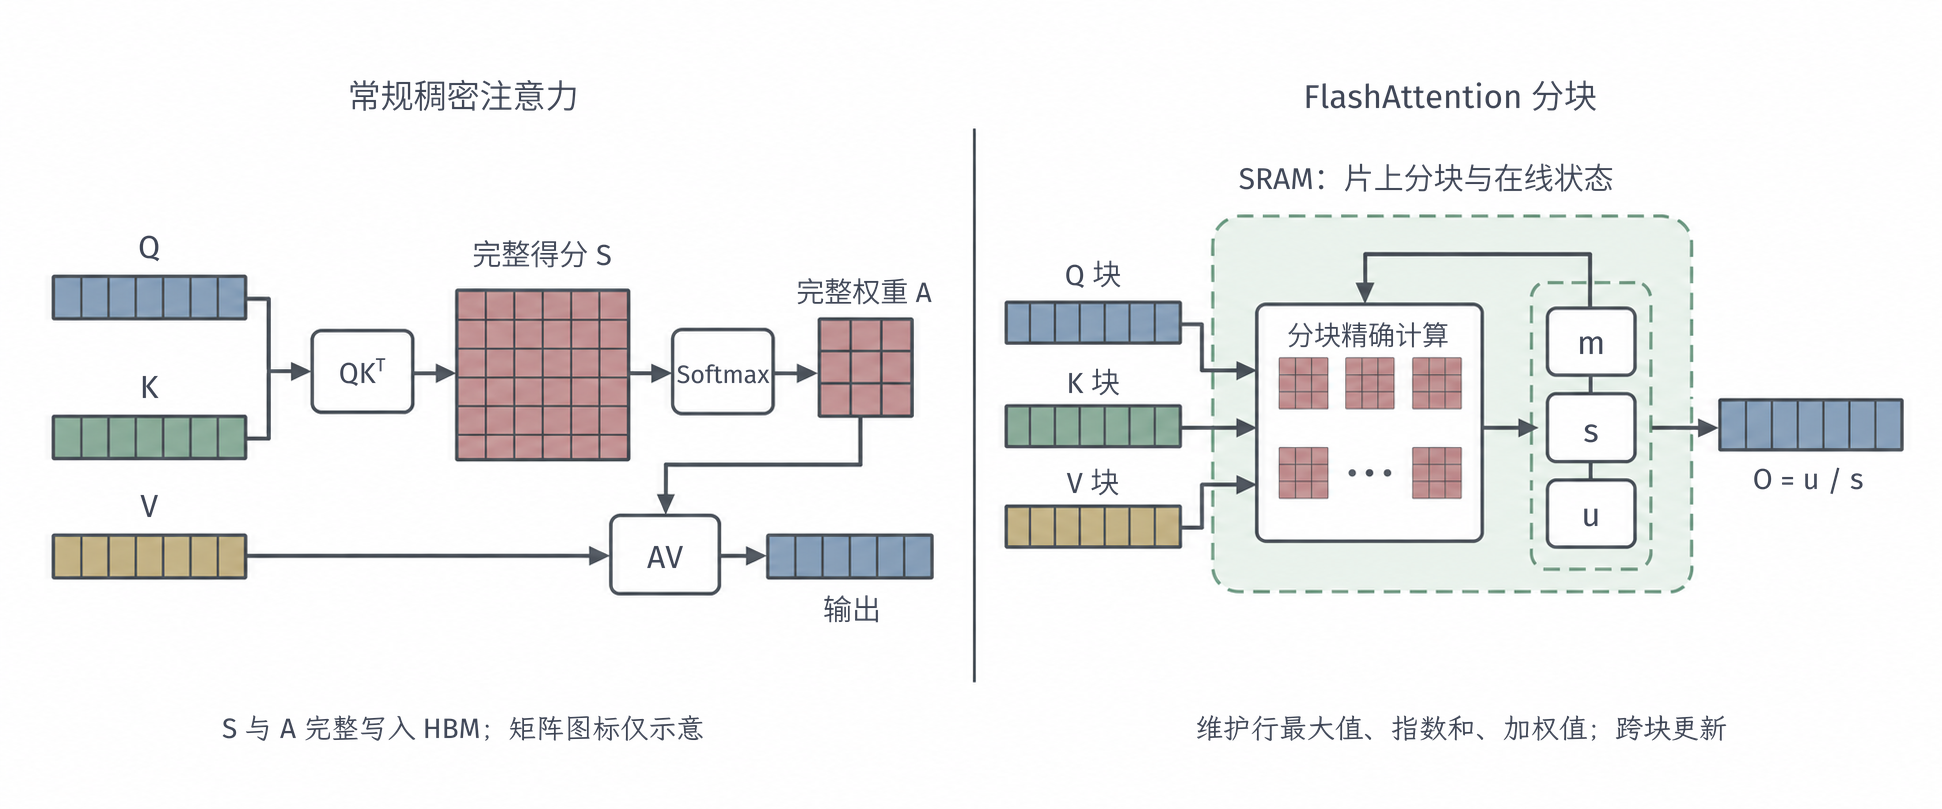
\includegraphics[width=164.423mm]{figures/05-neural-network-models/00-shared/generated/transformer-flashattention/figure.png}
  \caption{FlashAttention保留稠密注意力结果，改变中间结果的存储与合并方式。左图的常规实现把完整$\bm S,\bm A$写回容量较大的HBM；右图按块在HBM与容量较小的片上SRAM间搬运，只在片上保存当前块和在线统计$m,s,\bm u$。在线合并的分母覆盖全部键，输出与同一稠密注意力计算一致。图为存储与计算路径示意，教学数值在正文展开，反向重算细节省略。}
  \label{fig:transformer-flashattention}
\end{figure*}



\subsubsection{推理效率：历史缓存与请求分配}

增量生成需要反复读取历史键值，还要为不同长度请求分配存储。以下方法分别改变缓存内容与存储组织。

\paragraph{减少KV缓存容量与读取带宽：MQA与GQA}

解码时，标准MHA为每头保存一套键和值。在服务大模型时，这批KV缓存往往比模型本身还吃显存，因为模型参数只有一份、KV缓存却要按“并发请求数$\times$序列长度”成倍增长，而每个头的键值内容其实高度相似。一个自然的省法是让多个查询头共享同一组键和值：查询仍各自独立评分，但被查询的键值表不再每头存一份。\term{多查询注意力}（multi-query attention, MQA）保留多个查询头，让它们共享一组键值；\term{分组查询注意力}（grouped-query attention, GQA）将$h$个查询头分组，共享$g$组键值，其中$1\leq g\leq h$，是“每头一套”与“全体共享一套”之间的折中。设映射$\rho(a)$把查询头$a$分到键值组，则该头读取$\bm K_{\rho(a)},\bm V_{\rho(a)}$，仍有自己的一行Softmax和输出。

当$d_k=d_v$时，缓存元素数由$2Lnhd_k$变为$2Lngd_k$；MQA对应$g=1$，MHA对应$g=h$。例如$L=24$、$n=4096$、$h=16$、$d_k=64$、每元素2字节的单序列MHA缓存约为384 MiB，$g=4$的GQA约为96 MiB，MQA约为24 MiB。这组教学容量由键值元素数计算；权重、其他激活及分配管理另占存储。

\begin{figure*}[htbp]
  \centering
  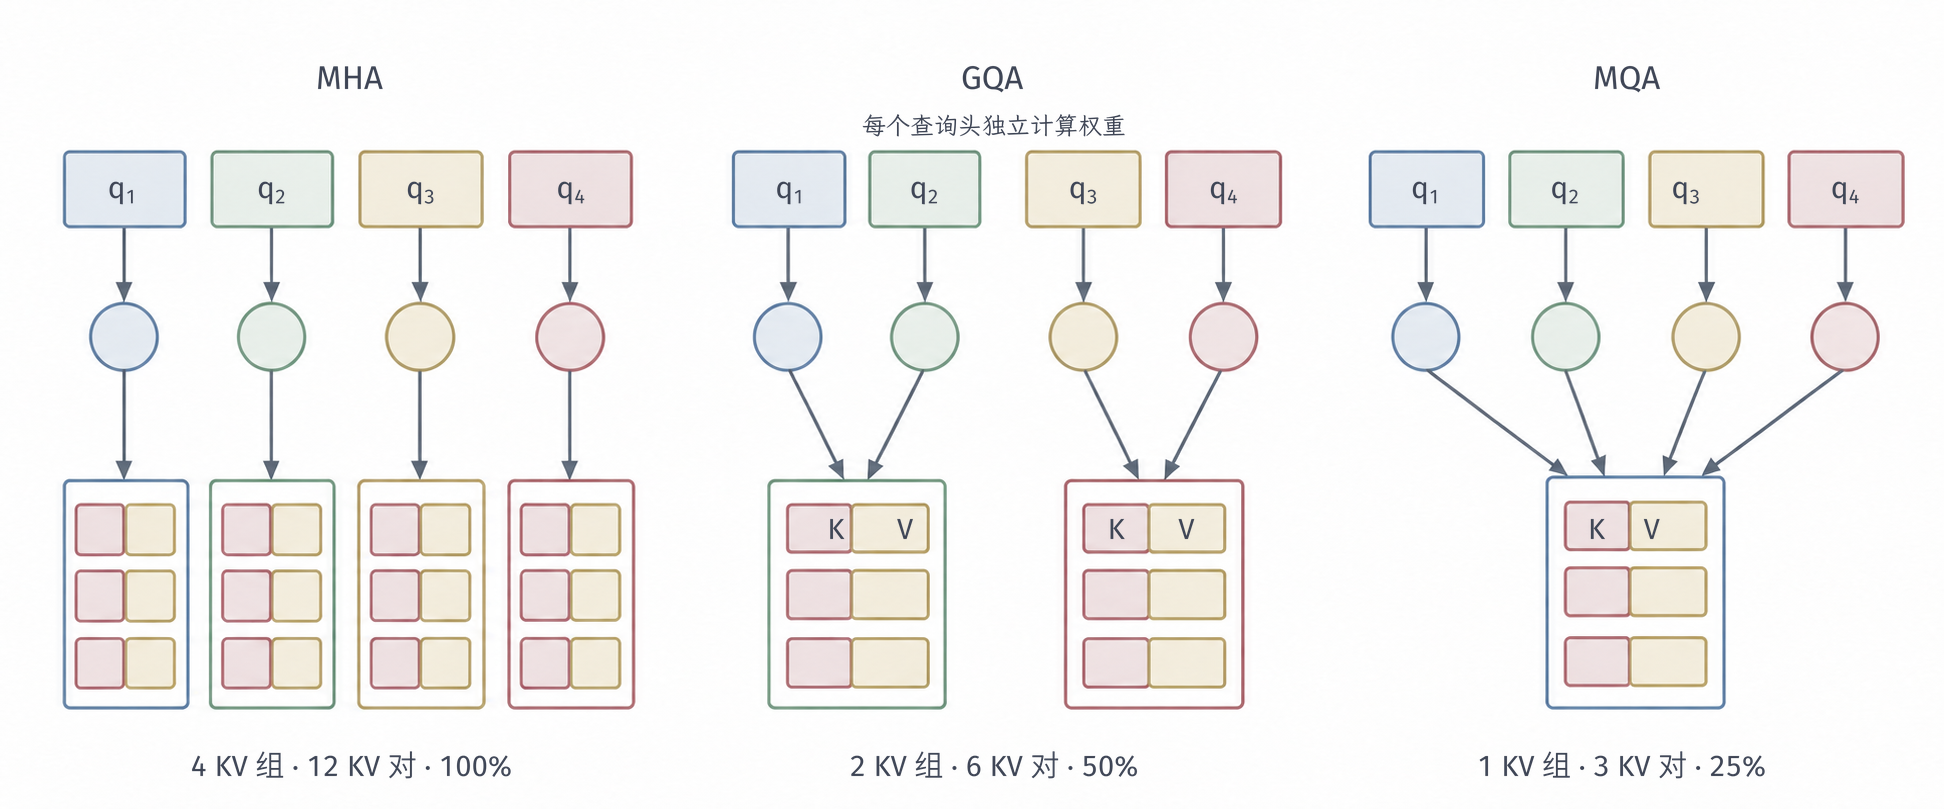
\includegraphics[width=164.592mm]{figures/05-neural-network-models/00-shared/generated/transformer-kv-sharing/figure.png}
  \caption{相同历史序列在MHA、GQA和MQA中的缓存布局。每个缓存小格代表一个历史位置在一组投影下的一对键和值；大框是一整组历史缓存，查询头的箭头指向所读取的缓存。4个查询头分别使用4组、2组或1组键值时，缓存为12、6或3对，下方标出的缓存容量相对于MHA依次为$100\%$、$50\%$和$25\%$。共享发生在键值表示及其存储上，各查询头仍独立计算注意力权重。图只计一层的一条序列，不含当前新位置追加的缓存。}
  \label{fig:transformer-kv-sharing}
\end{figure*}

图~\ref{fig:transformer-kv-sharing}固定3个历史位置“猫、追、狗”和4个新查询头，逐项数缓存中的键值对。MHA为每头保留3对，共12对；两组GQA保留6对；MQA只保留3对。MHA中同一历史位置对应4个缓存小格，表示该位置经过4组不同投影后产生的4对键值，四组投影分别产生自己的数值。共享后，不同查询仍分别与所读键匹配，所以可能得到不同的概率和输出。



Shazeer提出MQA以减少增量解码的键值访存，Ainslie等用GQA提供共享程度与质量之间的中间选择。共享减少了键值投影和缓存自由度，但查询头仍需分别匹配；查询仍逐头评分，评分算术量与缓存容量的$g/h$比例因此按不同操作统计。缓存读取若能在实现中复用，带宽需求才会相应改善，质量和速度都需要在给定模型与硬件上评价\scite{shazeer2019mqa} GQA还可由已有多头模型进行参数转换并继续训练，键值参数合并会改变表示，后续训练用于适应新的共享结构\scite{ainslie2023gqa}

\paragraph{提高KV缓存内存利用率：PagedAttention}

缓存容量之外，还存在分配问题，而且它是典型的“操作系统式”浪费而非容量问题：不同请求的长度持续增长，若像连续数组那样为每个请求预留一整段最大长度空间，请求较短时空闲区域无法分给别人，产生外部碎片；更常见的是，成百上千个请求往往共享同一段系统提示前缀，这份前缀的键值却被各自完整复制了许多遍。借鉴虚拟内存按页管理的思路，\term{分页注意力}（PagedAttention）把缓存划分为固定容量块，用块表把序列的逻辑位置映射到实际存储位置；序列增长时追加块，而不要求整段缓存连续。共同前缀可以引用同一批块，分叉后按需要复制，避免直接修改仍被其他请求读取的数据\scite{kwon2023pagedattention}

若每块容纳$b$个位置，长度$n$需要$\lceil n/b\rceil$块，最后一块的内部空余少于$b$个位置，另有块表和管理开销。原来连续存储中的外部碎片和重复前缀可由此减少，实际键值按所保存的位置继续占据空间，节省的是预留空闲、碎片和重复前缀。PagedAttention改变缓存寻址和共享，MQA/GQA改变键值组数，FlashAttention改变注意力中间结果的执行方式；三者处理不同问题，可在兼容实现中组合。块调度、并发服务和硬件算子的细节由系统卷展开。

图~\ref{fig:transformer-pagedattention}用两个请求演示块表的作用。为便于说明，把“请／解释／注意力／机制”和“请／解释／位置／编码”各视为4个词元，每块放2个位置。本图的词元位置与逻辑块均从0编号。A按物理块$3\rightarrow1$读取，B按$3\rightarrow4$读取，两者共享前缀块3，物理块2仍可供其他请求使用。读取A中位置$i=1$的“解释”时，逻辑块为$\lfloor1/2\rfloor=0$，块内偏移为1；查A块表索引0得到物理块3，再从其中的偏移1取出键和值。词元位置给出逻辑顺序，块表给出物理地址；物理块移动时保持块表对应，位置编码继续使用原逻辑编号。

\begin{figure*}[htbp]
  \centering
  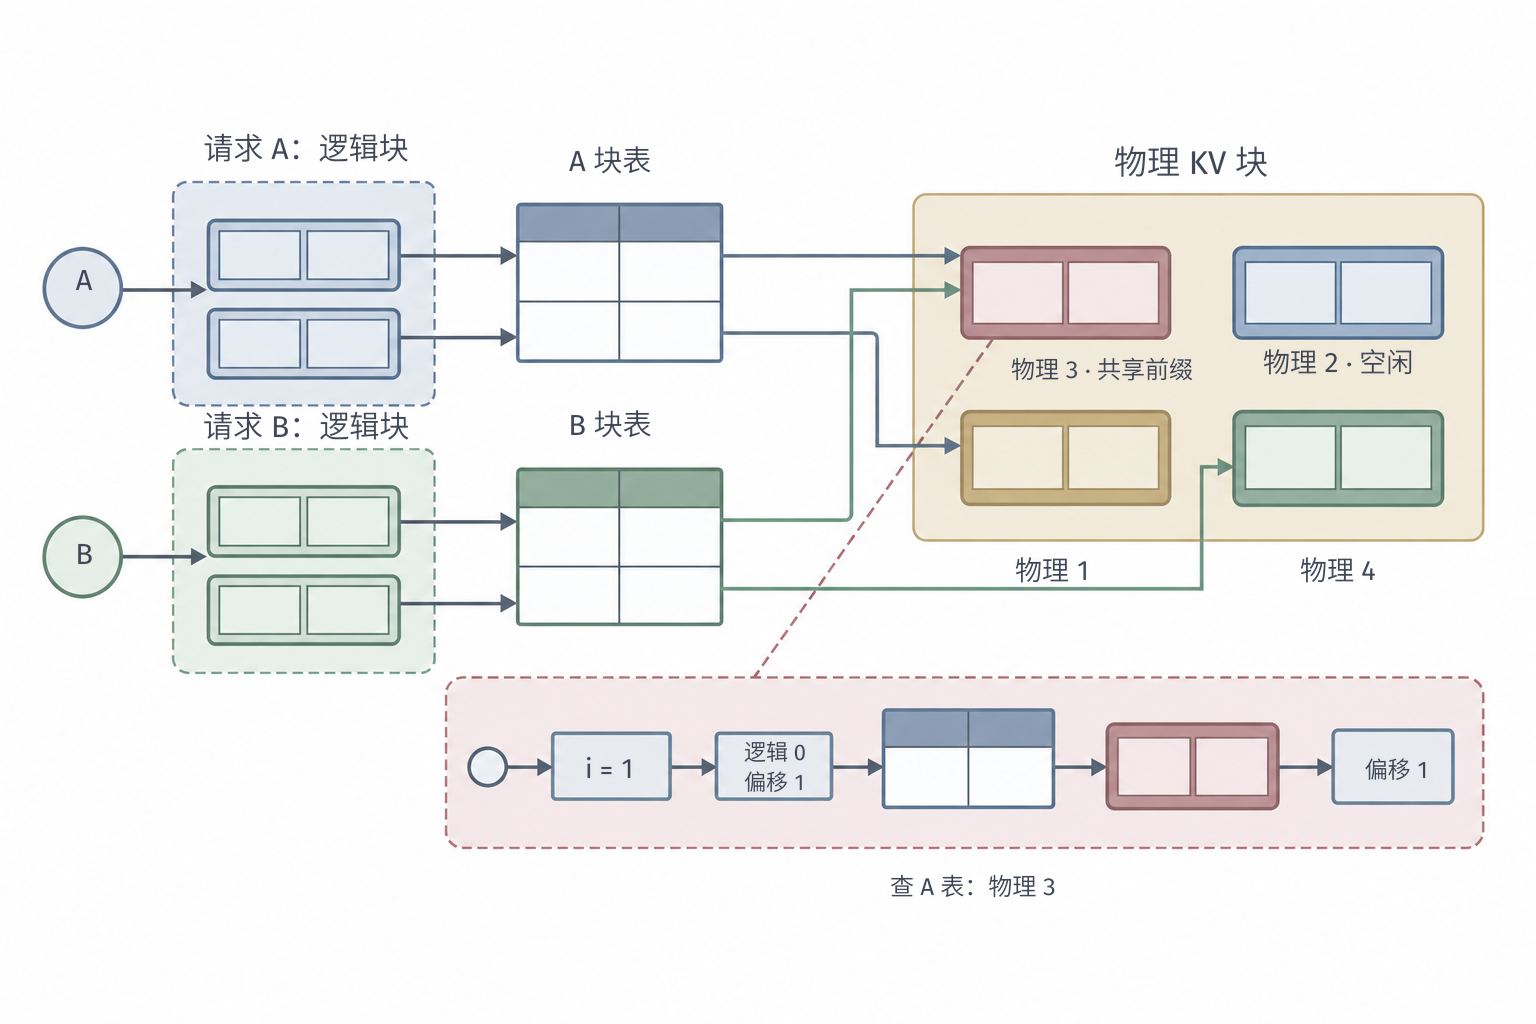
\includegraphics[width=130.048mm]{figures/05-neural-network-models/00-shared/generated/transformer-pagedattention/figure.png}
  \caption{分页键值缓存的具体寻址。上方两条请求按逻辑顺序分块，并用块表保存物理块编号；右侧为实际缓存布局。共享的物理块3只保存一份，A、B的后续各占一块，无需保持物理连续。底部展开一次“位置$\rightarrow$逻辑块$\rightarrow$物理块及偏移”的查找。词元位置、逻辑块和表索引从0开始；物理块编号用1至4标识。缓存小格表示对应的KV内容，正文中的词元例子用于解释寻址，并非把原始文本当作键值向量。}
  \label{fig:transformer-pagedattention}
\end{figure*}

\paragraph{不同扩展方向的比较}

表~\ref{tab:transformer-attention-extensions}把模型变化与实现变化分开。长序列算术量由实际位置连接与聚合决定，FlashAttention改善中间访存，分页改善键值分配。训练概率矩阵与解码历史缓存也有不同生命期，缩小其中一种只节省相应存储。门控、GQA、FlashAttention和分页可以在兼容实现中组合，因为它们分别作用于特征选择、键值组织、块内计算和缓存寻址。

\begin{table*}[htbp]
  \centering
  \small
  \begin{tabular}{@{}p{30mm}p{37mm}p{39mm}p{49mm}@{}}
    \toprule
    方法 & 主要改善对象 & 改变标准稠密读取？ & 代价或限制 \\
    \midrule
    前缀等掩码 & 可用信息与任务约束 & 改变允许连接 & 需防止目标或跨段泄漏 \\
    门控注意力 & 输入相关的特征选择 & 增加乘性调制 & 增加参数；不自动减少连接 \\
    稀疏注意力 & 位置对算术量 & 删除部分连接 & 范围受限；依赖连接模式 \\
    线性注意力 & 聚合算术量及历史状态 & 改变核或近似Softmax & 依赖特征维$r$与核表达能力 \\
    低秩注意力 & 交互维度与算术量 & 压缩键值位置 & 近似误差；因果性需另设计 \\
    FlashAttention & 中间存储与显存访存 & 保持公式，舍入可能不同 & 稠密算术仍为平方量级 \\
    MQA/GQA & KV容量与解码带宽 & 跨头共享键值参数 & 改变自由度；评分仍按查询头 \\
    PagedAttention & 缓存分配与前缀共享 & 保持逻辑读取规则 & 块表管理；真实键值仍占空间 \\
    \bottomrule
  \end{tabular}
  \caption{注意力扩展的主要目标与取舍。比较以相同有效输入、隐藏宽度与预测条件为前提；具体算术和存储量见各方法正文。降低算术量、减少访存、缩小KV缓存和减少内存碎片是不同指标，实际速度还取决于实现与硬件。}
  \label{tab:transformer-attention-extensions}
\end{table*}

\subsection{前馈层的扩展}
\label{sec:transformer-ffn-extensions}

同一位置的特征可以通过乘法分支调制，也可以交给少量被选中的前馈网络。门控改变特征变换形式，混合专家改变本次执行的网络分支；二者可以组合，跨位置读取仍由注意力等模块承担。

\subsubsection{门控前馈层：调制特征}

普通FFN先扩张特征，再用统一激活筛选。它有一个特点：某个中间特征是否通过、通过多少，完全由该特征自身的数值经固定激活函数决定，网络无法依据当前整行表示“主动地”决定放行还是关闭某类特征。在LSTM里我们已经见过更灵活的做法——用一个由输入算出的门去逐坐标控制信息通过。把这种乘法门控搬进前馈层，就能让“候选特征是什么”和“这批特征这次该放过多大比例”都成为输入相关的、可学习的决定：设置两条投影分支。\term{门控线性单元}（gated linear unit, GLU）用Sigmoid分支逐坐标调制另一分支；应用于Transformer前馈层的一般形式为
\begin{equation}
  \begin{aligned}
    \bm B&=\bm H\bm W_b+\bm1\bm b_b^{\top},\qquad
    \bm D=\bm H\bm W_g+\bm1\bm b_g^{\top},\\
    \operatorname{GFFN}(\bm H)&=(\bm B\odot\psi(\bm D))\bm W_o
                          +\bm1\bm b_o^{\top}\text{。}
  \end{aligned}
  \label{eq:transformer-gated-ffn}
\end{equation}
两条输入投影均从$d$到$d_g$，输出投影从$d_g$恢复$d$。GLU取$\psi=\sigma$，\term{GEGLU}取GELU，\term{SwiGLU}取SiLU，后两者分别由平滑激活产生乘性调制量。GELU或SiLU可以输出负值且不限定在$[0,1]$，这里的“门控”据乘法作用命名；LSTM的Sigmoid门另外受0至1的比例范围约束\scite{shazeer2020glu}

忽略偏置时，普通FFN约有$2dd_f$个参数，门控FFN约有$3dd_g$个参数。若保持这一参数预算，可取$d_g\approx2d_f/3$；比较同样中间宽度会同时改变参数和计算量。两投影分支提供新的特征组合，同时带来乘法尺度与参数配置的选择。泛化表现需结合相同预算下的任务与训练比较。

图~\ref{fig:transformer-gated-ffn}把“追”这一行的两条分支展开：候选特征$(2,-4)$与调制量$(0.5,2)$相乘，得到$(1,-8)$，再经输出投影恢复$d$维。第二维被放大，说明GEGLU、SwiGLU中的调制量不只是保留比例。这里用二维数值演示乘法，实际中间宽度由$d_g$决定；各位置仍独立处理，没有新增跨位置读取。

\begin{figure}[htbp]
  \centering
  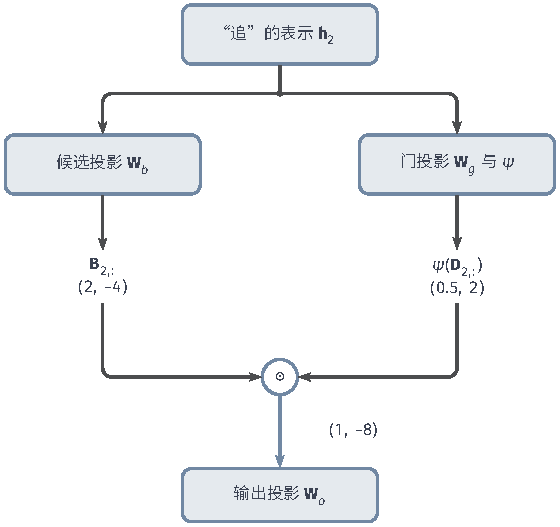
\includegraphics[width=94.791mm]{figures/05-neural-network-models/00-shared/tikz/transformer-gated-ffn/figure.pdf}
  \caption{门控前馈层对“追”的一次逐位置计算。候选特征$(2,-4)$与激活后的调制量$(0.5,2)$相乘为$(1,-8)$，再经输出投影恢复隐藏宽度。数值是教学假设；大于1的调制量适用于GEGLU或SwiGLU的解释，GLU的Sigmoid门则限制在0与1之间。猫、追、狗使用同一套参数分别计算，不发生跨位置读取。}
  \label{fig:transformer-gated-ffn}
\end{figure}

\FloatBarrier
\subsubsection{混合专家：前馈层的条件计算}
\label{sec:transformer-moe-extensions}

逐位置计算还可以按输入选择不同前馈网络。这里针对的是扩大模型时的一个矛盾：想让模型拥有更多可学习参数（更大的知识容量），可若每个位置都要把所有参数算一遍，计算量也随容量同步暴涨，划不来。\term{混合专家}（mixture of experts, MoE）的思路是把容量和单次计算量解耦：准备许多个专家网络，但每个位置只激活其中少数几个，于是总参数可以很多，单位置的实际计算却不随之增长。它设置多个专家和一个路由器，让不同位置使用不同专家组合。\term{专家}（expert）是可训练的特征变换网络，\term{路由器}（router）根据位置表示分配专家权重。设共有$e$个专家，单位置为$\bm h$，路由概率为$\bm p=\operatorname{softmax}(\bm W_{\mathrm r}^{\top}\bm h)$，$\bm W_{\mathrm r}\in\mathbb R^{d\times e}$。若只保留分数最大的$k$个专家集合$T_k(\bm h)$，可以计算
\begin{equation}
  \operatorname{MoE}(\bm h)
    =\sum_{a\in T_k(\bm h)}\widetilde p_a\,F_a(\bm h)\text{，}
  \label{eq:transformer-moe}
\end{equation}
其中$\widetilde p_a$可取选中概率重新归一化后的权重，也可按具体方法保留原概率；训练性质依赖这一约定。总专家参数随$e$增长，一次位置计算主要激活$k$个专家，加上路由器及共享模块的开销，模型存储计入全部专家，本次执行量按被选专家及公共部分分别统计\scite{shazeer2017}

路由可能把大量位置分给少数专家，造成容量不足或计算负载不均。容量限制决定多余位置如何处理，负载均衡辅助目标约束专家使用分布；它们会改变训练目标或输出过程。Top-$k$选择是离散的，常规反向传播只能在当前选择内对连续权重和专家求导，跨越选择边界的行为需要单独设计。若$k=1$并将唯一概率重新归一化为1，仅从这条乘权路径无法训练路由器，尤其需要保留可学习权重或其他训练信号。专家接到哪些输入、形成何种变换，由路由和监督共同学习。设备间派发与汇总还产生通信及调度成本，需在实际执行中另计。

图~\ref{fig:transformer-moe}把路由决策与专家计算分开。对“追”的同一个隐藏表示，假设路由概率为$(0.1,0.6,0.1,0.2)$。Top-2选择专家2和4，再除以所选概率之和$0.8$，得到权重$0.75$和$0.25$。两个专家都读取原隐藏表示$\bm h$，而不是读取路由概率；假设它们分别输出$(2,0)^{\top}$和$(0,4)^{\top}$，加权相加后才得到$(1.5,1)^{\top}$。专家1、3在本次没有执行，参数仍属于模型。这组概率与输出为手算构造，用来对应选择、执行和加权三个环节。

专家通常替换部分块中的FFN，注意力与残差仍可共享。不同位置可以选择不同专家，也可能选择相同专家；路由均衡控制位置怎样分派，输出比例继续由当前路由权重决定。

\begin{figure*}[htbp]
  \centering
  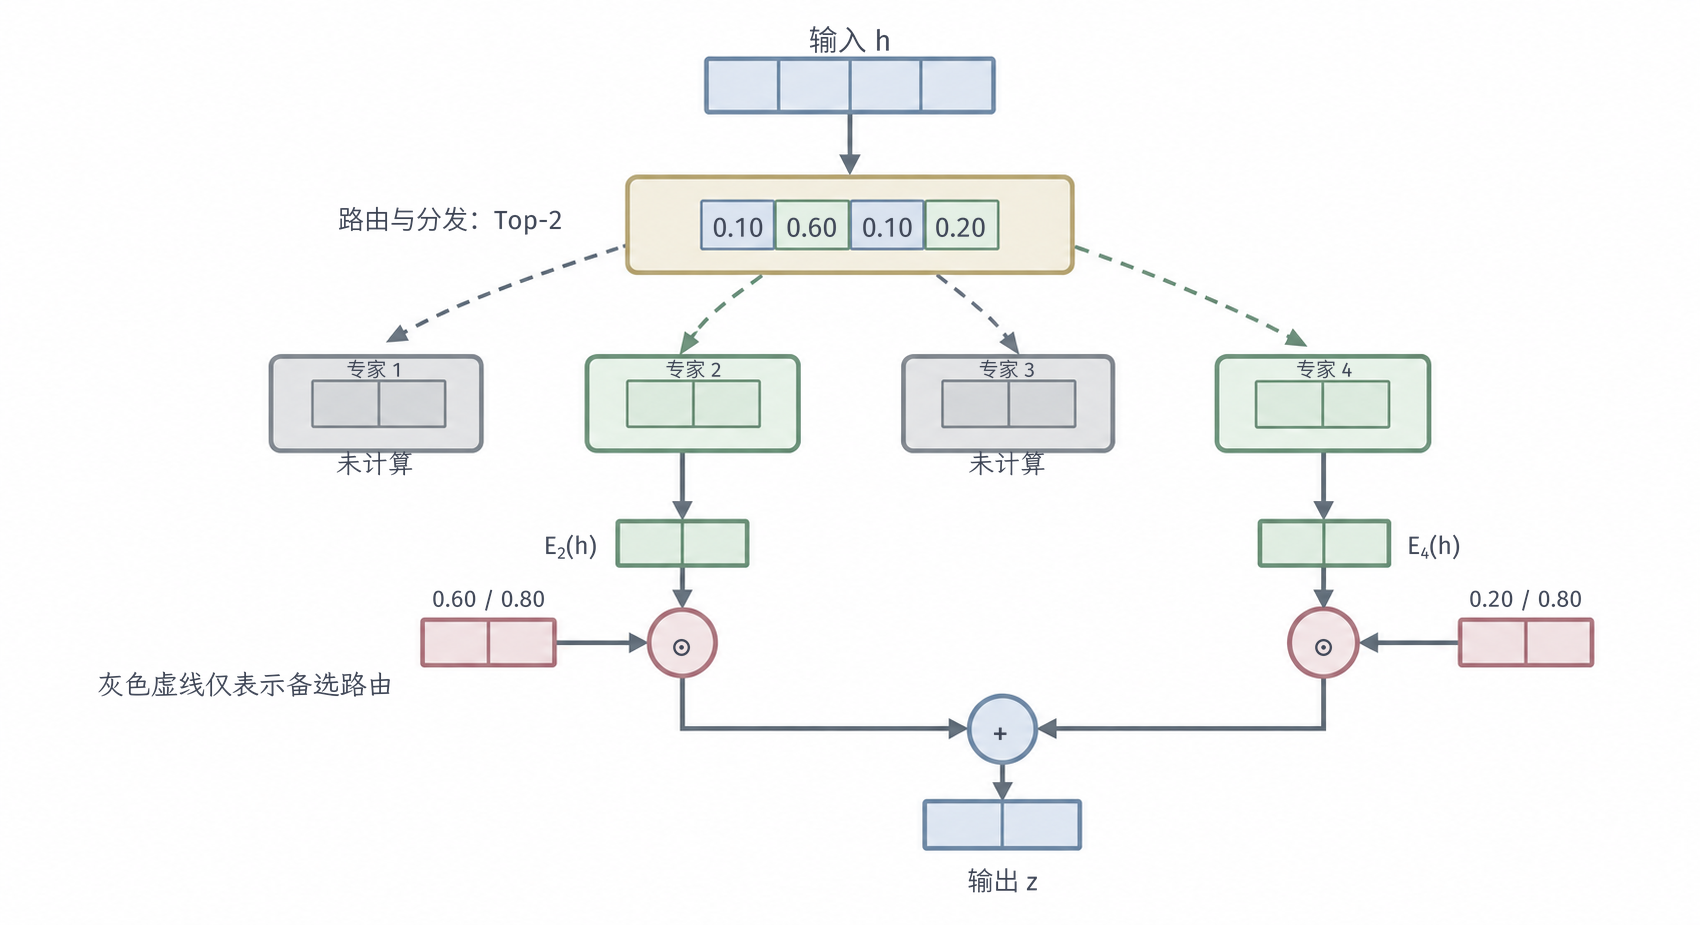
\includegraphics[width=143.933mm]{figures/05-neural-network-models/00-shared/generated/transformer-moe/figure.png}
  \caption{Top-2混合专家的一次完整计算，概率与二维专家输出均为教学设定。上方路由器选出专家2、4并给出重新归一化的权重；下方实线传递隐藏表示、专家结果及乘法所需的标量权重，路由器向各候选专家的虚线表示候选选择关系。专家输入始终是同一个$\bm h$，加权发生在专家输出之后，最终$0.75(2,0)^{\top}+0.25(0,4)^{\top}=(1.5,1)^{\top}$。灰色专家1、3本次不计算；图省略容量限制、辅助训练目标及块外残差。}
  \label{fig:transformer-moe}
\end{figure*}

\subsection{归一化的扩展}
\label{sec:transformer-normalization-extensions}

第\ref{sec:transformer-residual-normalization}节已经给出逐位置LayerNorm及其残差块形式。围绕归一化的种种变体，其实都在回答三个具体问题：沿哪些坐标求统计量、要不要减去均值、以及把归一化放在残差路径的哪一段。选择不同，被消去的信息就不同，信号与梯度通过深层网络的方式也不同。通用归一化公式、批归一化（BatchNorm）、实例归一化（InstanceNorm）和组归一化（GroupNorm）的完整说明见第\ref{sec:training-normalization}节，统计轴对照见表~\ref{tab:training-normalization-axes}。这里集中讨论Transformer中的因果限制、RMSNorm与残差位置。

\subsubsection{统计范围与因果限制}

对批量激活$\bm X\in\mathbb R^{b\times n\times d}$，三个轴分别是样本、位置和特征。式\eqref{eq:transformer-layernorm}固定样本和位置，只沿$d$个特征统计；不同位置不交换均值与方差，训练与预测均使用当前行的统计量，不需要运行均值。在这种逐位置用法中，每份统计都只由当前样本的一行特征形成。

完整已知的图像或离线编码可以使用跨空间、跨位置统计；因果解码则要求位置$i$的统计量不能包含$j>i$的激活。只要均值或方差读取了未来，即使注意力有三角掩码也会泄漏。若BatchNorm、InstanceNorm或GroupNorm采用跨整段统计，因果解码需要把统计范围限制到当时可用的激活，并使训练与预测采用对应方案。训练用全段统计、预测用前缀统计还会引入额外不一致；填充也不能作为有效观测参与统计。

\subsubsection{不减均值的RMSNorm}

中心化不是调整尺度的唯一方式。在极大模型中，LayerNorm里“求均值再逐坐标减去均值”这一步也要消耗可观的计算，而且对很多任务而言，真正需要控制的主要是向量整体幅度（决定点积大小），至于均值是否为零并不关键。\term{均方根归一化}（root mean square normalization, RMSNorm）因此做减法：不减去均值，只按坐标均方根缩放，省下中心化的开销：
\begin{equation}
  \operatorname{RMSNorm}(\bm x)
    =\bm\gamma\odot\frac{\bm x}
       {\sqrt{d^{-1}\sum_{k=1}^d x_k^2+\varepsilon}}\text{。}
  \label{eq:transformer-rmsnorm}
\end{equation}
这里采用常见的无平移形式。它与逐位置LayerNorm均只读取当前行，但少了均值计算和相减。给各坐标加同一常数时，LayerNorm的中心化结果不变，RMSNorm的结果一般会变；忽略$\varepsilon$时，二者都消去正比例整体缩放，实际耗时仍由实现与形状决定\scite{zhang2019rmsnorm}

逐位置统计只读当前行，同时可能消去行内均值或整体幅度。任务需要这些量时，应保留相应信息路径或调整统计方式。只调整整行长度的尺度归一化（ScaleNorm）见第\ref{sec:training-scalenorm}节；直接重参数化权重、而非统计激活的权重归一化（WeightNorm）见第\ref{sec:training-weightnorm}节。ScaleNorm调整激活长度，WeightNorm调整参数表示，与LayerNorm消除行均值的操作分别比较。

\subsubsection{归一化位置：Pre-LN、Post-LN与组合}

归一化的位置改变残差路径。Post-LN子层$\bm y=\operatorname{LN}(\bm x+F(\bm x))$的Jacobian矩阵为$\bm J_{\mathrm{LN}}(\bm I+\bm J_F)$，直接路径也要经过LN；Pre-LN的Jacobian矩阵为$\bm I+\bm J_F\bm J_{\mathrm{LN}}$，恒等路径绕过LN。Xiong等在特定初始化与模型分析下比较了两者的梯度尺度，并解释了原始Post-LN训练中学习率预热的重要性；论文的比较对应特定初始化与模型，其他深度和优化配置下的梯度及效果还需按实际计算检验\scite{xiong2020layernorm}

也可以在子层前和输出端分别归一化，控制输入与支路输出的尺度。例如，把子层的归一化输入记为$\bm u$，计算
\begin{equation}
  \begin{aligned}
    \bm u&=\operatorname{Norm}_{\mathrm{in}}(\bm x),\\
    \bm y&=\bm x+\operatorname{Norm}_{\mathrm{out}}(F(\bm u))\text{。}
  \end{aligned}
  \label{eq:transformer-combined-normalization}
\end{equation}
它与$\operatorname{Norm}(\bm x+F(\bm x))$不同，归一化这里只作用于新增支路，原输入直接进入相加。RMSNorm可放在前或后，LayerNorm也可采用不同位置；统计公式规定尺度怎样调整，放置位置规定哪条路径接受调整。归一化分母、可学习缩放、残差累积和末端读出共同影响信号，整网梯度需要沿这些模块的组合追踪，稳定条件同时涉及分母、缩放与分支累积。

\subsection{深层连接的扩展}
\label{sec:transformer-deep-connections}

直接堆叠残差块仍可能积累过大的更新或使深层分支难以学习。残差虽然给了恒等路径，但每个子层都无条件地把自己的增量全部加进去；层数很多时，这些增量叠加仍可能让表示尺度失控，而且在训练最初、各子层还很“生涩”时，让它们全力改变表示未必有利。一个自然的想法是给每个新增分支再配一个可调节的闸门，让网络自己决定这一层该往原表示里掺入多少新东西。一般子层可写为$\bm h^{(l)}=b_l\bm h^{(l-1)}+a_lF_l(\bm h^{(l-1)})$，其中$a_l$控制新增变换，$b_l$控制原表示的传递。固定缩放可以与深度相关，可学习缩放则让训练决定每条分支的影响；它们都要与归一化和初始化共同考虑。

\term{ReZero}给每条残差支路设置一个初始化为0的可学习标量$a_l$，使用$\bm h^{(l)}=\bm h^{(l-1)}+a_lF_l(\bm h^{(l-1)})$。在该残差堆叠不含其他破坏恒等路径的操作时，初始映射和局部Jacobian矩阵都是恒等。初始步骤中支路内部参数梯度受$a_l=0$抑制，但门参数有梯度$\partial\ell/\partial a_l=\langle\bm g^{(l)},F_l(\bm h^{(l-1)})\rangle$，门偏离0后支路开始收到监督。门参数首先决定支路参与的强度，内部参数可以从非零初始化开始\scite{bachlechner2020rezero}

门也可以是逐特征向量或输入相关函数，形成不同粒度的残差控制。向量门增加参数，自适应门增加计算和新的梯度路径；Sigmoid门如果希望初始接近关闭，偏置与饱和程度就需配合。更广的跨层连接还可把早期层的表示相加或拼接到深层，相加要求维度匹配，拼接会增加宽度并通常需要投影。这些改变影响表示复用、保存激活的数量和梯度路径，整网求导汇合所有分支，优化行为由实际复用和完整梯度共同决定。

图~\ref{fig:transformer-residual-extensions}对照归一化位置与支路缩放。把Norm移到子层之前，保留的是绕过Norm的恒等路径；在支路加入标量，控制的是新增变换的强度。这两个选择可以同时使用。

\begin{figure}[t]
  \centering
  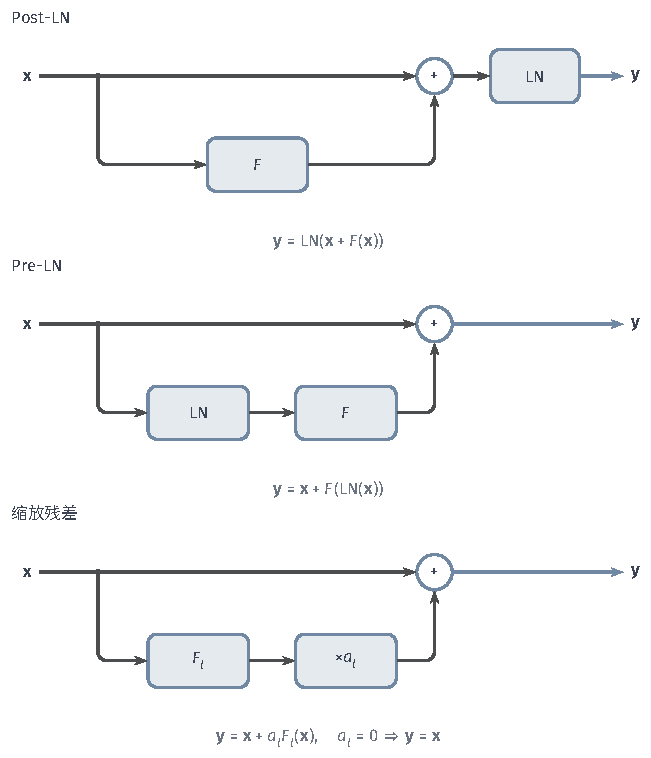
\includegraphics[width=110.225mm]{figures/05-neural-network-models/00-shared/tikz/transformer-residual-extensions/figure.pdf}
  \caption{把恒等路径放在同一水平线上比较三种残差组织。Post-LN的原输入在相加后仍通过LN；Pre-LN只有下方变换支路经过LN，恒等路径可以直接到达输出。第三行以$a_l$缩放新增变换，$a_l=0$时该子层输出等于输入；ReZero采用这一初值，图中省略可选归一化。各行上方路径传递原表示，下方路径计算新增变换，$+$为逐元素相加。}
  \label{fig:transformer-residual-extensions}
\end{figure}

\subsection{混合网络结构}
\label{sec:transformer-hybrid}

稠密注意力保存位置表示并显式读取它们，功能强大但代价是平方复杂度；卷积、循环、状态空间等模块则各有所长——它们擅长低成本地处理局部模式或用固定大小状态压缩历史，却不具备注意力那种“按内容任意直连”的能力。一个自然的工程问题是：能否让不同模块各管自己擅长的一段，而不是让注意力独自承担全部位置交互？局部窗口与固定容量历史状态可以由其他模块提供，与这份逐位置存储组合。若输入具有稳定局部模式，可以用卷积前端提取特征、降低分辨率，再把特征位置送入Transformer；窗口内部的卷积共享与注意力的内容相关读取承担不同职责。下采样减少序列长度，会明显改变后续平方位置对成本，也可能丢失细粒度信息，输出任务需要保留或恢复相应分辨率。

模块也可以交替堆叠。例如用状态空间模块压缩历史，用注意力层在保留位置之间进行显式检索；或者先用循环网络处理陆续到达的观测，再在给定窗口内交换信息。串联改变后一个模块接收到的表示，前端压缩决定后续可用内容，细节若没有保存在输出或旁路中，注意力就只读取剩下的表示。并行分支则可以分别形成局部与全局表示，再相加或拼接，维度、位置对齐和因果规则仍需一致。

各模块的成本沿实际执行累加：只要保留稠密注意力层，整段处理仍有平方量级的位置对计算；生成时，该层需保存随历史长度线性增长的KV缓存。训练中间存储另取决于实现，FlashAttention不必保存完整的平方规模注意力矩阵；固定状态节省相应模块的历史存储，保留的注意力层仍需自己的键值。前端、交替与并行是不同组织方式，应围绕任务需要的局部模式、精确历史读取、延迟和计算预算选择。

图~\ref{fig:transformer-hybrid}比较前端、交替与并行三种组织。它们分别改变输入粒度、层间分工与融合方式，使用哪一种都需要保持位置对应和信息可见规则。

\begin{figure*}[htbp]
  \centering
  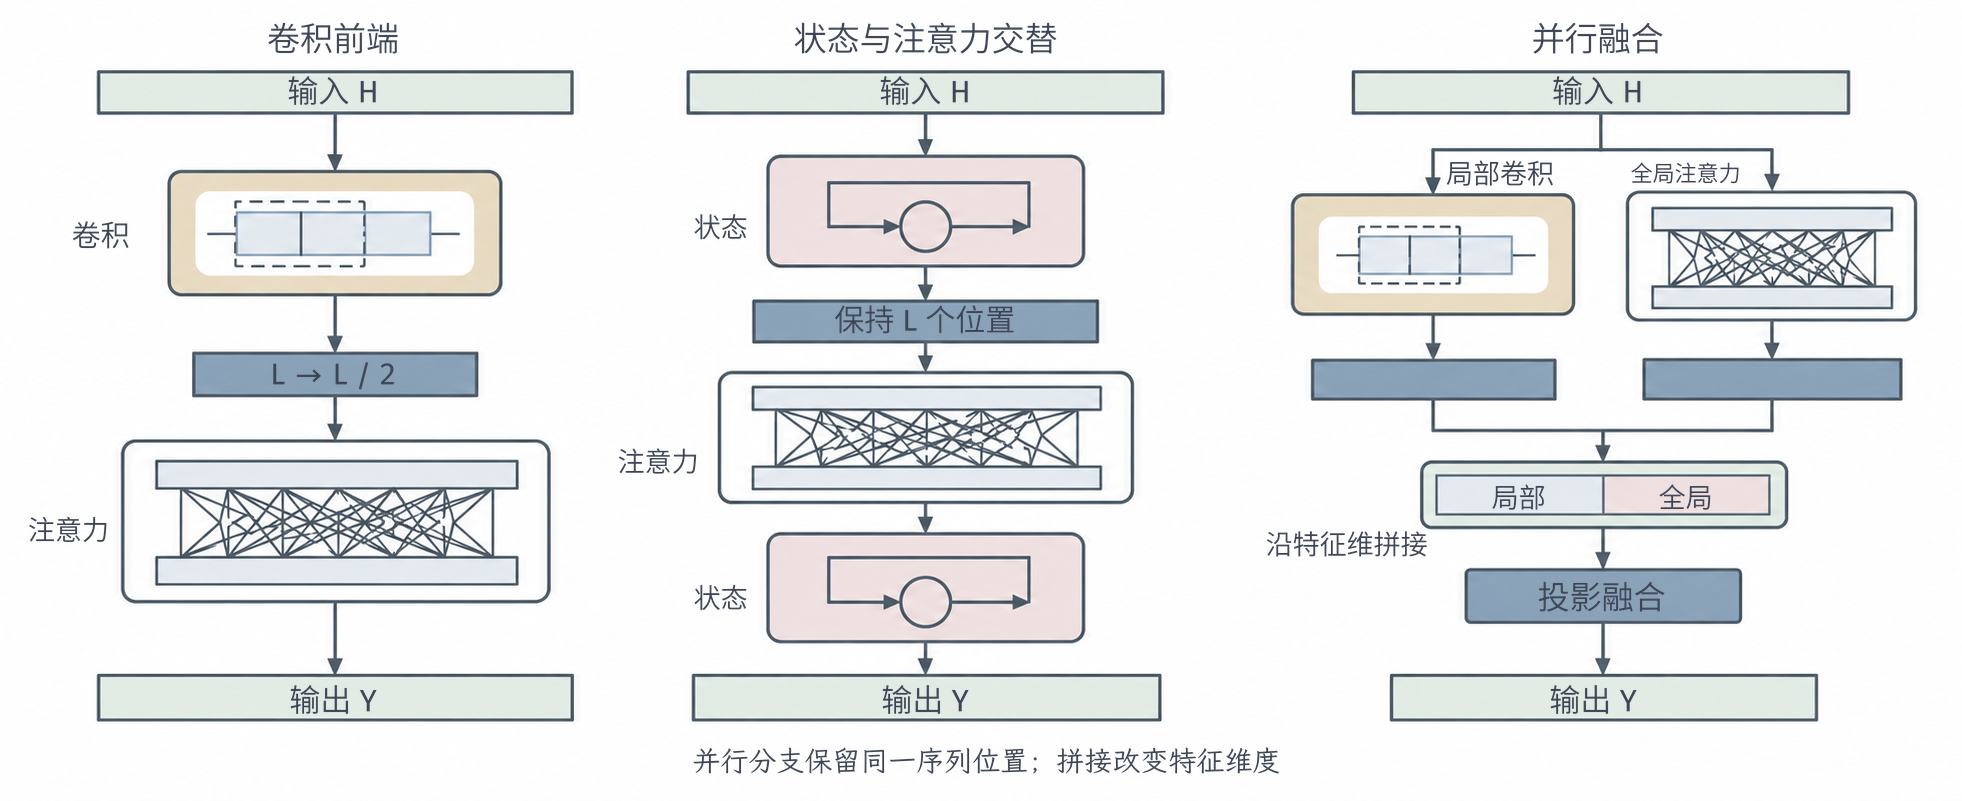
\includegraphics[width=166.116mm]{figures/05-neural-network-models/00-shared/generated/transformer-hybrid/figure.png}
  \caption{三种混合结构改变的是不同环节。左图在$L$为偶数、无填充的设置下，以窗口2、步长2的卷积前端将$L$个输入位置变成$L/2$个特征位置，再交给注意力；中图沿输入位置递推状态，并将各位置输出交给注意力层，随后继续交替；右图对同一序列并行计算局部卷积和注意力，拼接框沿特征维合并两路表示，再经投影融合。并行分支采用保持长度的位置对齐设置，所有分支还需满足任务的因果约束。}
  \label{fig:transformer-hybrid}
\end{figure*}

\FloatBarrier

\section{理论分析}
\label{sec:transformer-theory}

注意力能够跨位置读取，但读取范围、位置信息和数值尺度仍然限制所得表示。这里保留这些结构特有的条件；一般优化与统计推导沿用前面章节。

\subsection{表达能力}
\label{sec:transformer-expressivity}

没有位置或其他顺序线索、并采用对称汇聚的自注意力分类器，对相同词元的排列给出相同结果。因此$(a,b)$与$(b,a)$不能仅靠增加头数或层数得到区分。因果掩码则规定每个位置只能使用前缀，不能完成必须读取尚不可见后文的判断。

在固定长度、可学习位置编码及指定注意力与前馈结构下，Transformer可以逼近相应连续目标；Yun等的结论采用$L^p$积分误差，并允许深度随目标和精度改变\scite{yun2020transformeruniversal}。它不直接保证固定大小、不同掩码或归一化配置的模型具有同样能力，也不提供训练成功或长度外推保证。

\subsection{训练中的数值尺度}
\label{sec:transformer-convergence}

查询和键的尺度共同决定Softmax得分。权重过于集中时，评分路径的梯度可能变小；多头、残差和归一化又影响深层传播，因此需要结合投影尺度、归一化分母和梯度观察选择训练设置。一般光滑目标的优化结论见第\ref{sec:ffn-convergence}节，残差路径的存在本身不保证全局收敛。

硬Top-$k$路由还可能在专家集合切换时产生输出跳变。专家内部可微，不代表整个选择过程光滑；对这类结构，不能直接把连续网络的梯度结论当成路由参数的保证。固定的可见范围、正的归一化分母及实际采用的更新规则，都需要与训练条件对应。

\subsection{泛化性}
\label{sec:transformer-model-generalization}

在独立同分布序列和相应输入、参数及损失约束下，可以沿用复杂度或稳定性结论分析新样本风险，可参考\BookChapterRef{chap:deep-learning-theory}{卷3《基础、理论与可信性》的“深度学习的可学习性”章}。样本数应按实际独立记录计，同一文档的词元或重叠窗口不能各算一份独立证据。预训练、位置编码和缓存扩展了能够处理的输入，不自动保证新领域或更长序列上的误差；这些条件需要用对应数据单独检验。

\FloatBarrier

\section{常见应用}
\label{sec:transformer-applications}

应用中的完整模型需要把输入单位、可见信息、输出含义和监督位置对应起来。同一个Transformer骨架，之所以能用于看起来差异很大的任务，关键不在换了什么神秘结构，而在如何回答前面反复出现的那几个问题：输入切成什么单位、每个位置预测时允许看到谁、输出向量的每一维代表什么、损失加在哪一行。下面三个小节分别对应三种典型的对应方式——整段一个答案的分类、每个位置一个标签的标注，以及逐个产生输出的生成；阅读时可对照6.2节的输出头理解。以下沿用前文的网络块与损失，只展开从样本到预测的路径；数据构建、任务专用结构与评价方法由应用卷细化。

\subsection{文本分类与序列标注}
\label{sec:transformer-text-applications}

评论情感分类的样本是文本和类别。分词后查表形成嵌入，加位置表示，使用双向编码器得到上下文表示，再采用CLS或掩码池化读出，经Softmax分类。以“这部电影并不精彩”为例，编码器给“精彩”的表示可以读取否定上下文，整段分类头据此输出类别。否定关系提供这项任务需要的证据，模型通过哪些头和特征使用它，可以结合响应分析；最终预测由独立样本评价。

训练对评论计算交叉熵，嵌入、编码器和分类头共同更新；如果先使用已有模型，再训练任务头或微调部分层，需要明确哪些参数更新。推理使用同一分词与有效位置规则，输出整段概率。截断删去的文本可能包含判断证据，训练和测试的长度处理因而共同规定实际预测条件。

实体标注则将每个有效位置表示送入共享分类头，计算对应标签损失。若一个词被拆成多个子词，标签需选择监督首个子词、监督所有子词，或先聚合为词表示，推理时也用同一规则。逐位置Softmax分别形成标签概率，跨位置标签组合若有约束，还需由相应输出模型联合处理。离线标注读取整段，流式标注使用因果或有限延迟范围，这个约束比“采用编码器还是解码器”的名称更直接。

\subsection{序列转换与生成}
\label{sec:transformer-generation-applications}

机器翻译训练使用源句$x$和包含EOS的目标$y$。源嵌入和编码器产生$\bm H_{\mathrm s}$，目标输入右移，因果自注意力读取真实目标前缀，交叉注意力读取有效源位置，以式\eqref{eq:transformer-conditional-loss}更新两侧嵌入、所有网络块和词表输出层。源词和目标词通过条件似然共同训练，注意力权重由这份翻译监督学习软对应。

推理时源端只编码一次，各目标层还可预先缓存该层交叉注意力的源键值。目标从BOS开始，每次前向为当前输入计算并追加各层自注意力键值，再由词表头产生下一词元分布。选出的词元作为下一次输入，逐步延长缓存，遇到EOS或长度上限停止。不同层的投影参数不同，因此源交叉键值与目标自注意力键值都按层保存。束搜索存在多个候选前缀时，可以共享未变的缓存内容，分叉后的修改则需各自维护或按写入时复制处理。

文本续写不需要独立源编码器。已给定提示先做预填充，末位置输出预测提示后的第一个词元；把选出的词元作为新输入，在各层追加缓存，得到下一词元分布。续写读取已经产生的完整前缀，训练则读取真实前缀；两种输入来源决定模型实际经历的上下文。选择温度、采样或搜索策略会影响输出，评价需使用实际采用的生成过程。

\subsection{图像分类}
\label{sec:transformer-vision-applications}

图像具有二维网格位置，注意力读取的却是“一串向量”，要把图像交给Transformer，先要解决“怎样把二维图像变成一串位置”。一个朴素想法是把每个像素当一个位置，但像素数量动辄上百万，平方注意力完全无法承受；而且单个像素几乎不含语义，模型真正需要交互的是“一小块一小块”的局部区域。因此折中的做法是把图像切成若干小块，每块经一次投影变成一个向量，块与块之间再做注意力——位置数从像素数降到块数，变得可负担。\term{视觉Transformer}（Vision Transformer, ViT）将图像分成块，分别嵌入后进行位置间注意力，再读出图像类别\scite{dosovitskiy2020vit}

设图像高宽为$H,W$、通道数为$c$，块边长为$p$，并暂设$H,W$可被$p$整除，则块数为$n=HW/p^2$，每块展平向量$\bm x_i\in\mathbb R^{p^2c}$。投影后的输入为
\begin{equation}
  \bm h_i^{(0)}=\bm W_{\mathrm p}^{\top}\bm x_i+\bm b_{\mathrm p}+\bm p_i,
  \qquad \bm W_{\mathrm p}\in\mathbb R^{p^2c\times d}\text{。}
  \label{eq:transformer-vit-input}
\end{equation}
位置索引按固定网格顺序排列，位置表示须保留块与空间位置的对应。加入专用分类位置后，共有$n+1$行表示，经编码器、末端归一化和分类头产生概率，以图像标签交叉熵训练。图~\ref{fig:transformer-vit}把图像块、序列表示与分类输出连接起来。

\begin{figure*}[htbp]
  \centering
  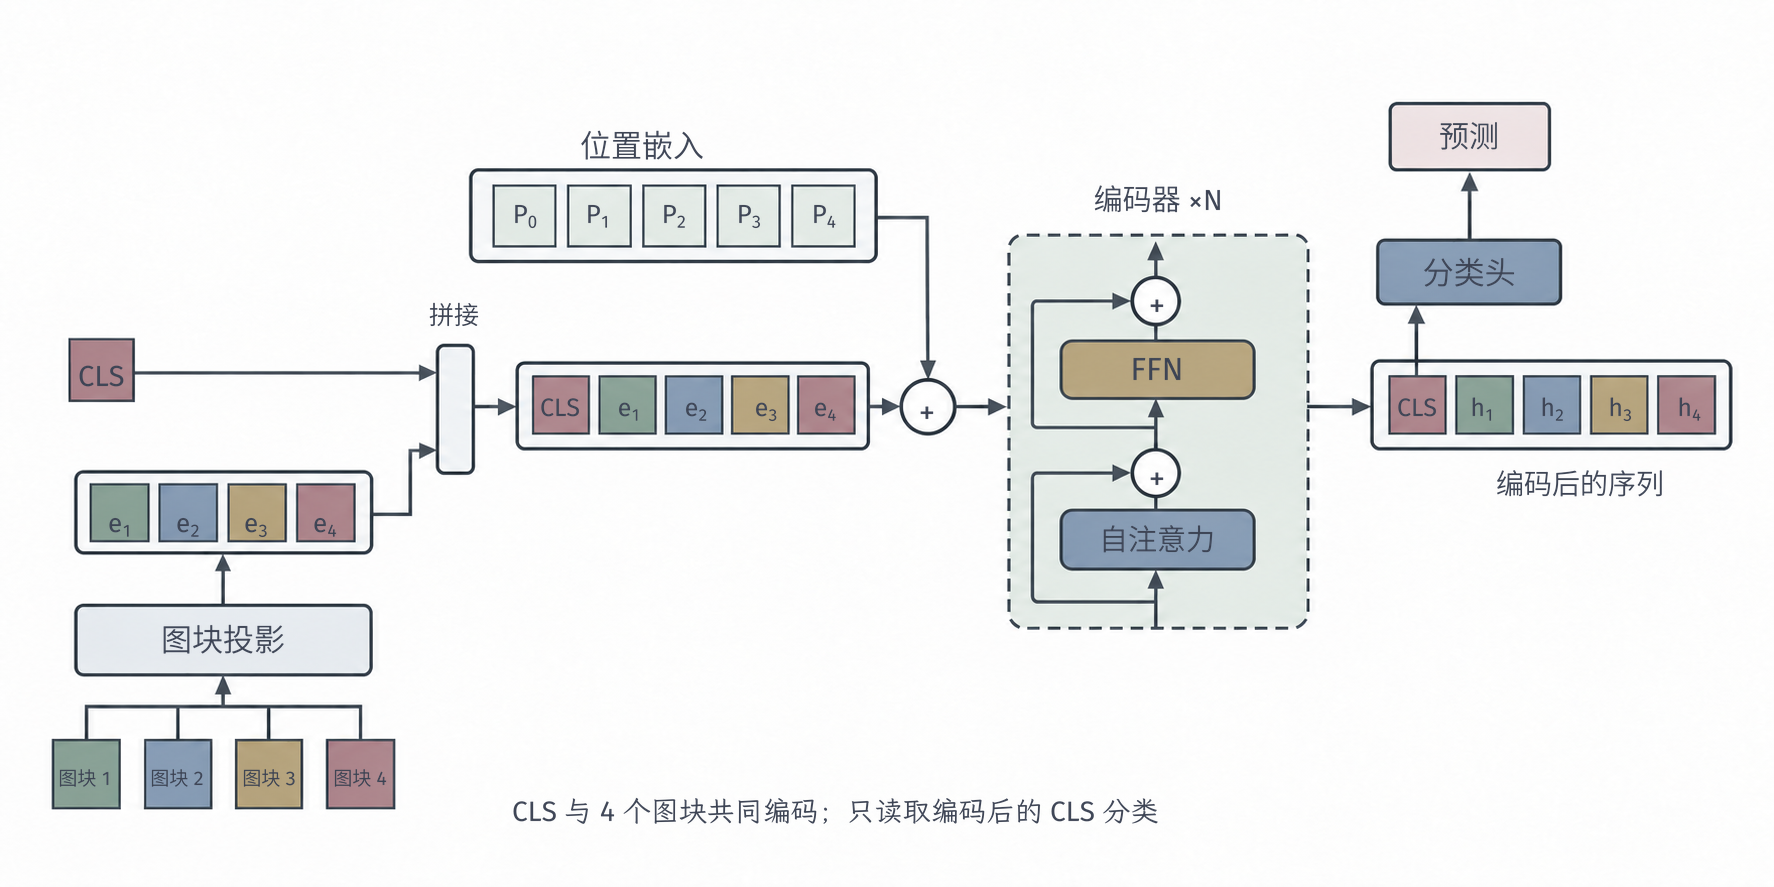
\includegraphics[width=150.199mm]{figures/05-neural-network-models/00-shared/generated/transformer-vit/figure.png}
  \caption{ViT将图像组织为序列的过程。四个示意图像块按固定空间顺序编号；每块展平后通过同一线性投影形成$\bm e_i$。在开头加入可学习CLS表示，为五行分别加入位置向量，再送入双向编码器。分类头只读取末层CLS行，其他图像块通过注意力参与其形成。图像块色块仅为结构示意，不声明实际像素尺寸，也不是识别实验样本。}
  \label{fig:transformer-vit}
\end{figure*}

图像块之间可直接交互，但块内部结构在原始ViT中经一次线性投影进入表示，没有逐层卷积的局部共享假设。较小的$p$保留更细的位置划分，同时使$n$增长；固定图像尺寸时，稠密注意力位置对数与$p^{-4}$同阶，前馈层的块数成本则与$p^{-2}$同阶。改变图像分辨率会改变网格和位置数量，可学习位置表常需按空间网格插值；插值提供新网格的位置向量，分类质量还取决于新增图像细节与已学规则的匹配。数据量、预训练、局部模块和增强会影响实际效果，ViT与卷积模型的实际比较需要固定数据、训练投入和评价目标，局部归纳假设与预训练知识共同影响结果。

\FloatBarrier
\section{本章小结}
\label{sec:transformer-summary}

Transformer把序列中的位置依赖转为显式读取：内容表示给出查询、键和值，位置表示和掩码约束怎样匹配以及哪些位置可见，多头注意力形成不同聚合，逐位置前馈网络再组合这些特征。残差和归一化让这套计算能够层层堆叠。与循环注意力相比，它可以同时更新已知位置。逐步生成时，新的输出依次成为后续条件，缓存保存已完成的位置计算以便复用。

结构与资源的选择需要同时看任务。双向读取适合完整输入理解，因果读取满足在线与生成条件，交叉注意力将源目标表示分开。位置扩展提供不同距离规律，门控和专家改变特征选择；稀疏、线性和低秩路线改变读取结构或公式，FlashAttention保留稠密计算而减少中间访存，MQA/GQA缩小键值组数，PagedAttention改善缓存分配与共享。减少哪一种开销、改变哪一种表示自由度，决定了这些方法的组合与取舍。

损失沿值读取、评分、特征变换及直接残差路径汇集为参数梯度，训练进展与预测风险再据各自条件评价。得分尺度、归一化分母、残差深度和长度共同影响学习，独立样本数、参数约束、数据分布和评价目标共同约束风险结论。由此可以回答章首的问题：直接位置交互使已知输入的计算更易并行，但可靠预测还取决于可见范围是否正确、任务信息是否保留，以及学习结果是否在实际使用条件下得到检验。

\paragraph{扩展阅读}
原始Transformer、BERT与GPT-3论文见第\ref{sec:transformer-common-architectures}节，可结合本章公式核对输入、掩码、归一化与监督位置。
